\chapter{Evaluation}

\section{Customer Requirements}

\subsection{General Objective Evaluation}

\subsubsection{-Data can added to the database easily}
\textbf{Was the Objective Fulfilled?} \newline
This objective has been fulfilled successfully. The data fields have been labeled so that the user knows what data they need to enter into the field. Evidence for this can be in figure \ref{fig:}. The information in which the user must enter has been grouped together in a group box, for the convenience of the user, which is evidenced in figure \ref{fig:} .

 The system clearly shows when the user has entered valid or non valid data by creating a green border around each data field. Evidence for the current validation for my system can be found in figure \ref{fig:}. 

Adding a Product Employee and a Member are all done in a similar fashion which reduces the time having to learn how to add each aspect to the system. The system will clearly state whether the product, member or employee has been added successfully or not.\newline

\textbf{Evidence} \newline


\subsubsection{-Data can be edited within the system easily.}
\textbf{Was the Objective Fulfilled?} \newline
This objective has been fulfilled. The user has to enter the ID of the item they would like to edit, and the edit interface will allow them to change the data. As specified above, the data inputs have been grouped together which is convenient for the user, the edit interface also has a clear edit button in the bottom right hand corner of the interface in which the user can click when they have finished editing the information. The button is bright green which means it is obvious for the user to see.\newline

\textbf{Evidence} \newline

\subsubsection{-Easy to understand the layout of the information.}
\textbf{Was the Objective Fulfilled?} \newline
This objective was fulfilled but improvements could be made. Information was placed in group boxes where possible to organise the information displayed to the user \newline

\textbf{Evidence} \newline




\subsubsection{-Easy to locate a product within the system.}
\textbf{Was the Objective Fulfilled?} \newline
This objective was fulfilled. To locate a product within the system, the user can use the search window. There are multiple ways to access the search window, which decreases the difficulty of accessing it. The structure of the search window is easy to understand and the user can search for data by entering keywords into the search field and the system will return the search results instantly. The results of the search can be re-ordered by clicking on the column headings. This is evidenced on page \pageref{}. The keywords can match any data that is display in the product table, be it the ProductID, ProductName, Price Category.\newline

\textbf{Evidence} \newline





\subsubsection{-The system as a whole, should be clear and easy to use.}
\textbf{Was the Objective Fulfilled?} \newline

\textbf{Evidence} \newline





\subsection{Specific Objective Evaluation}


\subsubsection{-For an image to be displayed when an item is searched for (identifying a product if the Product information is unknown}
\textbf{Was the Objective Fulfilled?} \newline
This objective was not fulfilled. I did not fulfill this objective as i had problems during the implementation stage when displaying the ProductImages in a table. Each time the contents of the Product Table changed, the system would stop responding for about 10-15 seconds before displaying the images and the contents of the search result. Therefore, in order to make the flow of control of the system more fluid, i decided to remove this functionality from the system. \newline

\textbf{Evidence} \newline





\subsubsection{-For the Stock control system to be integrated with the process of selling items. This is so that the stock is automatically updated when a product is sold.}
\label{-For the Stock control system to be integrated with the process of selling items. This is so that the stock is automatically updated when a product is sold.}
\textbf{Was the Objective Fulfilled?} \newline
This objective was fulfilled. When a customer purchases an item(s), when the invoice is saved to the system, the system automatically deducts the quantity of each product the customer purchased, from the current stock of the product.\newline

\textbf{Evidence} \newline




\subsubsection{-For the new process of selling products to be quicker, to minimize the time for people queuing.}
\textbf{Was the Objective Fulfilled?} \newline
This objective was not fulfilled. This objective was not fulfilled because currently, my client uses a bar code scanner that automatically finds the product in the system and adds it to the order when the bar code is scanned. This objective has been poorly worded as my system could not be any faster than the current system of selling products. However, if you combine the time spent creating the order and time spent changing all the stock of the products, my system completes this process much faster than my clients current system, as currently my client has to change the stock of the products each day to match the sales made that day. This process is done automatically in my system which is evidenced on page \pageref{}.\newline

\textbf{Evidence} \newline




\subsubsection{-For the current stock to automatically update when the products are bought}
\textbf{Was the Objective Fulfilled?} \newline
This objective is the exactly the same as "-For the Stock control system to be integrated with the process of selling items. This is so that the stock is automatically updated when a product is sold". This objective has already been fulfilled.




\subsubsection{-For a reminder message to pop up when stock needs to be moved from storage to the front of the vets. }
\textbf{Was the Objective Fulfilled?} \newline
This objective has been fulfilled. When a user logs into the system, the system will check if any products need to be moved between locations or if any products need to be restocked. If there are less than 5 of a specific product in the Shop then the user will be told that stock needs to be moved form the storage room to the shop and if the total stock of the product is less than 5 then the user will be told that that product needs to be restocked.\newline

\textbf{Evidence} \newline




\subsubsection{-For each and every product to be categorised for easy identification is the Product Name and ID is unknown.}

\textbf{Was the Objective Fulfilled?} \newline
This objective has been fulfilled. whent he user adds aproduct to the system they must choose from two drop down menus (QComboBox) in order to categorise the product. The first they choose the aniamal it is for, i.e horse, dog, cat and whether the product comes under food or health care. When the user wants to search for all products under, for example, Dog Health Care, they can simply go to the search window and enter 'Dog Health Care' into the search field and the system will return all the products under that category.

\textbf{Evidence} \newline





\subsubsection{-To calculate how much stock will be required for next month.}
\label{stock-eval}
\textbf{Was the Objective Fulfilled?} \newline
This objective has been fulfilled. The system records the daily and weekly sales of each product. These sales are then plotted to a graph on the stock management interface, which is used to predict the sales for the up coming week. Predicting the sales from the daily sales usually produces are more accurate prediction.

\textbf{Evidence} \newline





\subsubsection{-For the MemberID to be entered and the identity of the client is confirmed to make sure they are a member.}
\textbf{Was the Objective Fulfilled?} \newline
This objective was fulfilled. When the user wants to edit a member in the system they must enter the MemberID of each member. If the member is in the system their information will be displayed to the user, if not, then the user is told that the Member is not currently in the system. This process is done automatically when the user enters a MemberID into the creating order interface, it will either apply a 10 percent discount if the Member is stored in the system and will not apply it if they are not in the system.

\textbf{Evidence} \newline




\subsubsection{-For Keyboard Shortcuts to be availble for the system to be accessed faster.}
\textbf{Was the Objective Fulfilled?} \newline
this objective has been fulfilled. A large variety of keyboard shortcuts have been produced for the system to make the flow of control much faster. The keyboard shortcuts use relevant keys, relating to there function. For example to \textbf{A}dd a product tot he system, the user can press CTRL and \textbf{A}. 

\textbf{Evidence} \newline




\subsubsection{-To Format a well structured receipt that is easy for the customer to read and to understand}
\textbf{Was the Objective Fulfilled?} \newline
This objective has been fulfilled. The invoice for an order has been created using HTML. The top left hand corner of the invoice displays the company logo and location and contact information. The invoice also displays the customer the invoice is due to along with all the products in the order along with their price. The invoice also creates a date and time the invoice was created and sent. The products are displayed in a table to make them easy to read for the customer.

\textbf{Evidence} \newline




\subsubsection{-Allowing the Order of the products in the database to be changed.(i.e. Max - Min Price, A-Z ect \ldots)}
\textbf{Was the Objective Fulfilled?} \newline
This objective has been fulfilled. On every table within my system. The user has the ability to click on a column heading and the contents of the table will be sorted by that column. For example, by default all the products will be sorted by their ProductID's. If the user clicks on the price column heading the products will be sorted by price, lowest to highest. If the user then clicks on the price column header again, it will sort the products by price highest to lowest.

\textbf{Evidence} \newline


\subsection{Core Objective Evaluation}

\subsubsection{-For the Stock control system to be integrated with the process of selling items. This is so that the stock is automatically updated when a product is sold.}
\textbf{Was the Objective Fulfilled?} \newline
This objective is also found under the general objectives section. this can be found on page \pageref{-For the Stock control system to be integrated with the process of selling items. This is so that the stock is automatically updated when a product is sold.} . It was concluded that this objective had been fulfilled.
\textbf{Evidence} \newline



\subsubsection{-For the Stock to automatically update itself.}
\textbf{Was the Objective Fulfilled?} \newline

\textbf{Evidence} \newline




\subsubsection{-To calculate how much stock will be required for next month.}
\textbf{Was the Objective Fulfilled?} \newline
This objective has previously been evaluated in the General Objective Evaluation, which can be found on page \pageref{stock-eval}. It was concluded that this objective has been fulfilled
\textbf{Evidence} \newline



\subsection{Other Objective Evaluation}


\subsubsection{-allowing the Order of the products in the database to be changed.(i.e. Max - Min Price, A-Z etc \ldots)}
\textbf{Was the Objective Fulfilled?} \newline

\textbf{Evidence} \newline



\subsubsection{-For Keyboard Shortcuts to be available for the system to be accessed faster.}
\textbf{Was the Objective Fulfilled?} \newline

\textbf{Evidence} \newline



\subsubsection{-To Format a well structured receipt that is easy for the customer to read and to understand}
\textbf{Was the Objective Fulfilled?} \newline

\textbf{Evidence} \newline












\section{Effectiveness}

\subsection{Effectiveness of General Objectives}





















\subsubsection{-Data can added to the database easily}
\textbf{Evaluation Criteria:} \newline
\begin{itemize}
\item{}
\item{}
\item{}
\end{itemize}

\textbf{Judgment and Evidence:} \newline





\subsubsection{-Data can be edited within the system easily.}
\textbf{Evaluation Criteria:} \newline
\begin{itemize}
\item{}
\item{}
\item{}
\end{itemize}

\textbf{Judgment and Evidence:} \newline





\subsubsection{-Easy to understand the layout of the information.}
\textbf{Evaluation Criteria:} \newline
\begin{itemize}
\item{}
\item{}
\item{}
\end{itemize}

\textbf{Judgment and Evidence:} \newline





\subsubsection{-Easy to locate a product within the system.}
\textbf{Evaluation Criteria:} \newline
\begin{itemize}
\item{}
\item{}
\item{}
\end{itemize}

\textbf{Judgment and Evidence:} \newline







\subsubsection{-The system as a whole, should be clear and easy to use.}
\textbf{Evaluation Criteria:} \newline
\begin{itemize}
\item{}
\item{}
\item{}
\end{itemize}

\textbf{Judgment and Evidence:} \newline









\subsection{Effectiveness of Specific Objectives}













\subsubsection{-For an image to be displayed when an item is searched for (identifying a product if the Product information is unknown}
\textbf{Evaluation Criteria:} \newline
\begin{itemize}
\item{}
\item{}
\item{}
\end{itemize}


\textbf{Judgment and Evidence:} \newline








\subsubsection{-For the Stock control system to be integrated with the process of selling items. This is so that the stock is automatically updated when a product is sold.}
\textbf{Evaluation Criteria:} \newline
\begin{itemize}
\item{}
\item{}
\item{}
\end{itemize}


\textbf{Judgment and Evidence:} \newline






\subsubsection{-For the new process of selling products to be quicker, to minimize the time for people queuing.}
\textbf{Evaluation Criteria:} \newline
\begin{itemize}
\item{}
\item{}
\item{}
\end{itemize}

\textbf{Judgment and Evidence:} \newline







\subsubsection{-For the current stock to automatically update when the products are bought}
\textbf{Evaluation Criteria:} \newline
\begin{itemize}
\item{}
\item{}
\item{}
\end{itemize}

\textbf{Judgment and Evidence:} \newline






\subsubsection{-For a reminder message to pop up when stock needs to be moved from storage to the front of the vets. }
\textbf{Evaluation Criteria:} \newline
\begin{itemize}
\item{}
\item{}
\item{}
\end{itemize}

\textbf{Judgment and Evidence:} \newline








\subsubsection{-For each and every product to be categorised for easy identification is the Product Name and ID is unknown.}
\textbf{Evaluation Criteria:} \newline
\begin{itemize}
\item{}
\item{}
\item{}
\end{itemize}

\textbf{Judgment and Evidence:} \newline









\subsubsection{-To calculate how much stock will be required for next month.}
\textbf{Evaluation Criteria:} \newline
\begin{itemize}
\item{}
\item{}
\item{}
\end{itemize}

\textbf{Judgment and Evidence:} \newline









\subsubsection{-For the MemberID to be entered and the identity of the client is confirmed to make sure they are a member.}
\textbf{Evaluation Criteria:} \newline
\begin{itemize}
\item{}
\item{}
\item{}
\end{itemize}

\textbf{Judgment and Evidence:} \newline








\subsubsection{-For Keyboard Shortcuts to be available for the system to be accessed faster.}
\textbf{Evaluation Criteria:} \newline
\begin{itemize}
\item{}
\item{}
\item{}
\end{itemize}

\textbf{Judgment and Evidence:} \newline








\subsubsection{-To Format a well structured receipt that is easy for the customer to read and to understand}
\textbf{Evaluation Criteria:} \newline
\begin{itemize}
\item{}
\item{}
\item{}
\end{itemize}

\textbf{Judgment and Evidence:} \newline







\subsubsection{-Allowing the Order of the products in the database to be changed.(i.e. Max - Min Price, A-Z ect \ldots)}\textbf{Evaluation Criteria:} \newline
\begin{itemize}
\item{}
\item{}
\item{}
\end{itemize}

\textbf{Judgment and Evidence:} \newline









\section{Learnability}

\section{Usability}

\section{Maintainability}

\section{Suggestions for Improvement}

\section{End User Evidence}

\pagebreak
\subsection{Questionnaires}

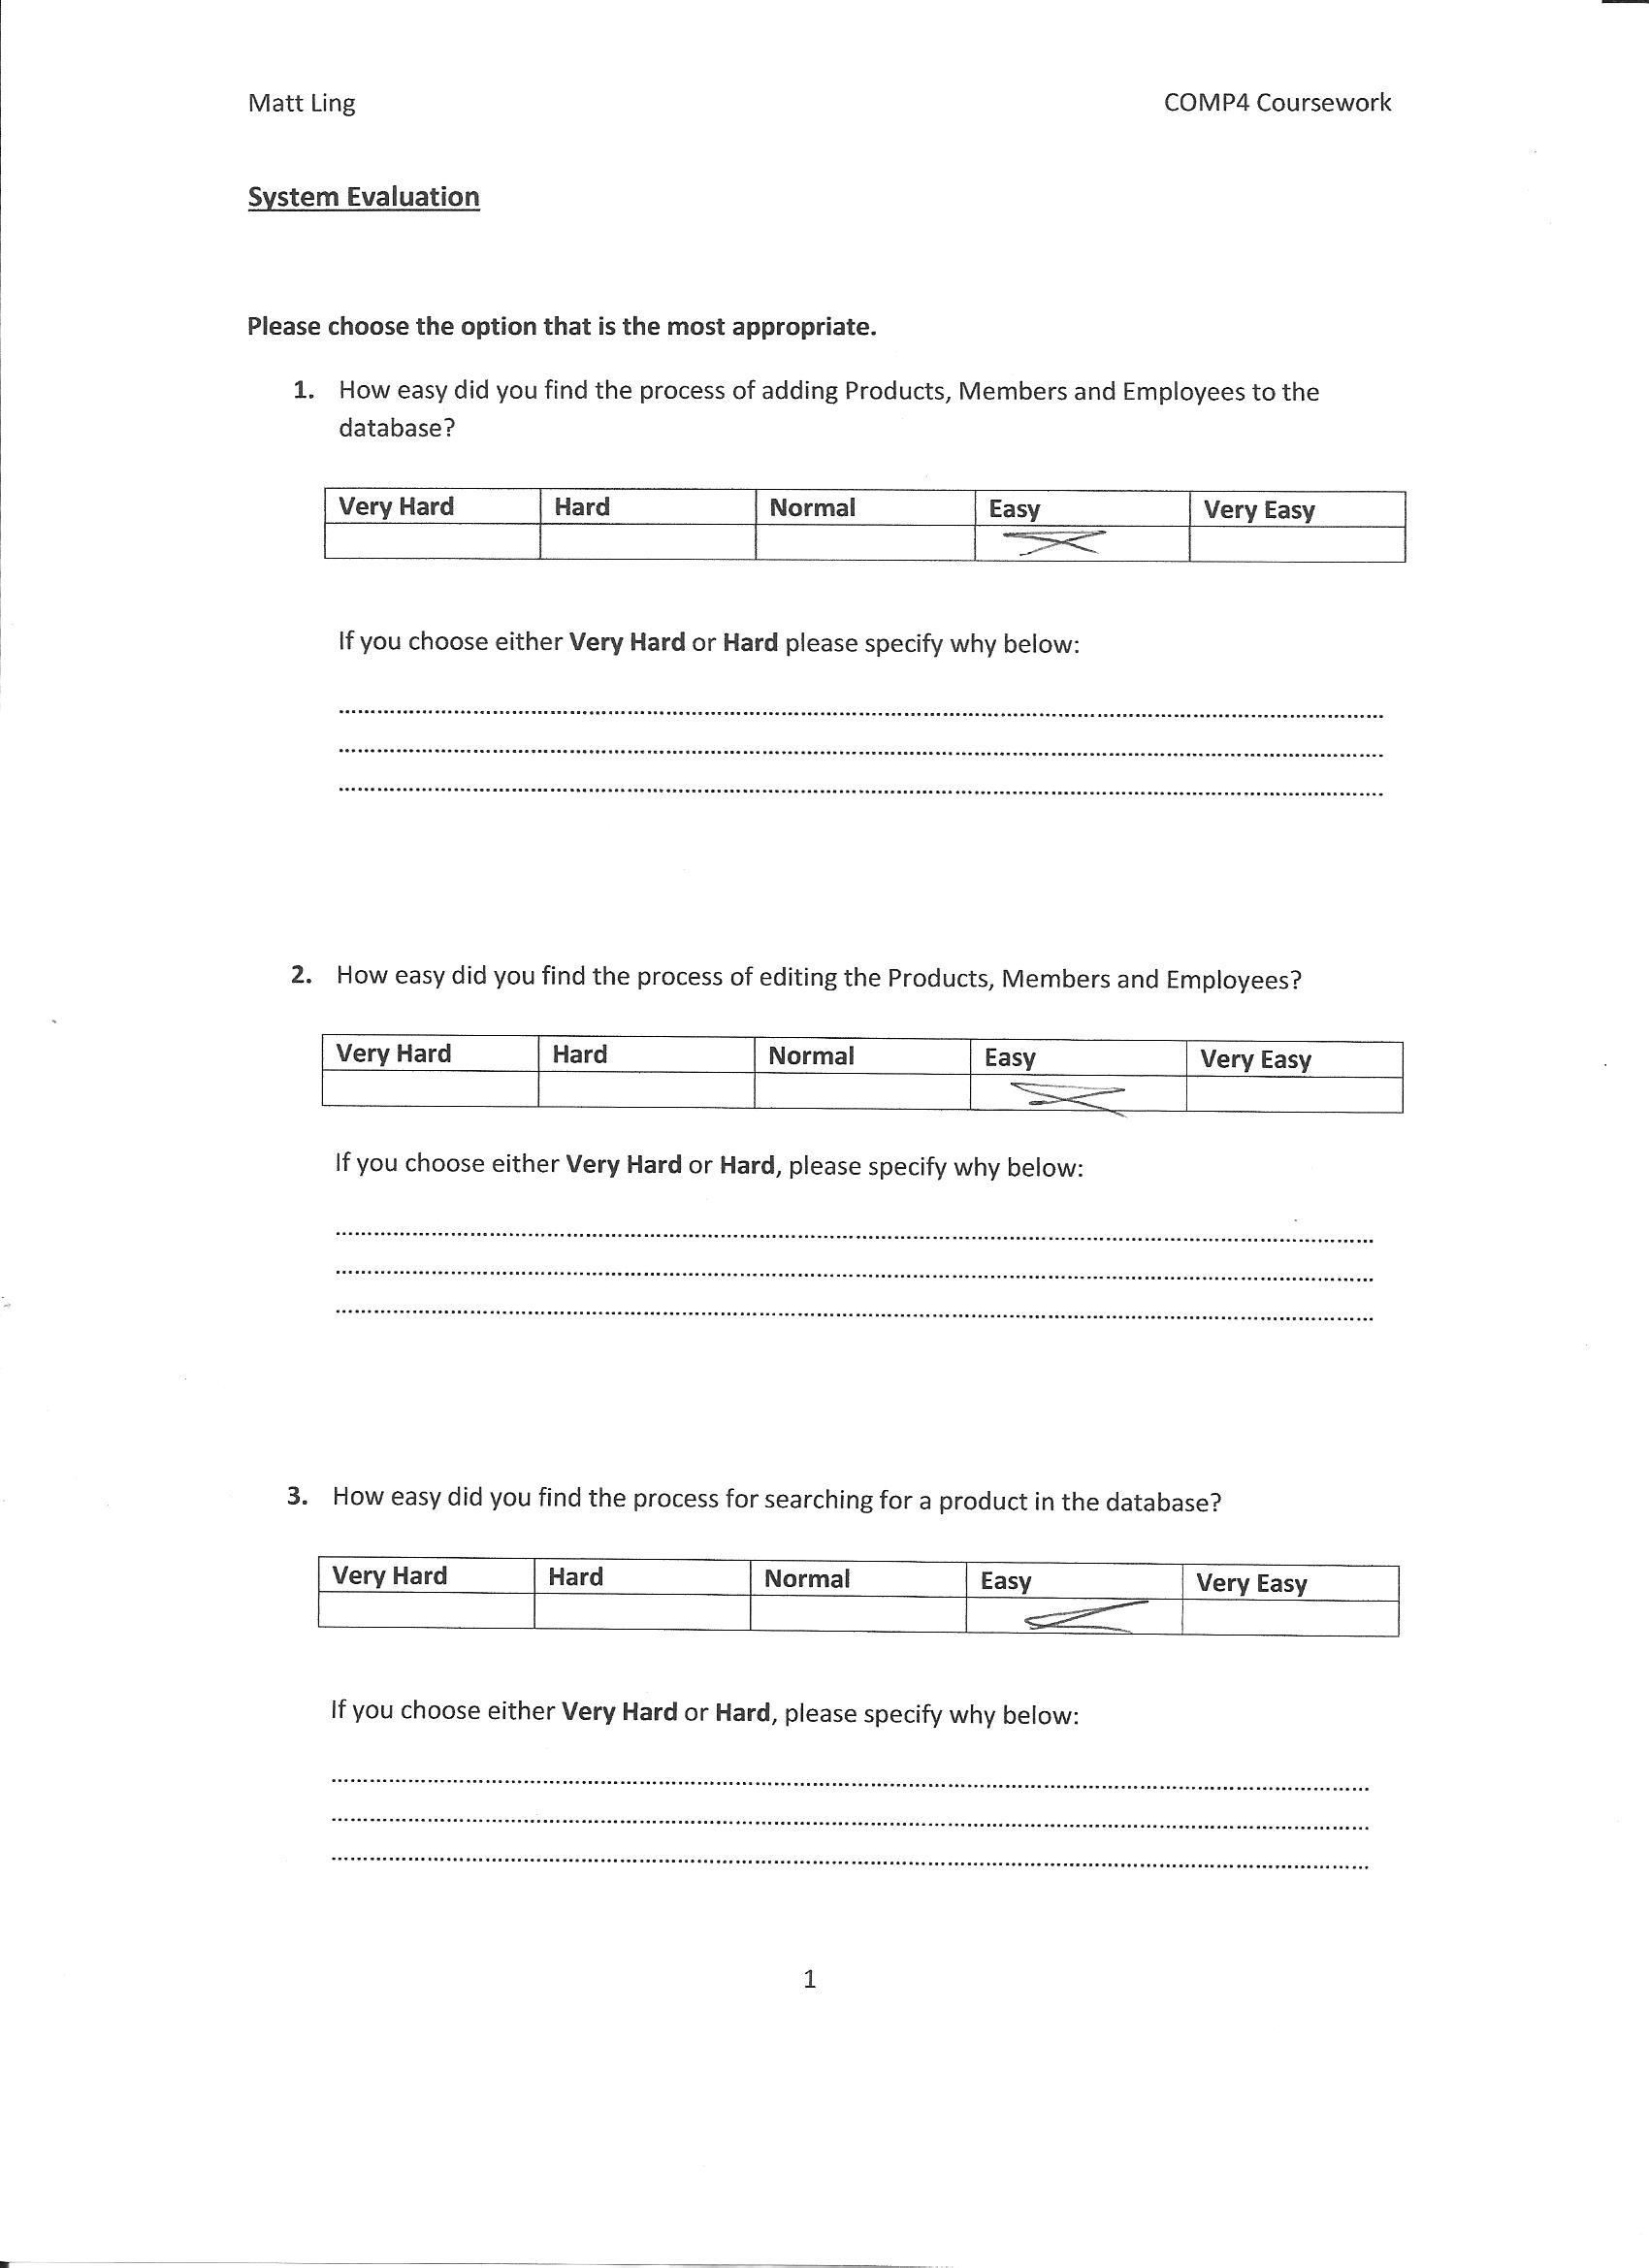
\includepdf{./EvaluationImages/questionaire-1-page-1.jpg}
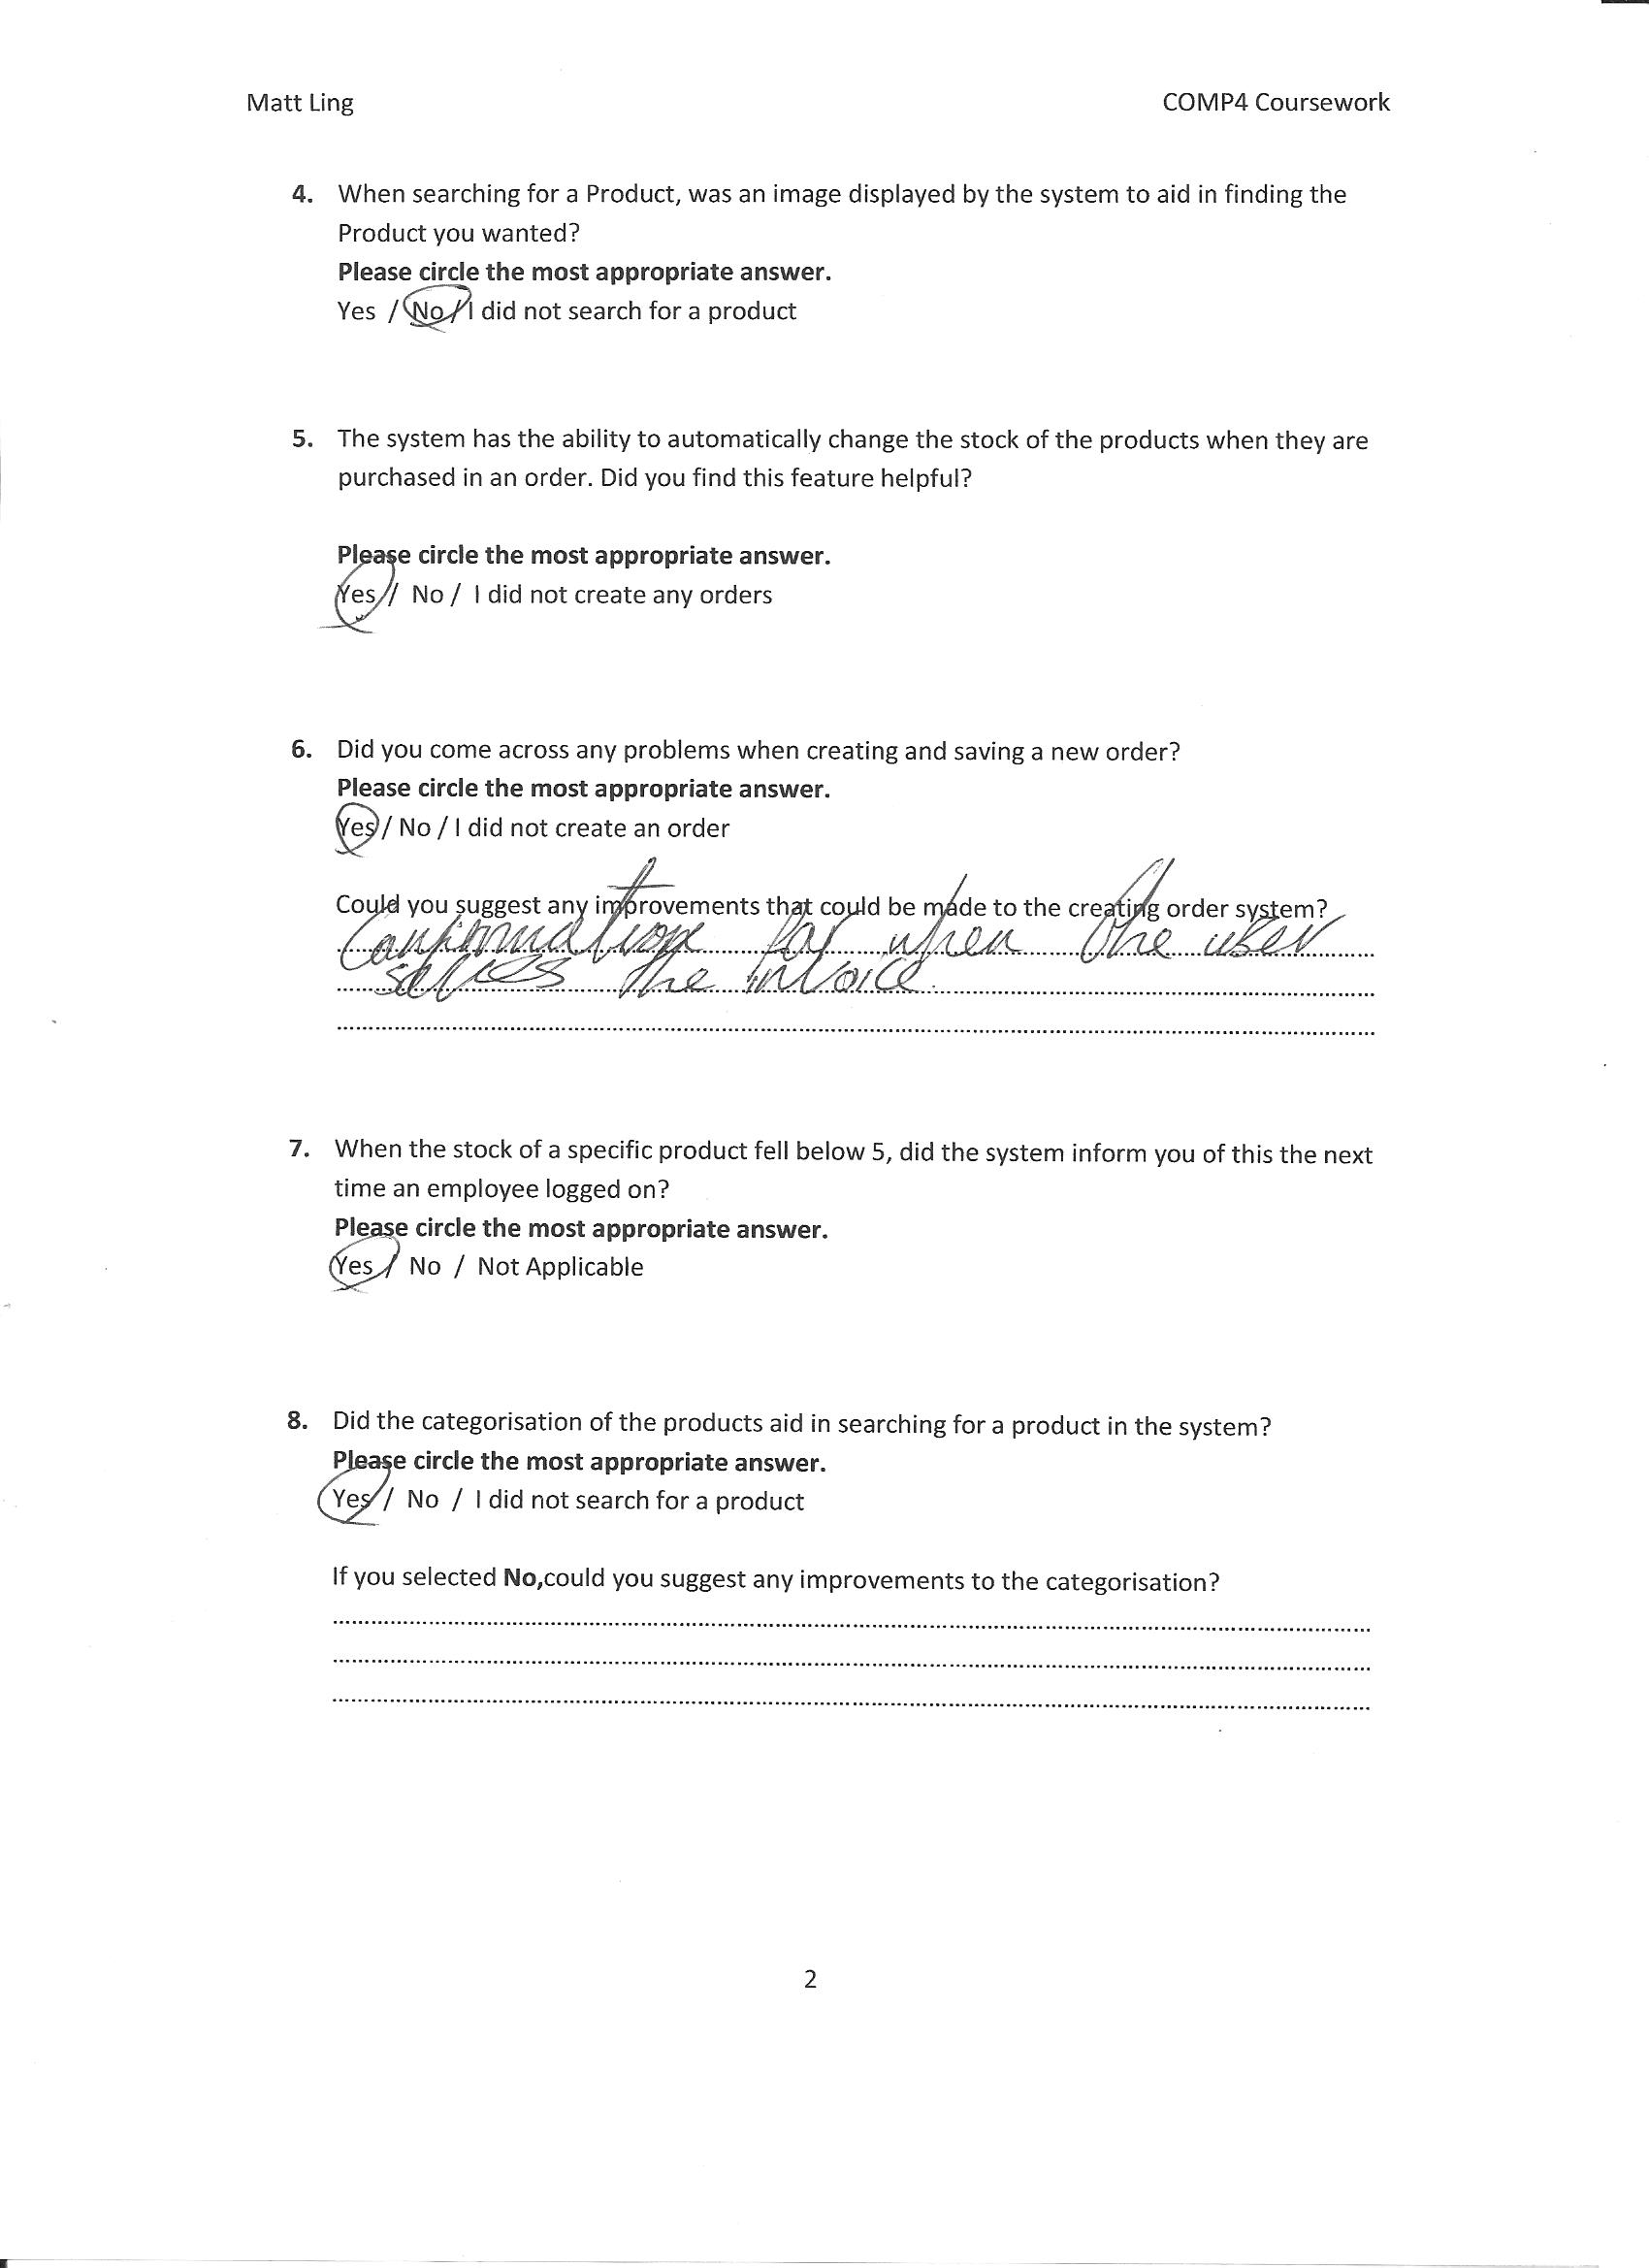
\includepdf{./EvaluationImages/questionaire-1-page-2.jpg}
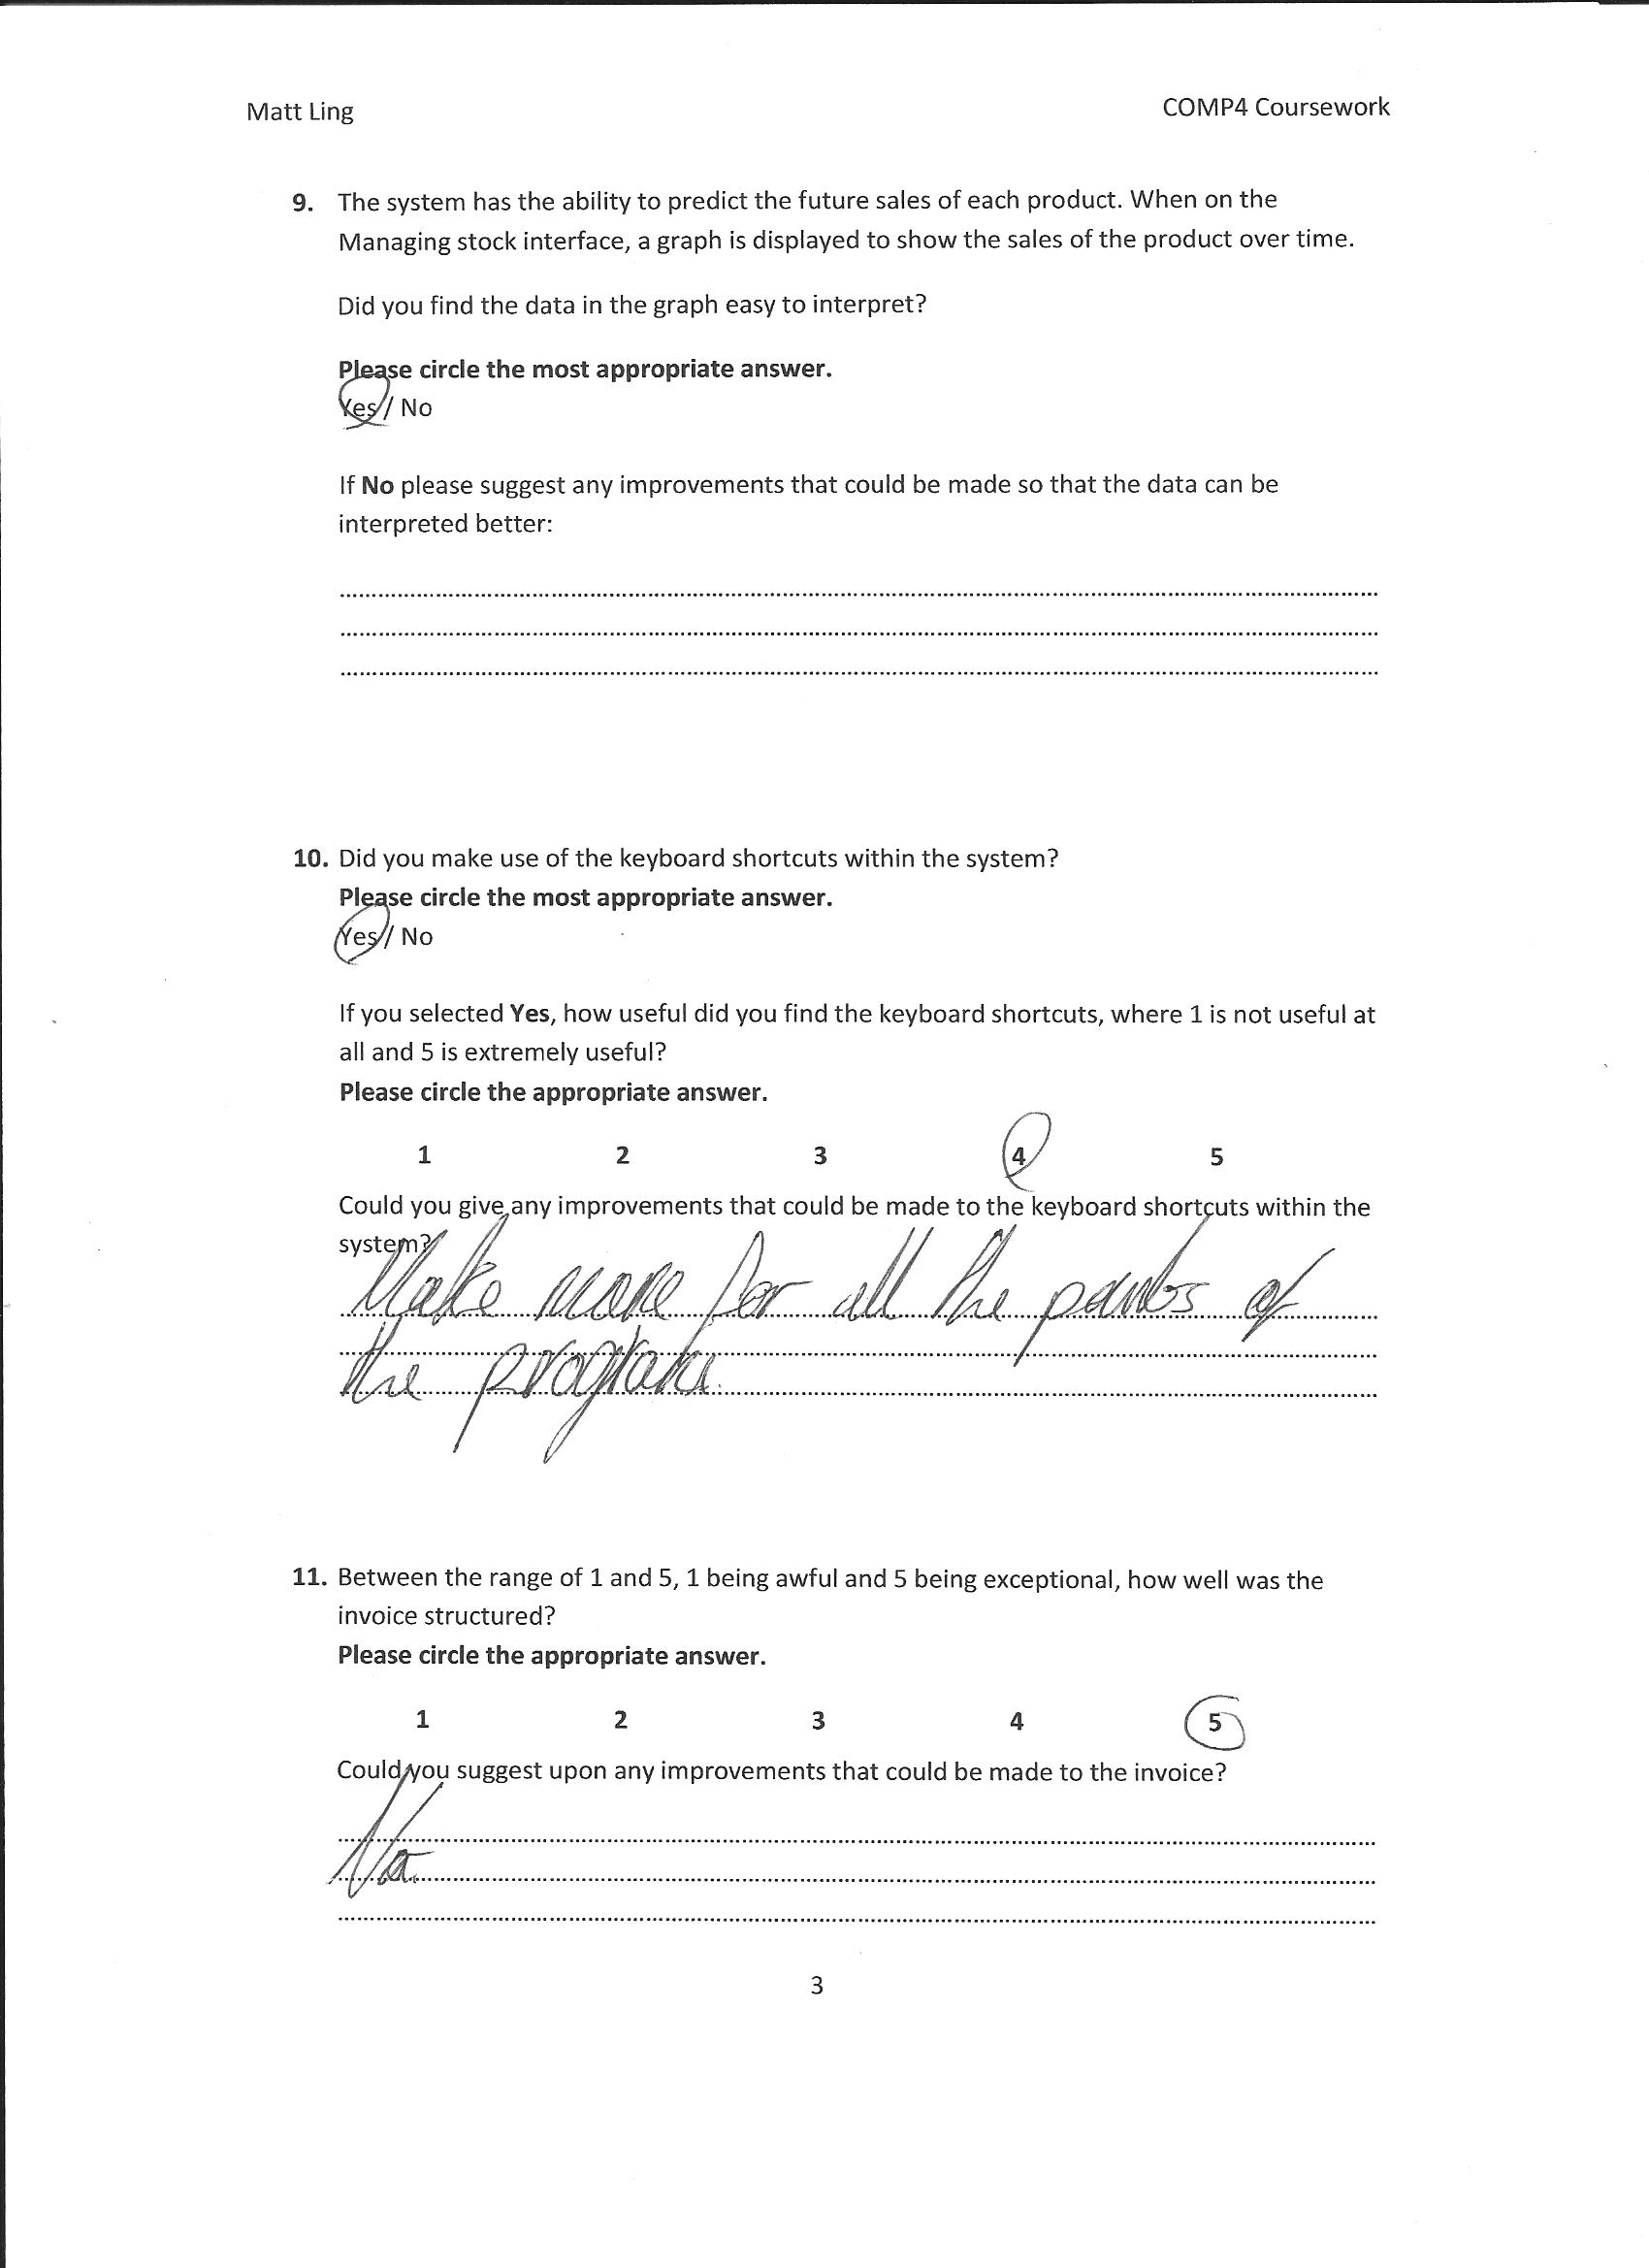
\includepdf{./EvaluationImages/questionaire-1-page-3.jpg}
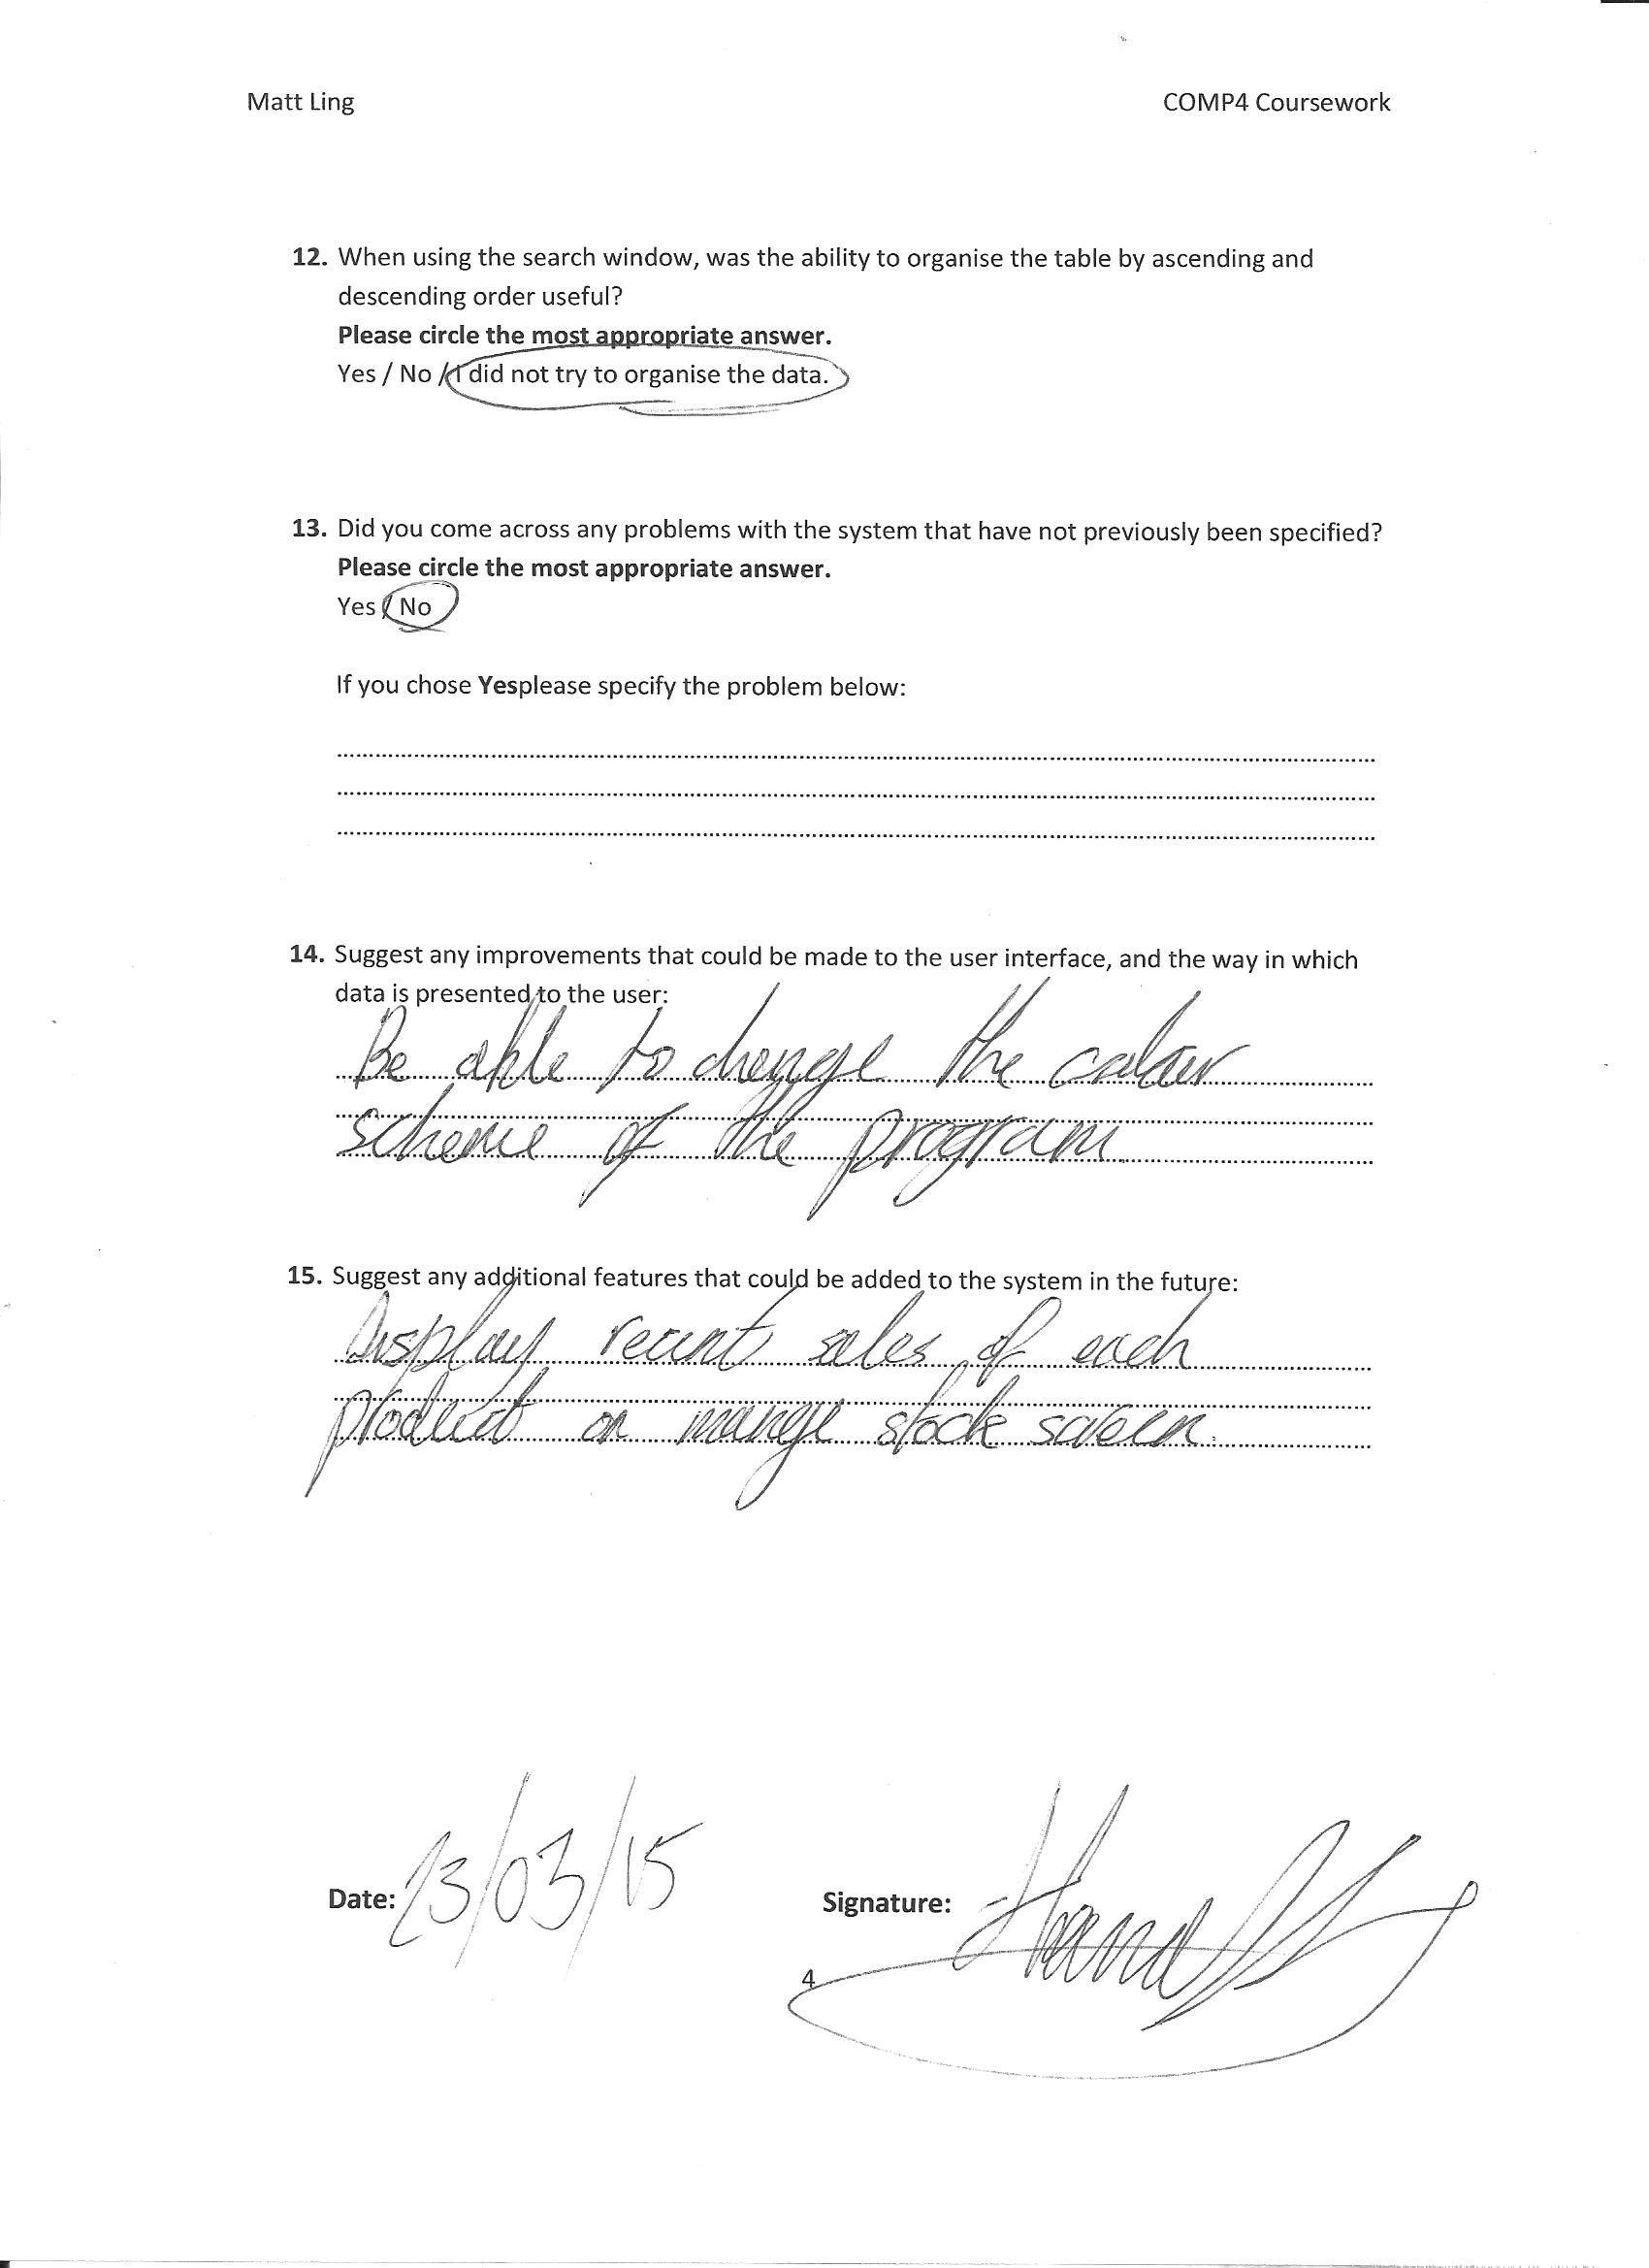
\includepdf{./EvaluationImages/questionaire-1-page-4.jpg}


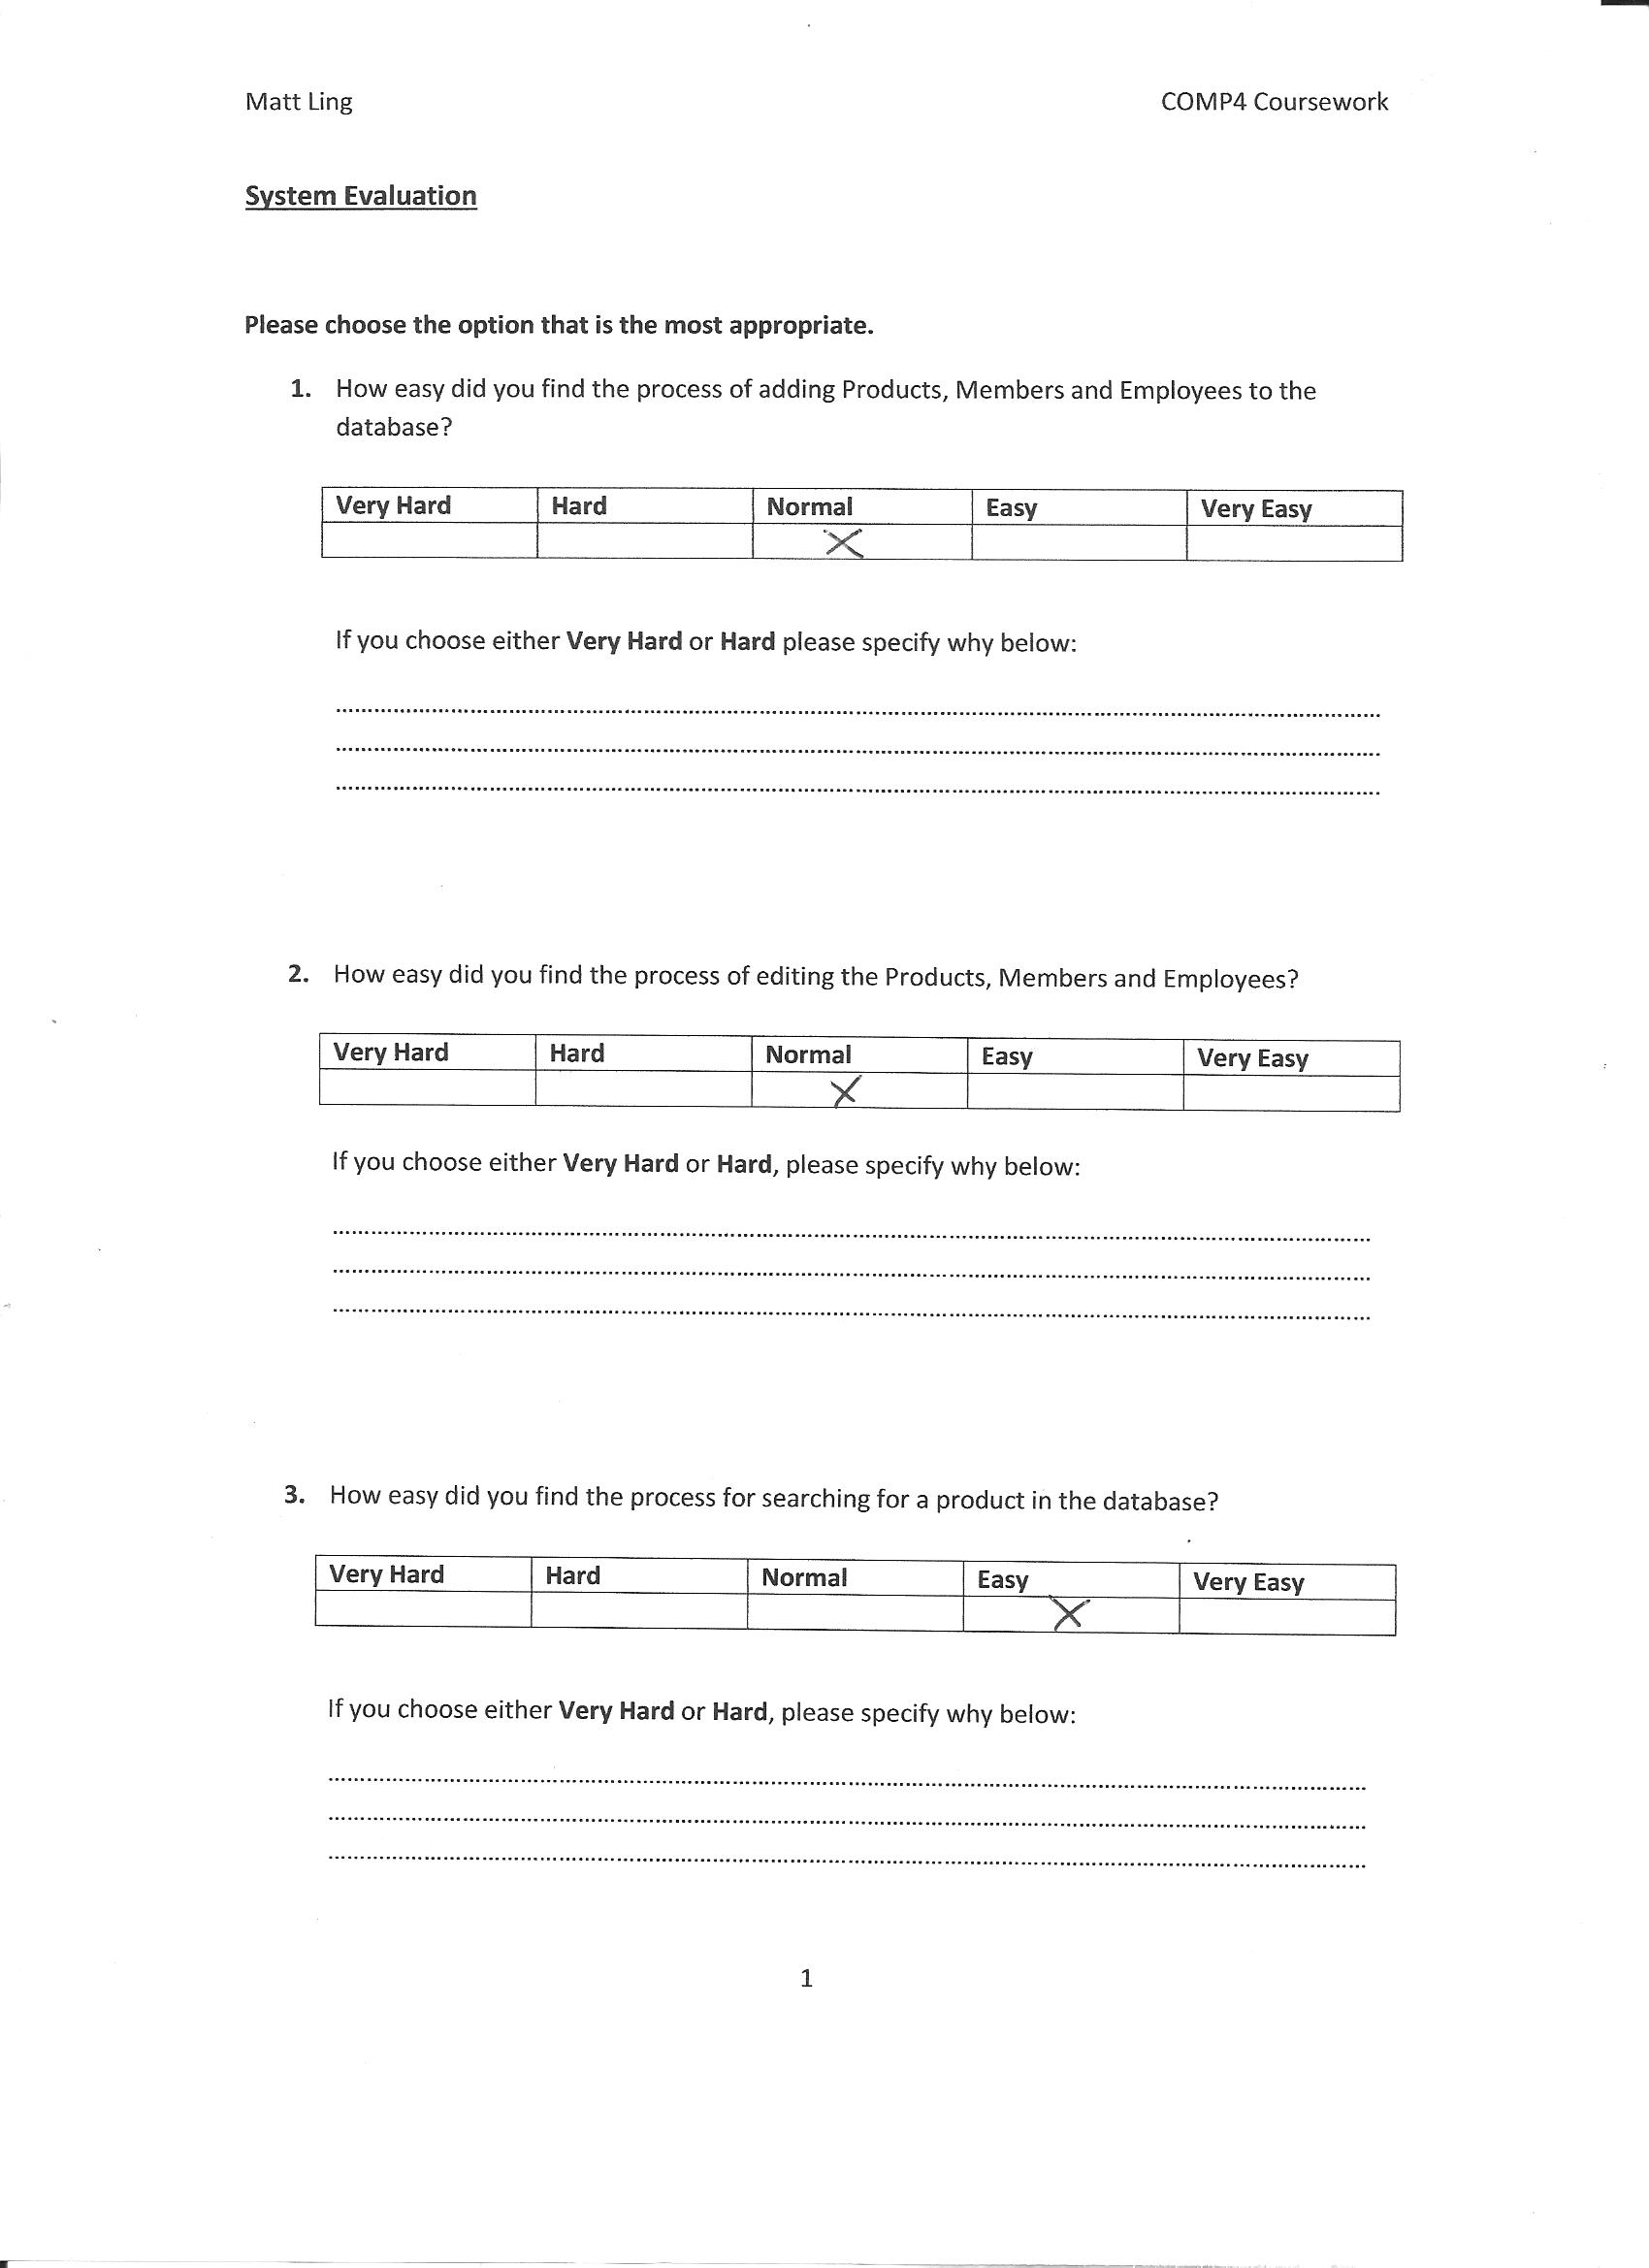
\includepdf{./EvaluationImages/questionaire-2-page-1.jpg}
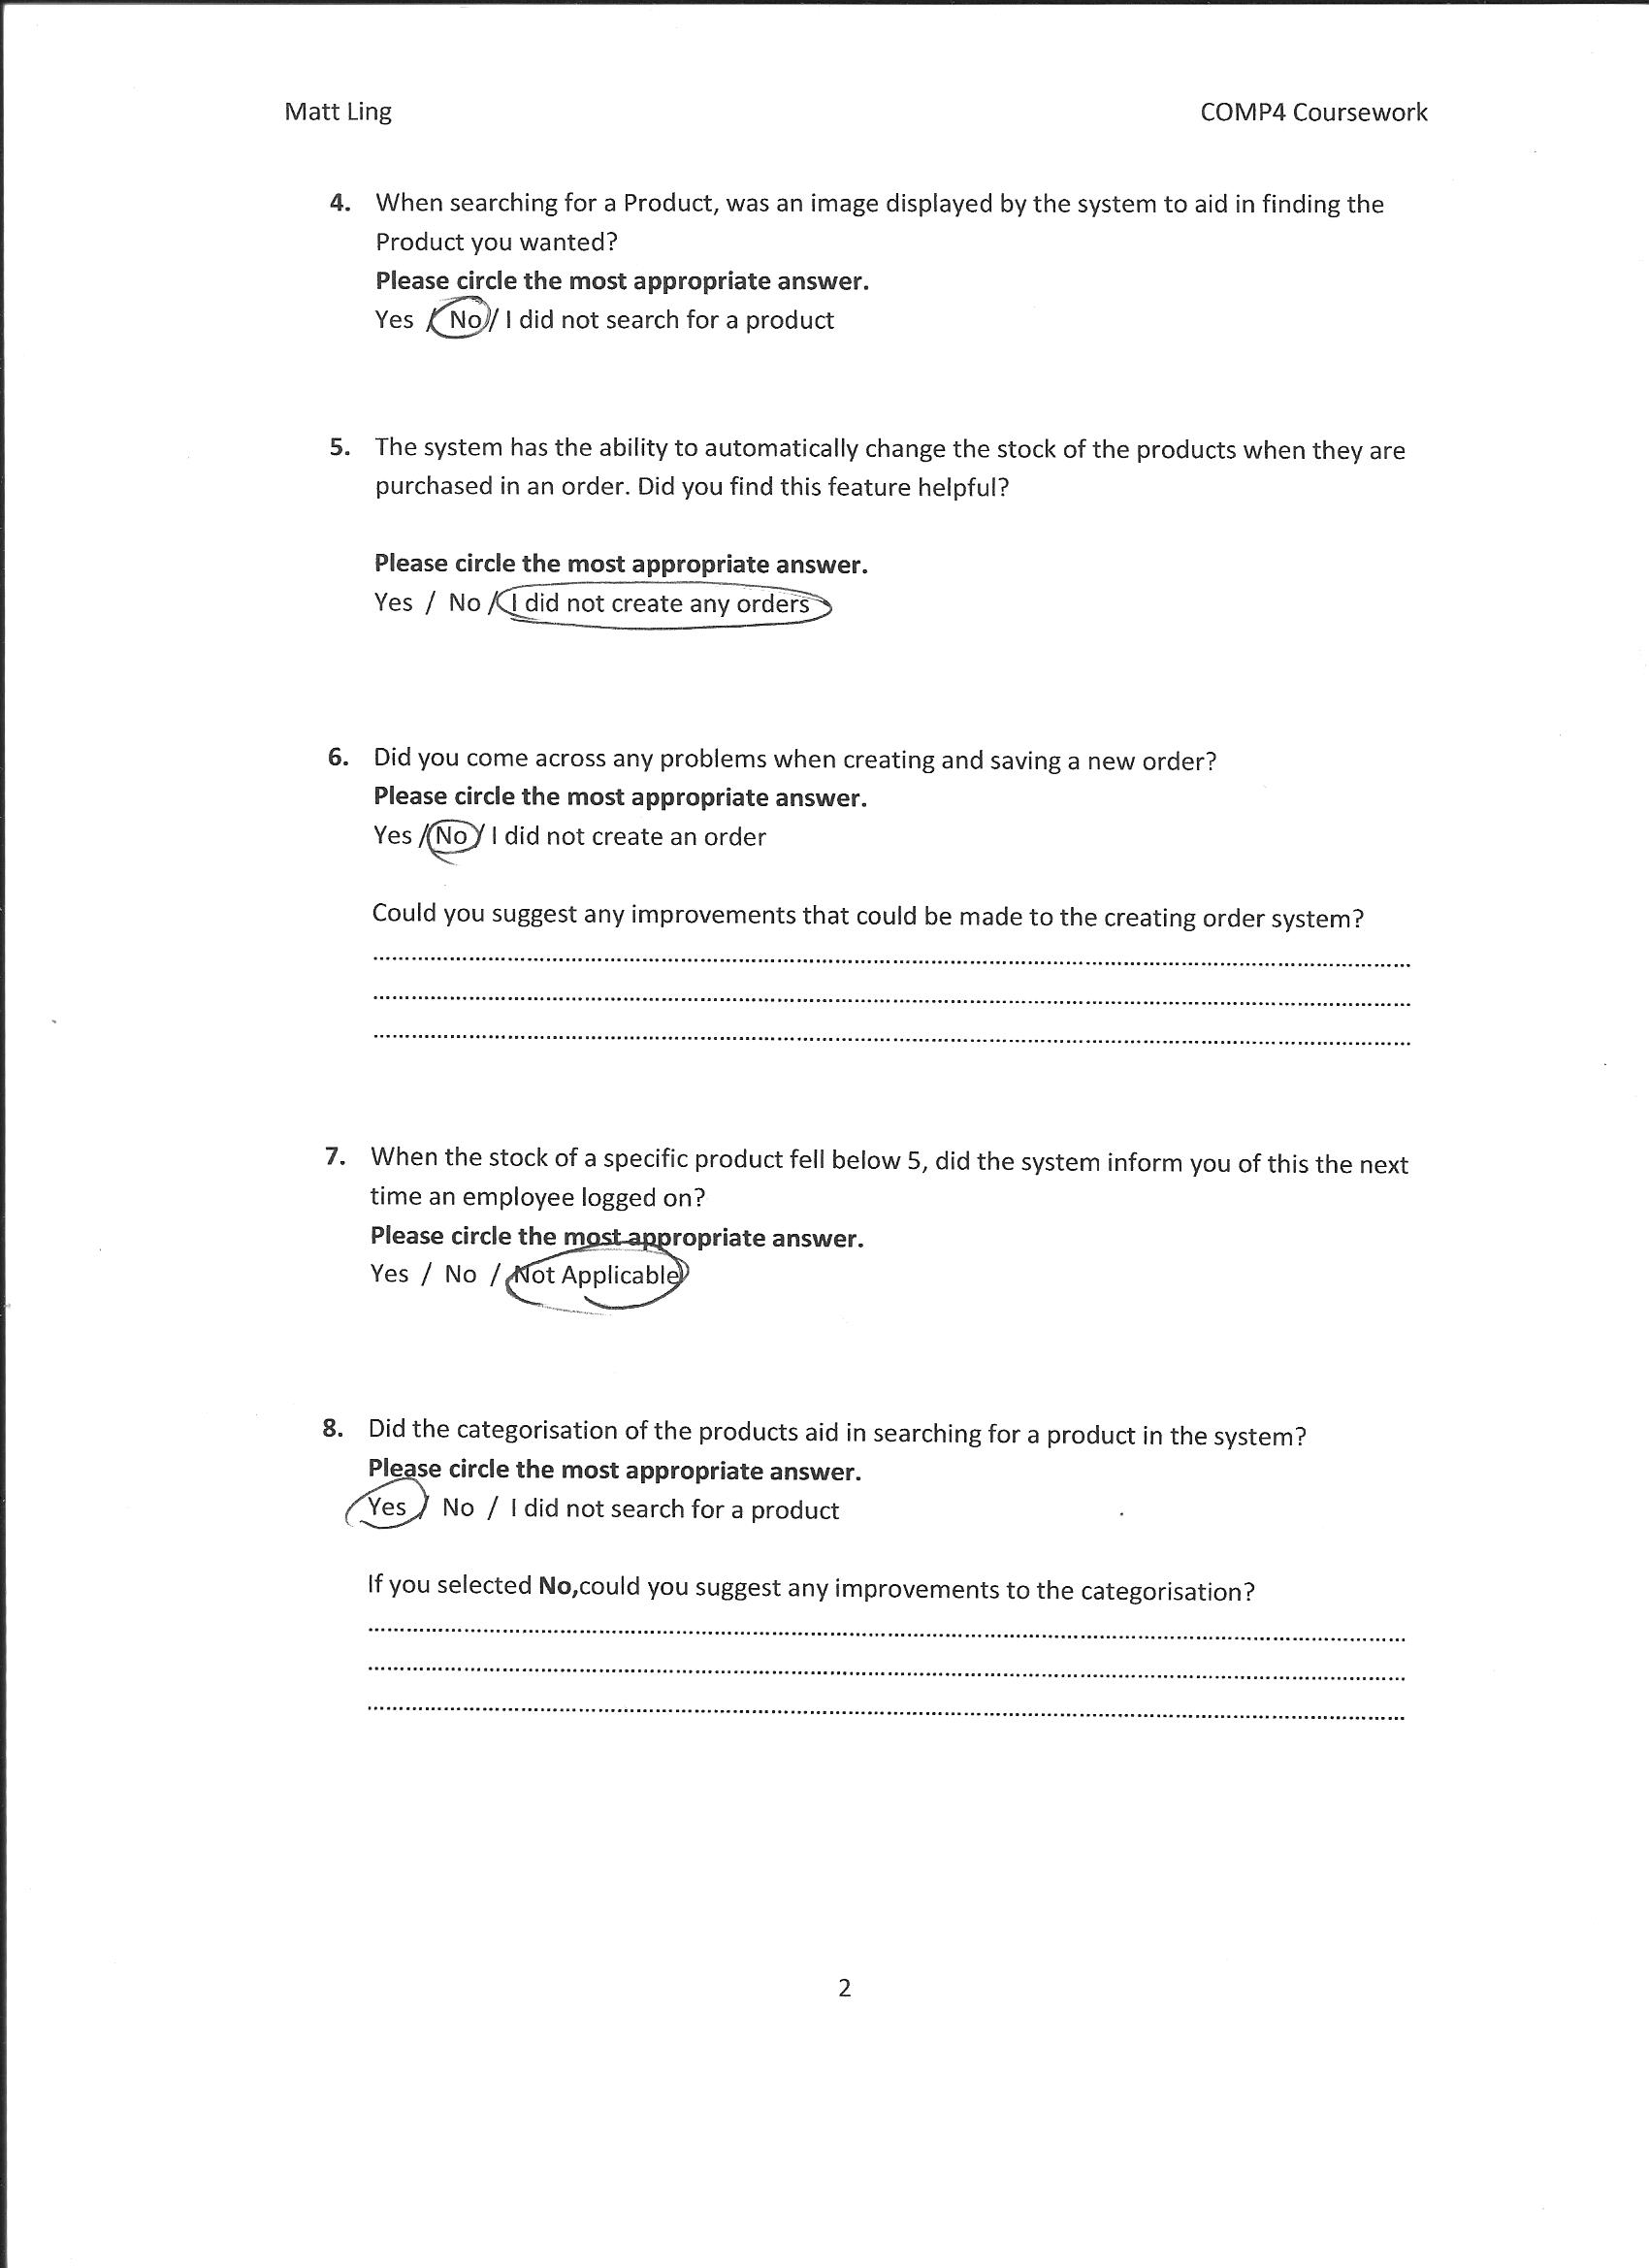
\includepdf{./EvaluationImages/questionaire-2-page-2.jpg}
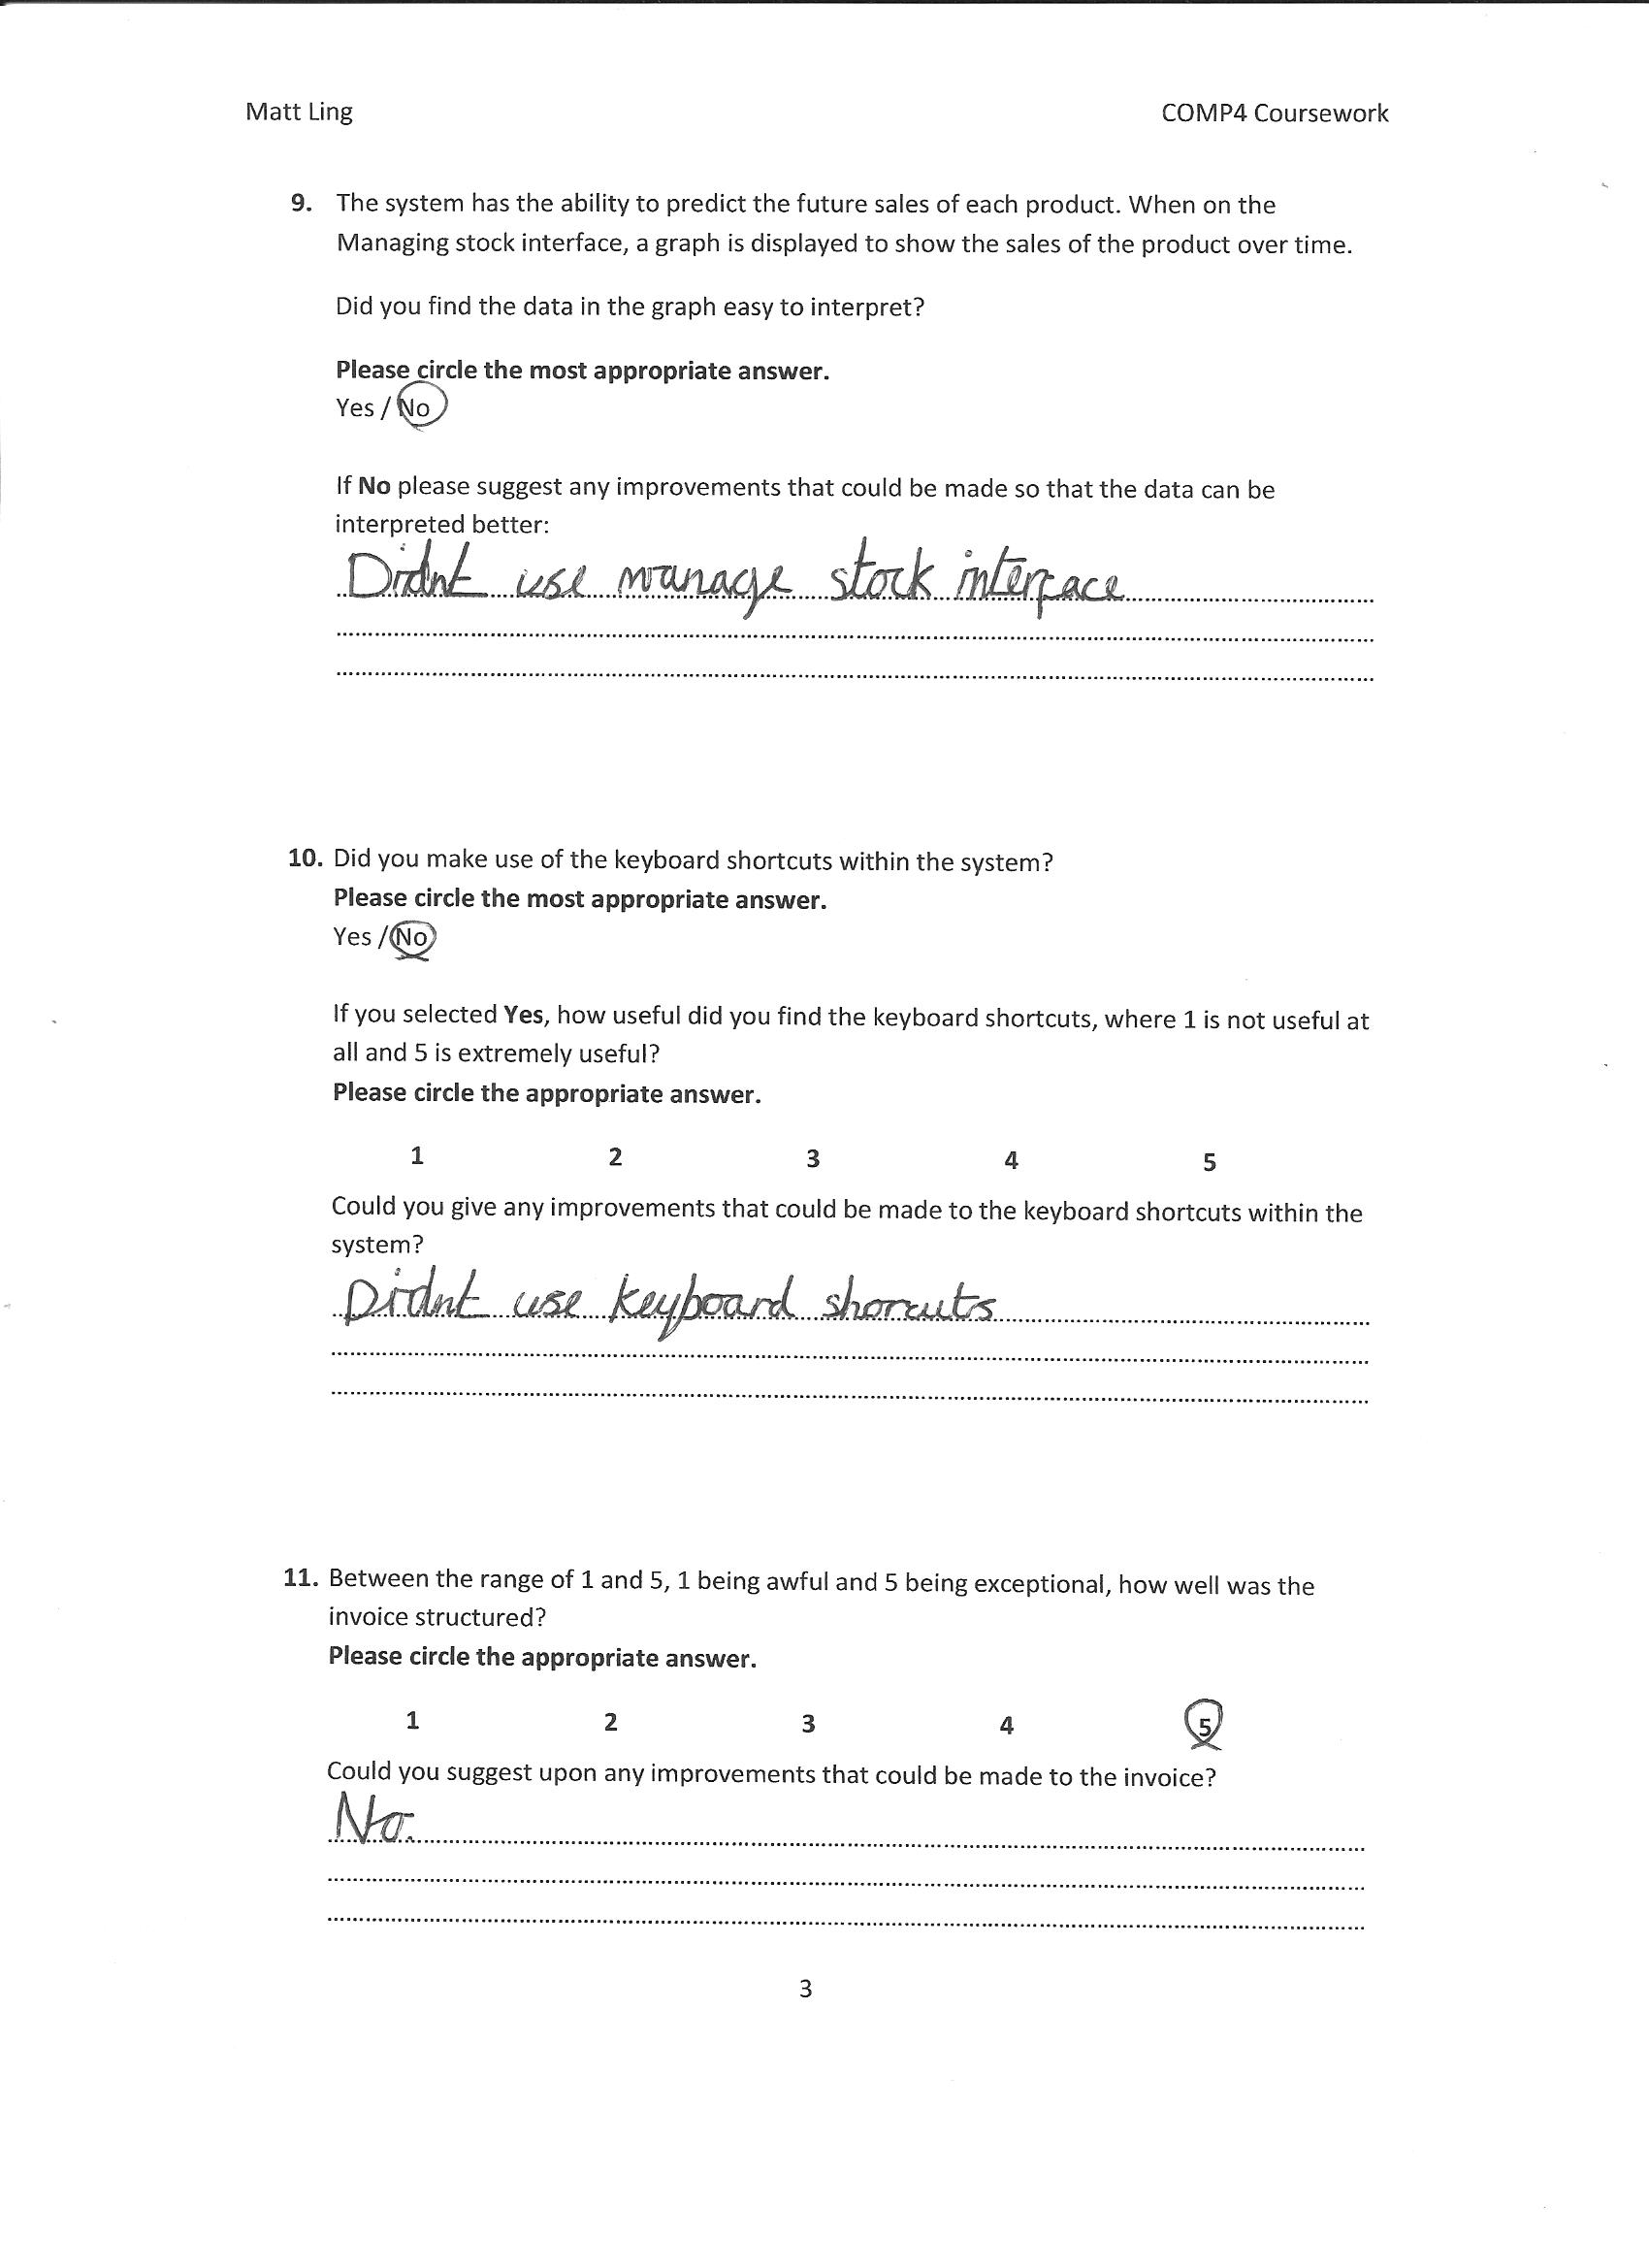
\includepdf{./EvaluationImages/questionaire-2-page-3.jpg}
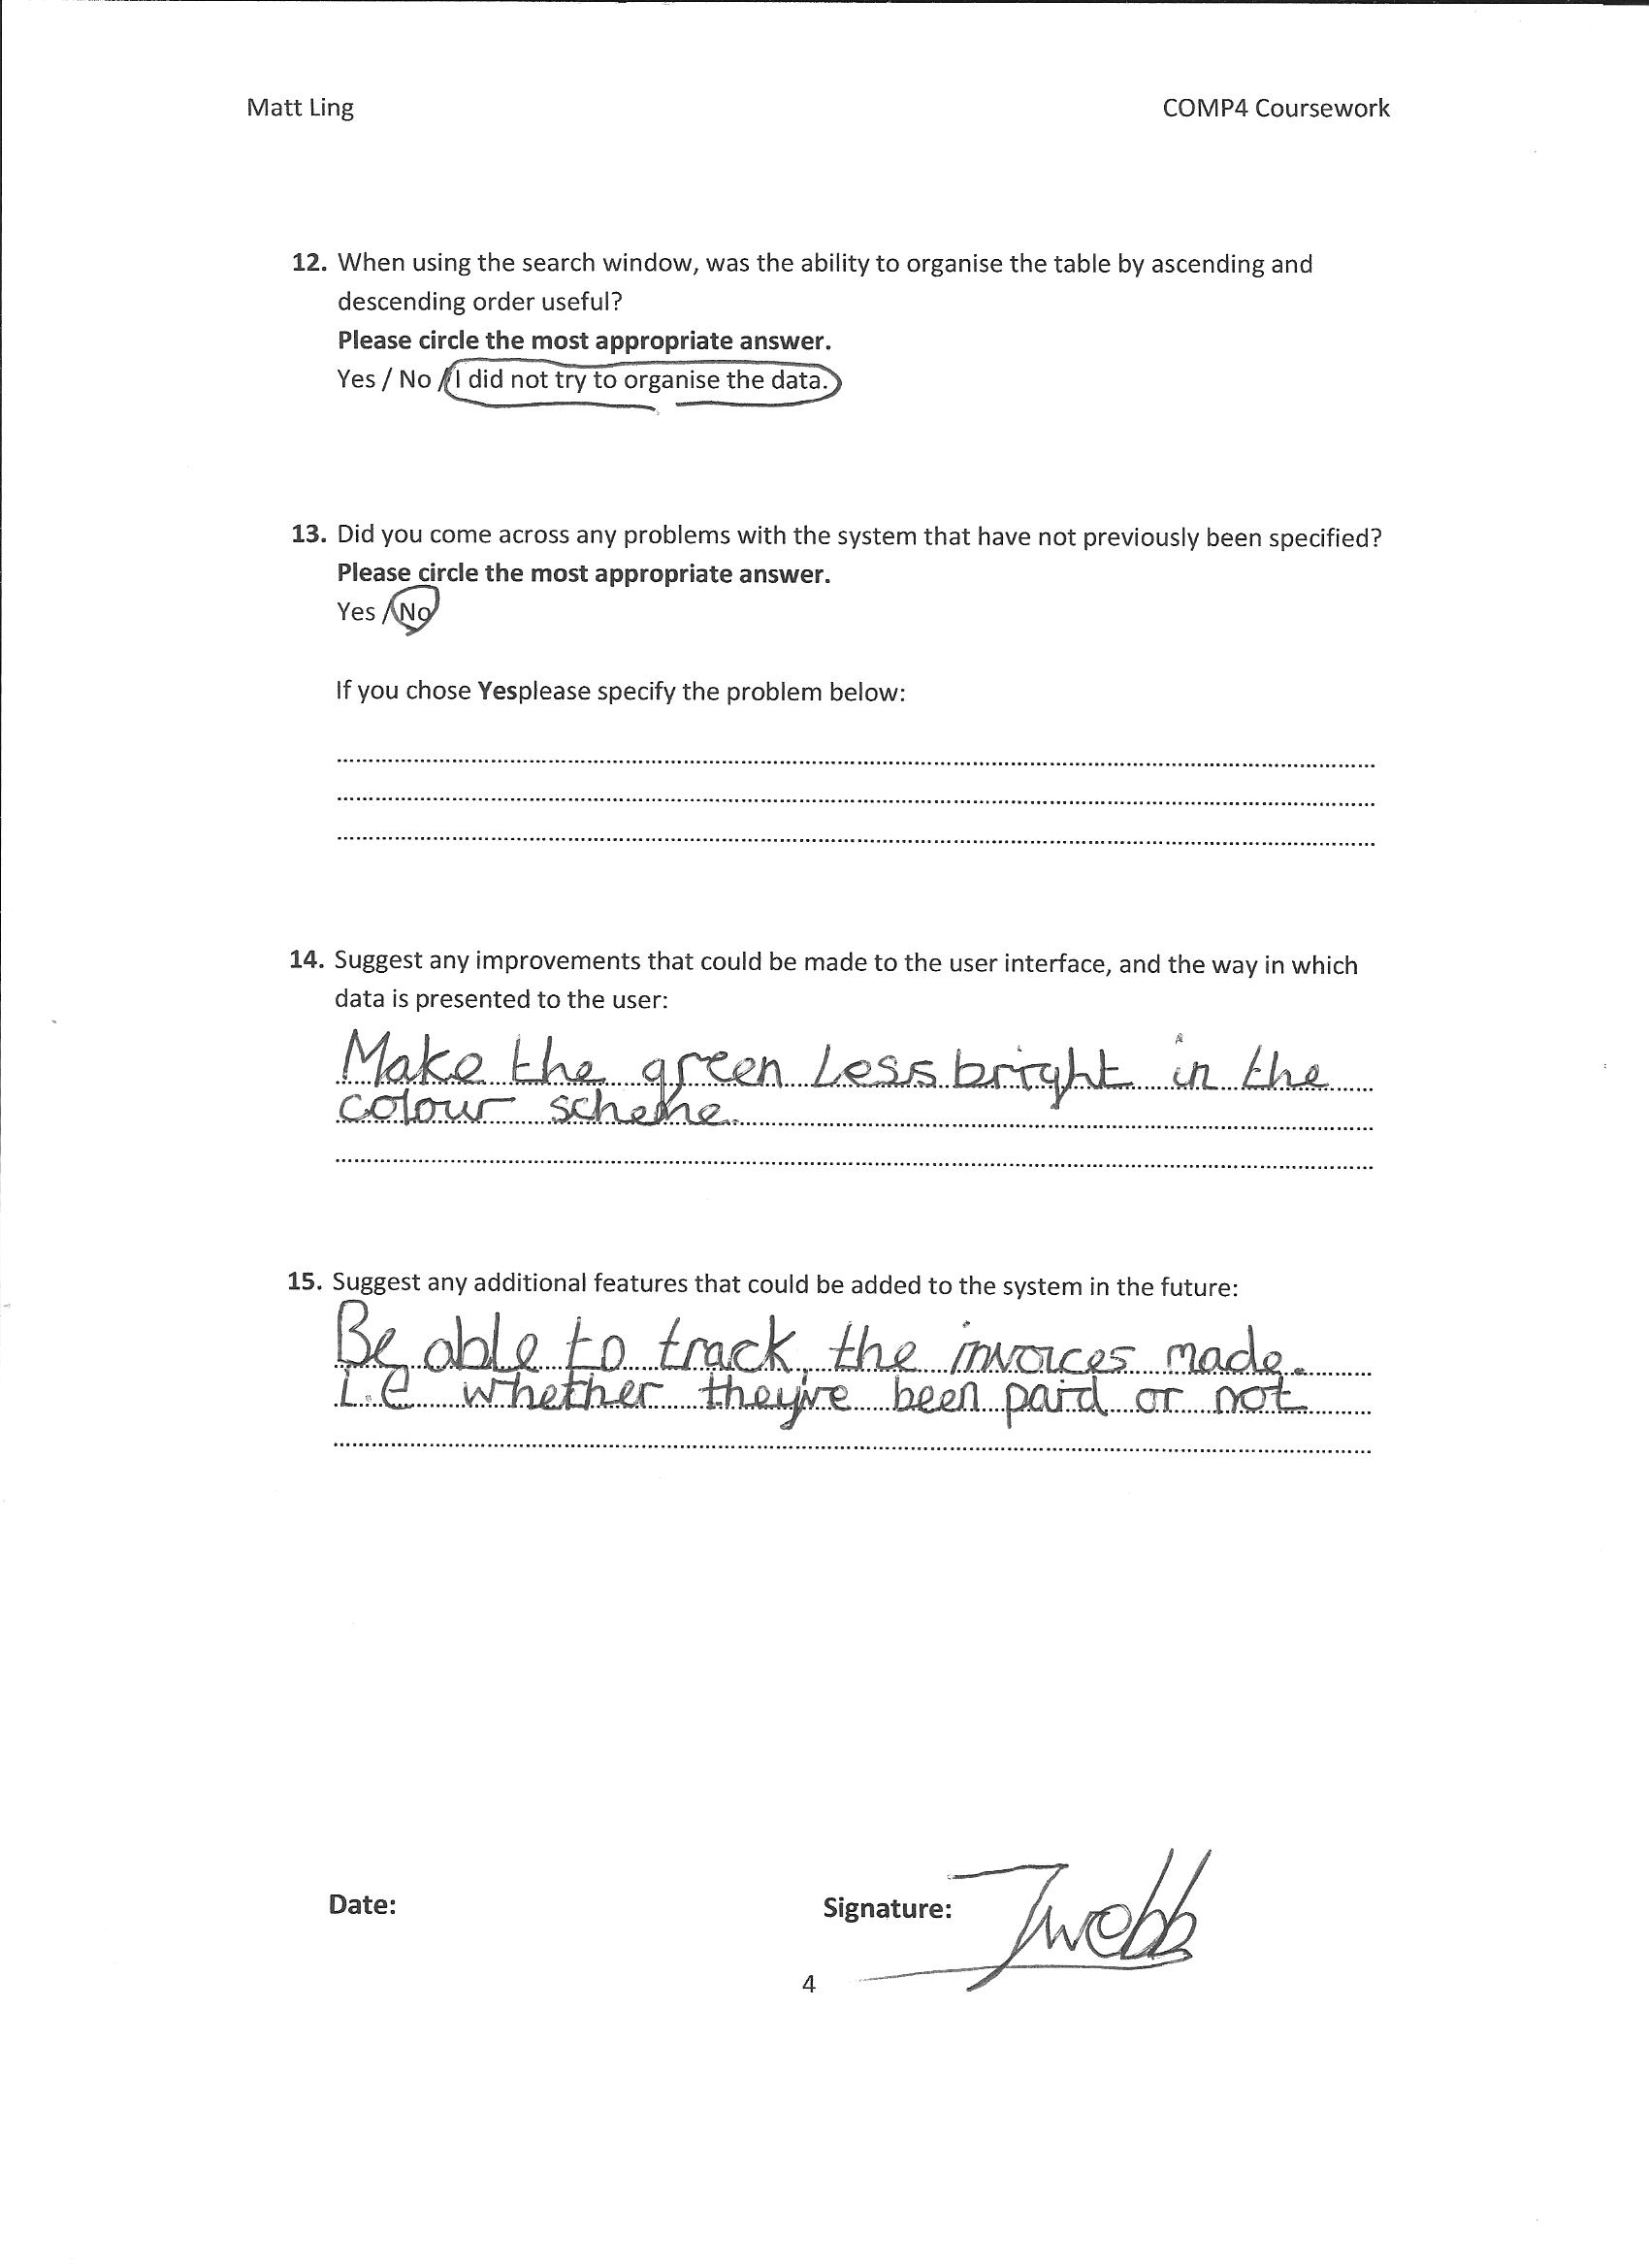
\includepdf{./EvaluationImages/questionaire-2-page-4.jpg}

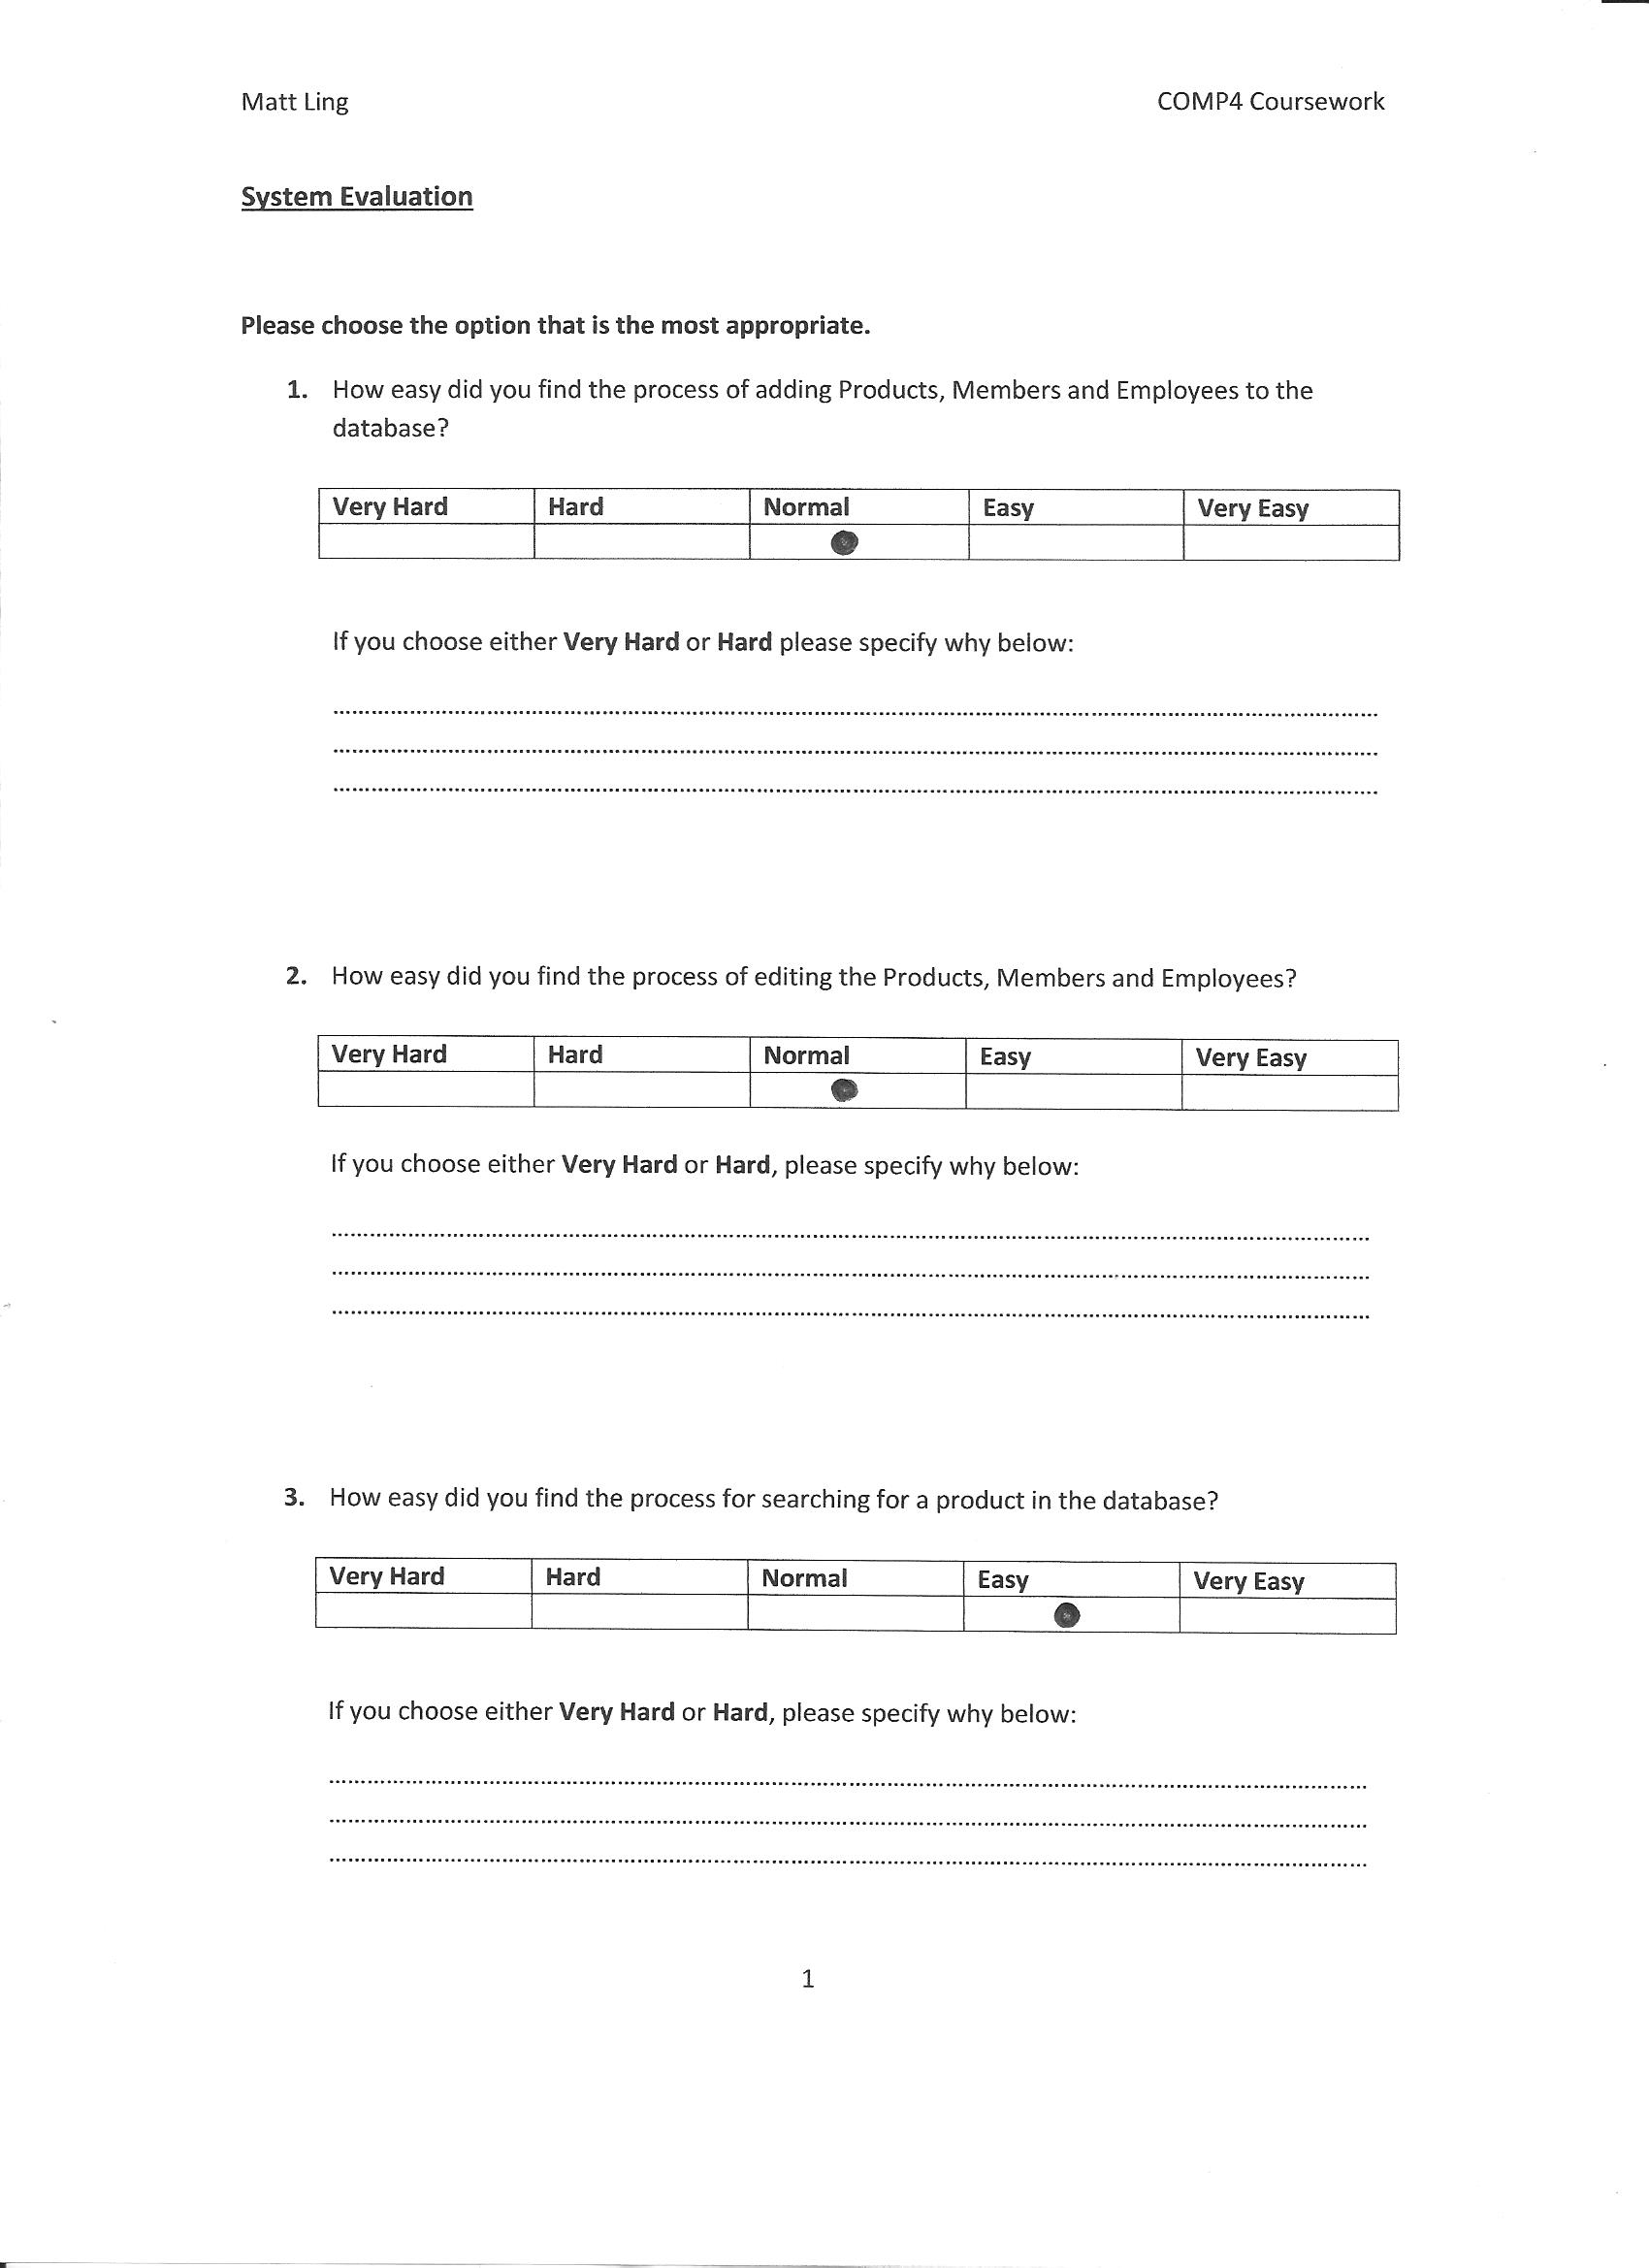
\includepdf{./EvaluationImages/questionaire-3-page-1.jpg}
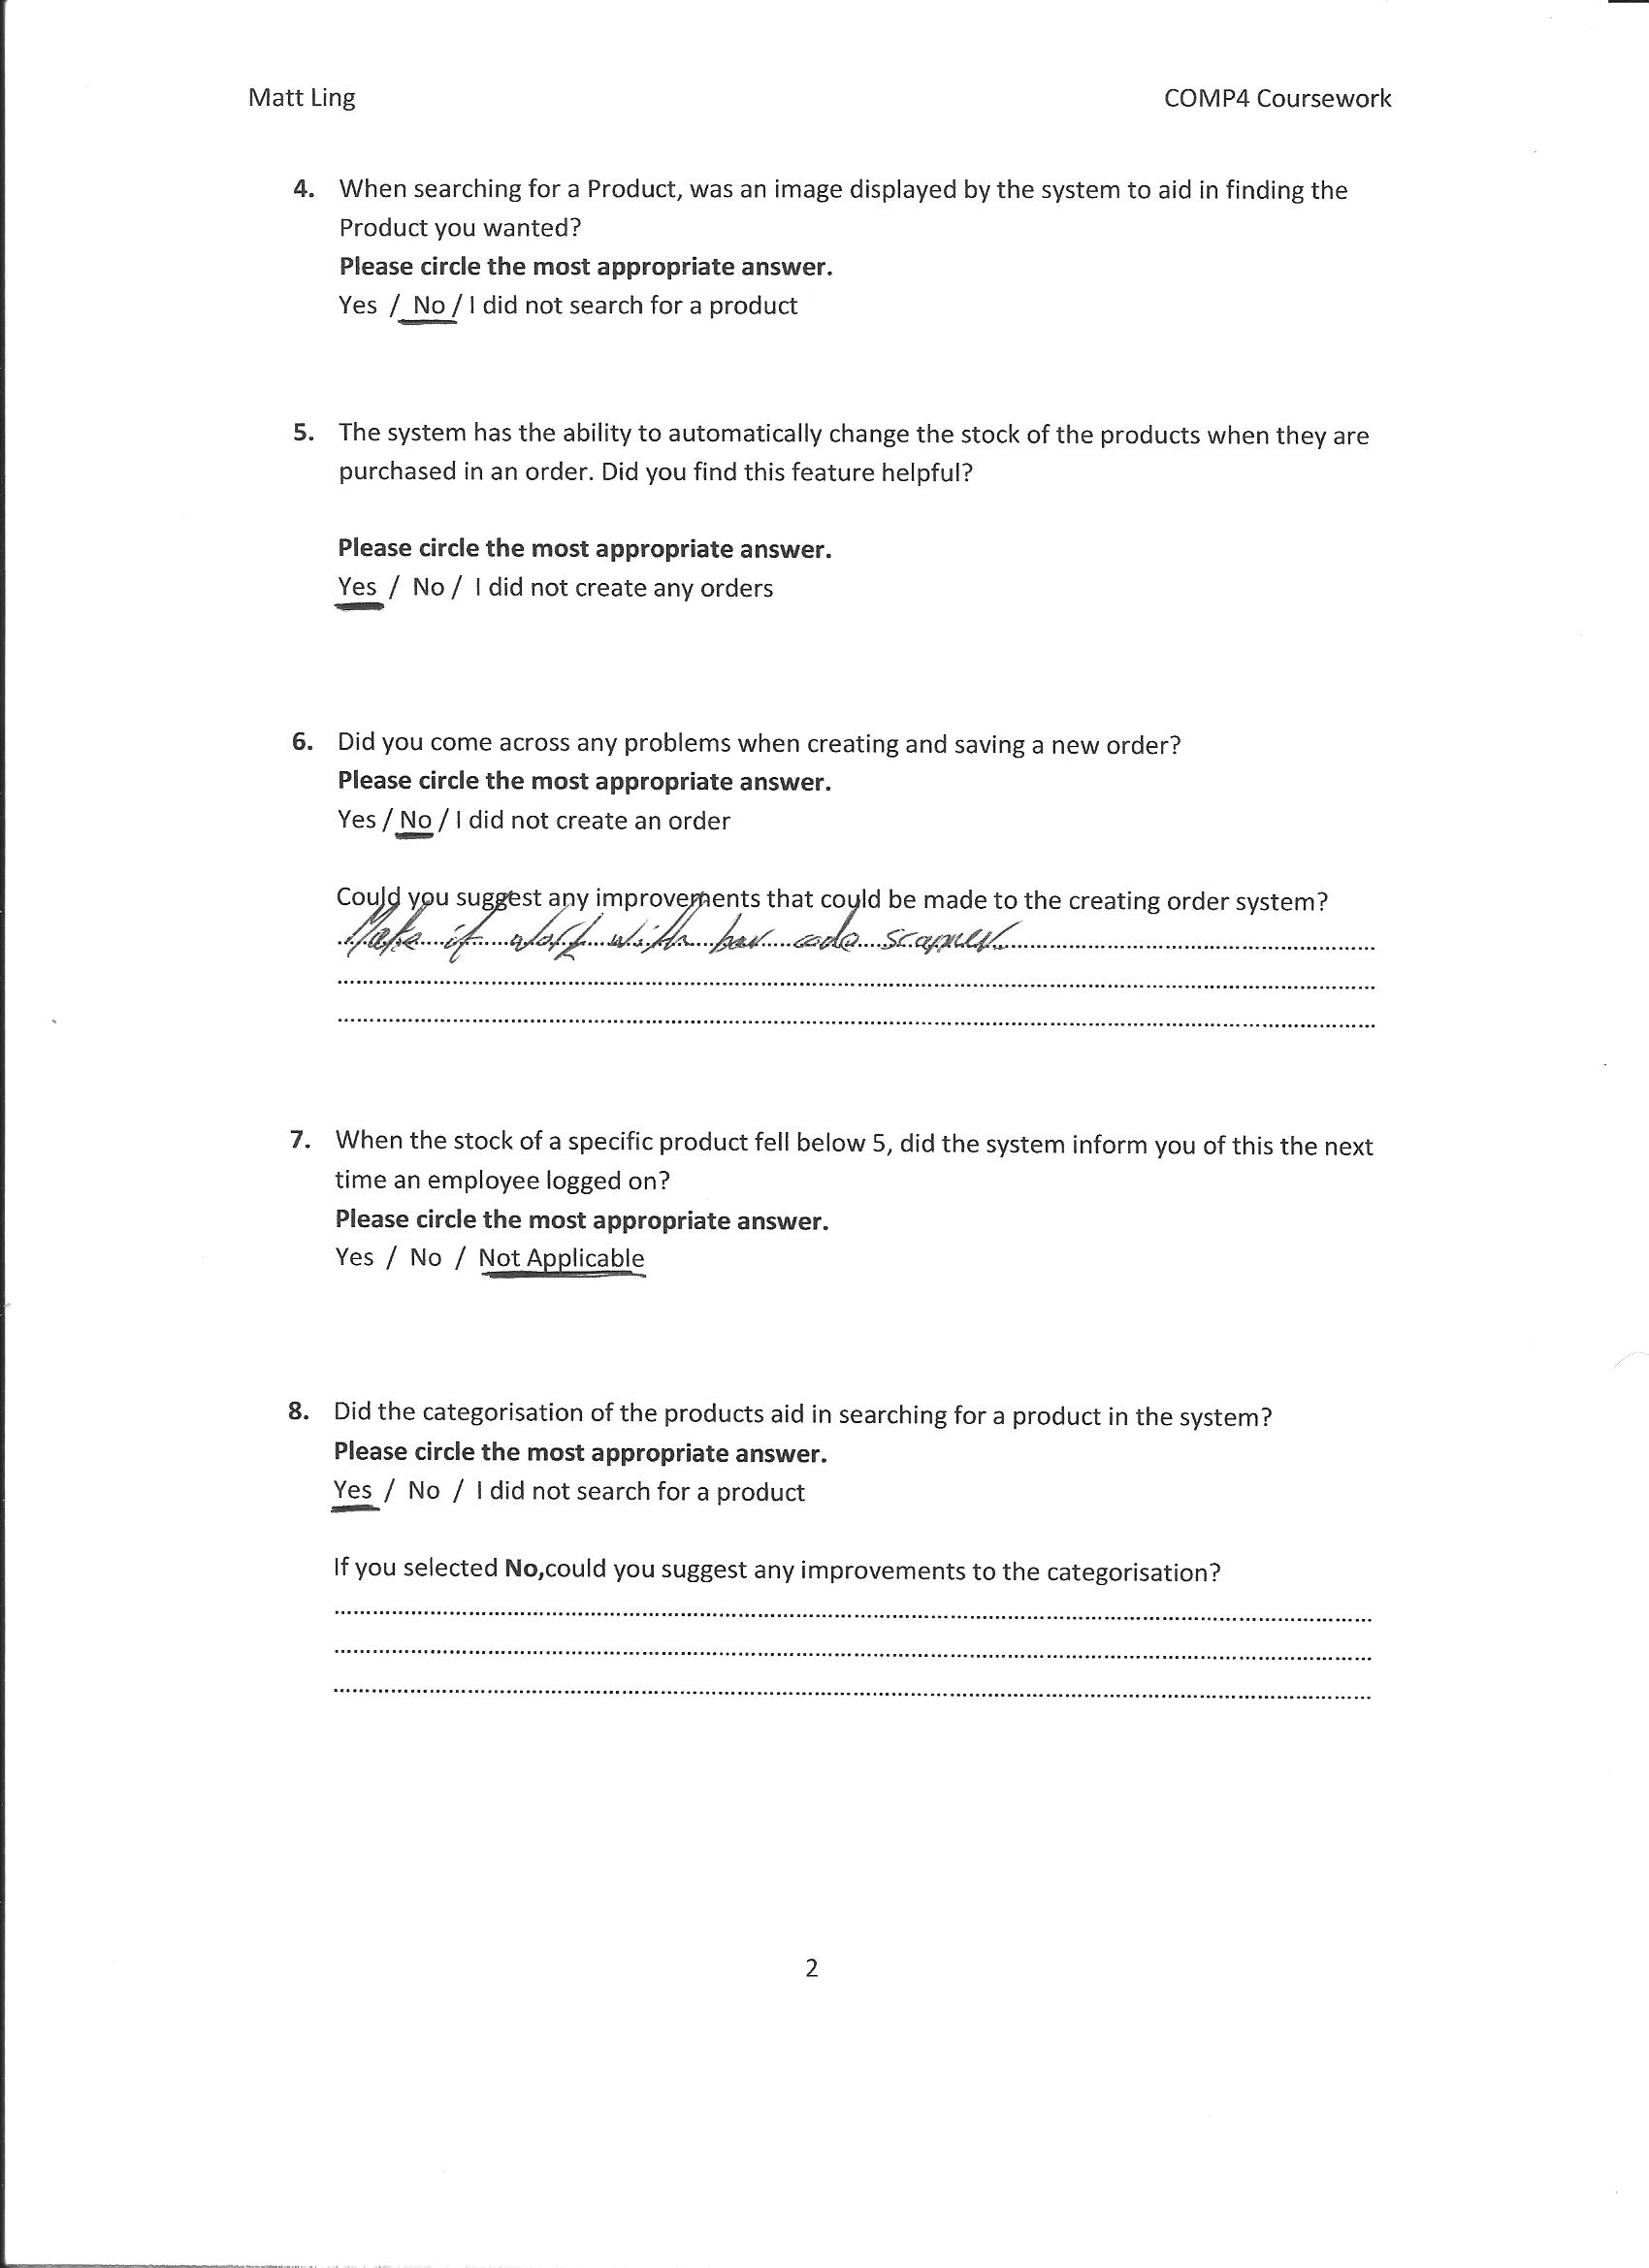
\includepdf{./EvaluationImages/questionaire-3-page-2.jpg}
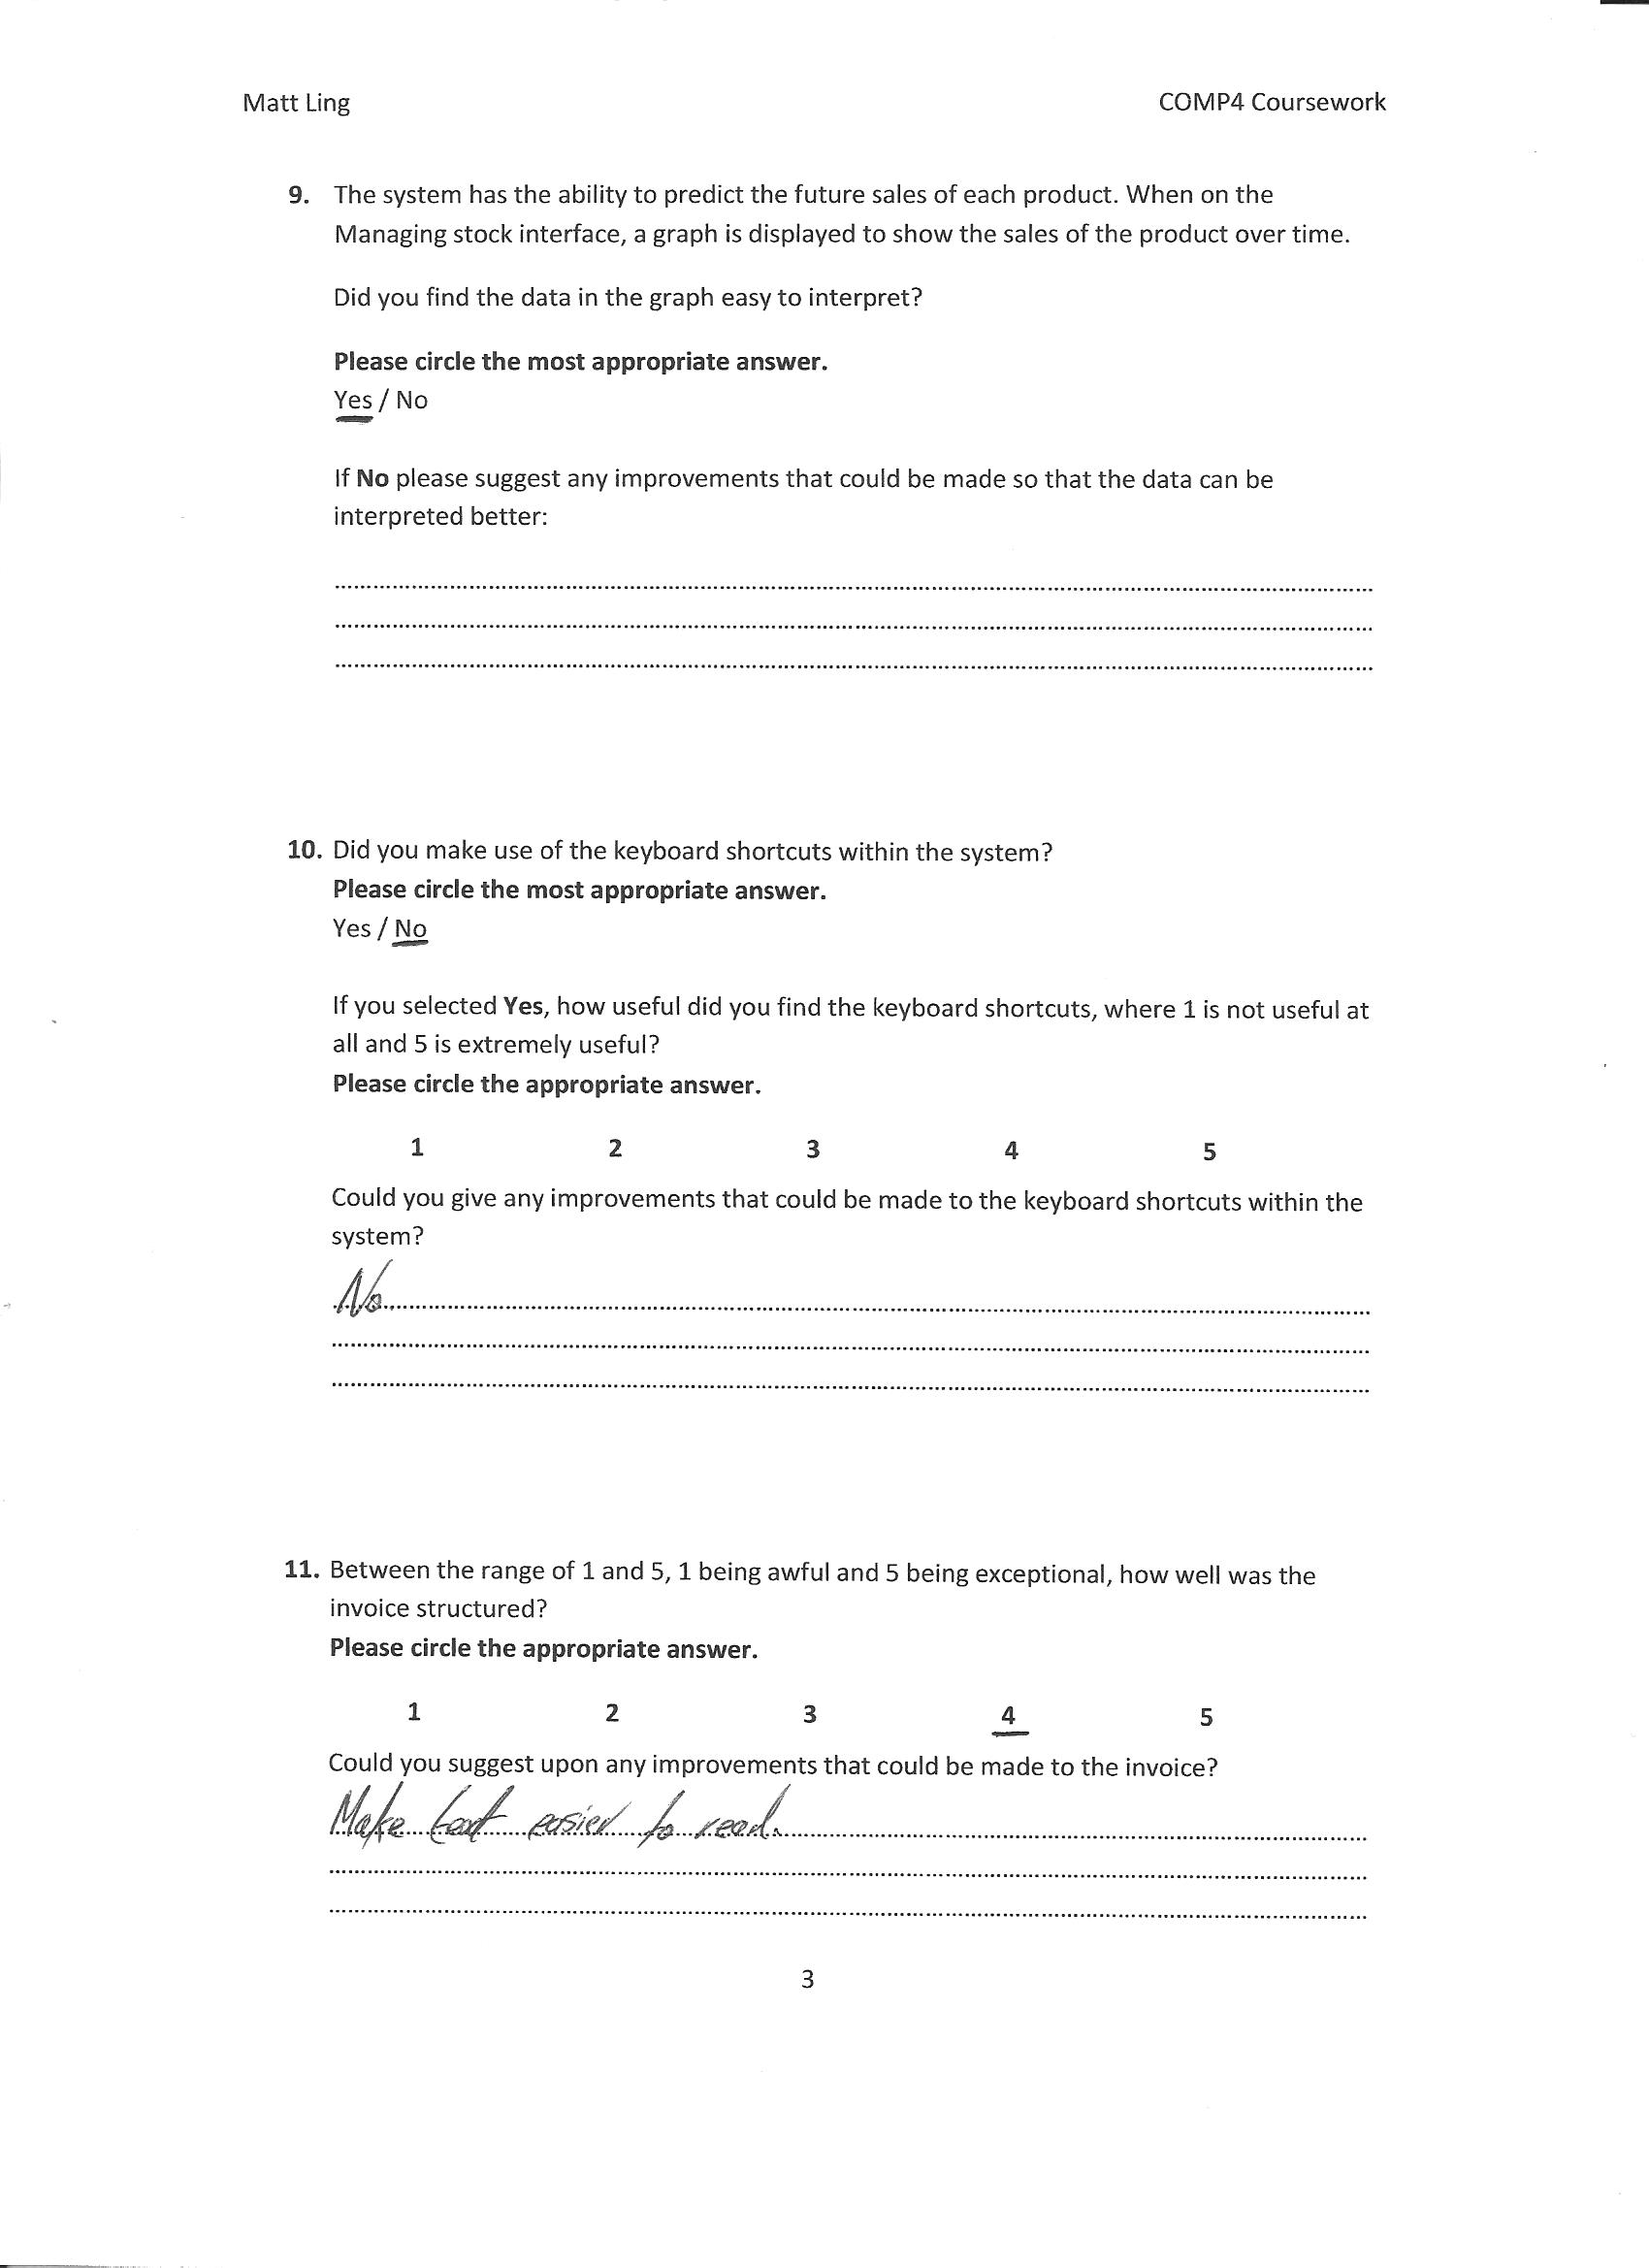
\includepdf{./EvaluationImages/questionaire-3-page-3.jpg}
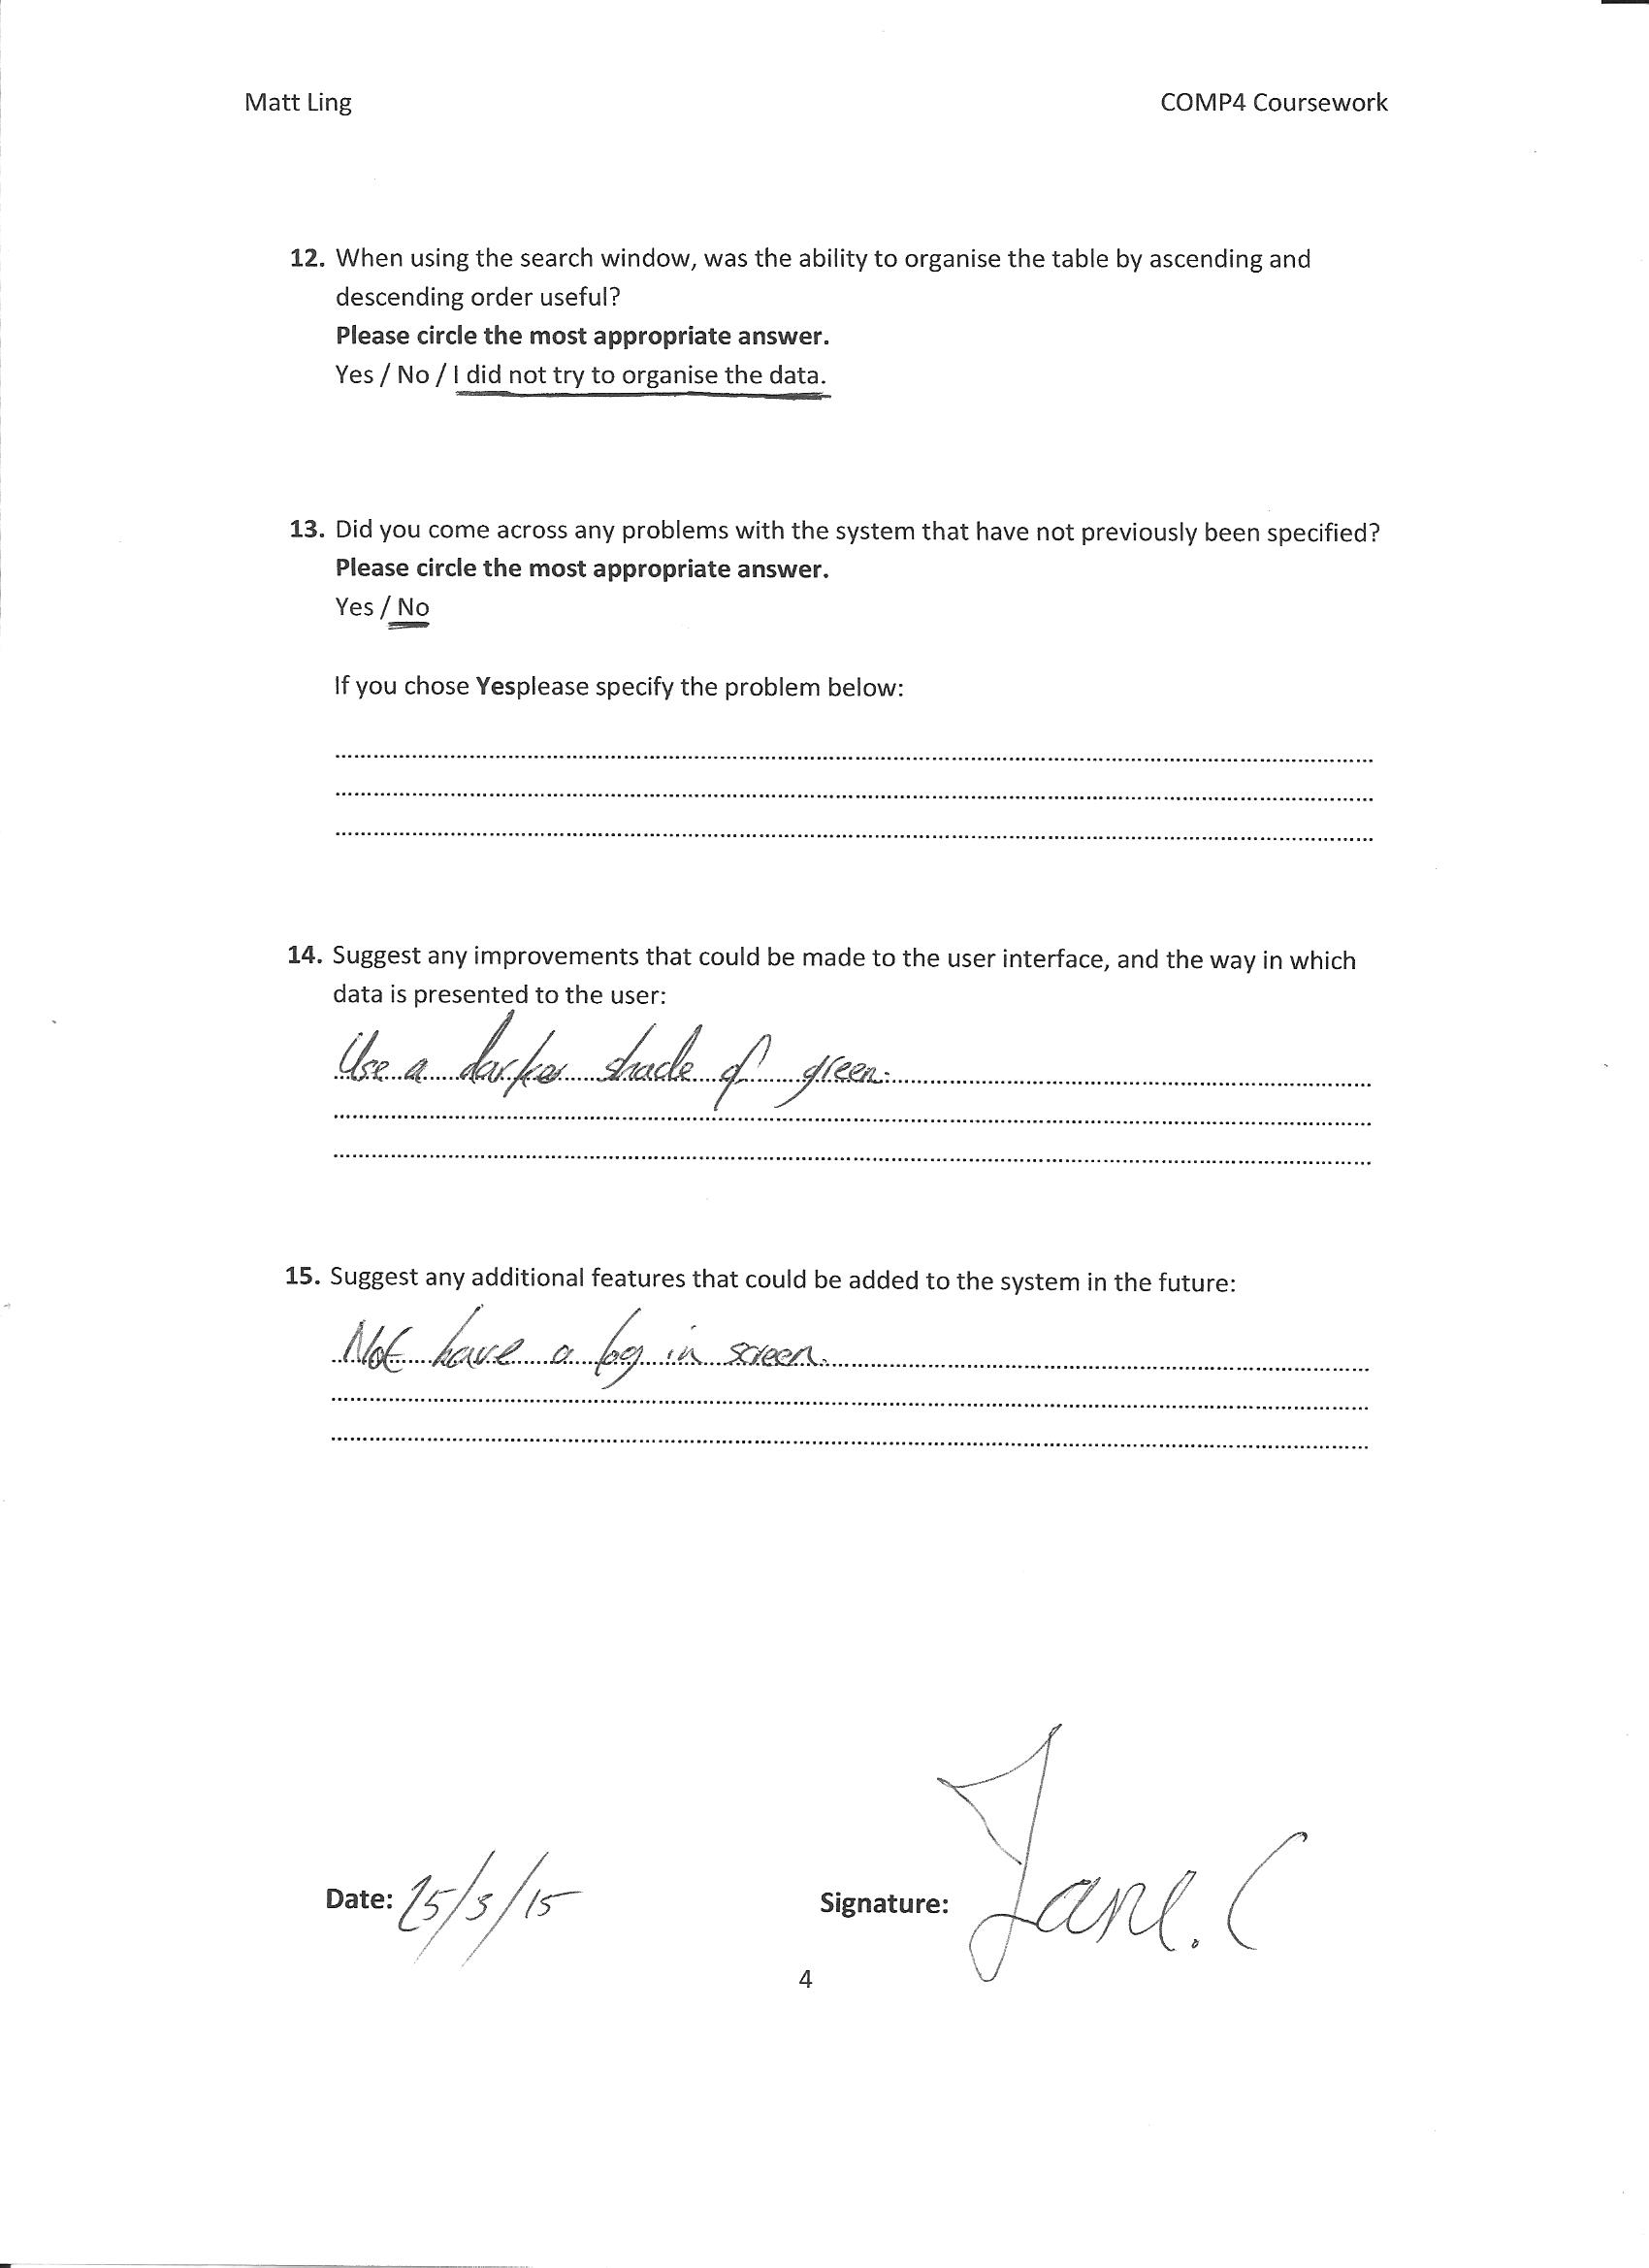
\includepdf{./EvaluationImages/questionaire-3-page-4.jpg}

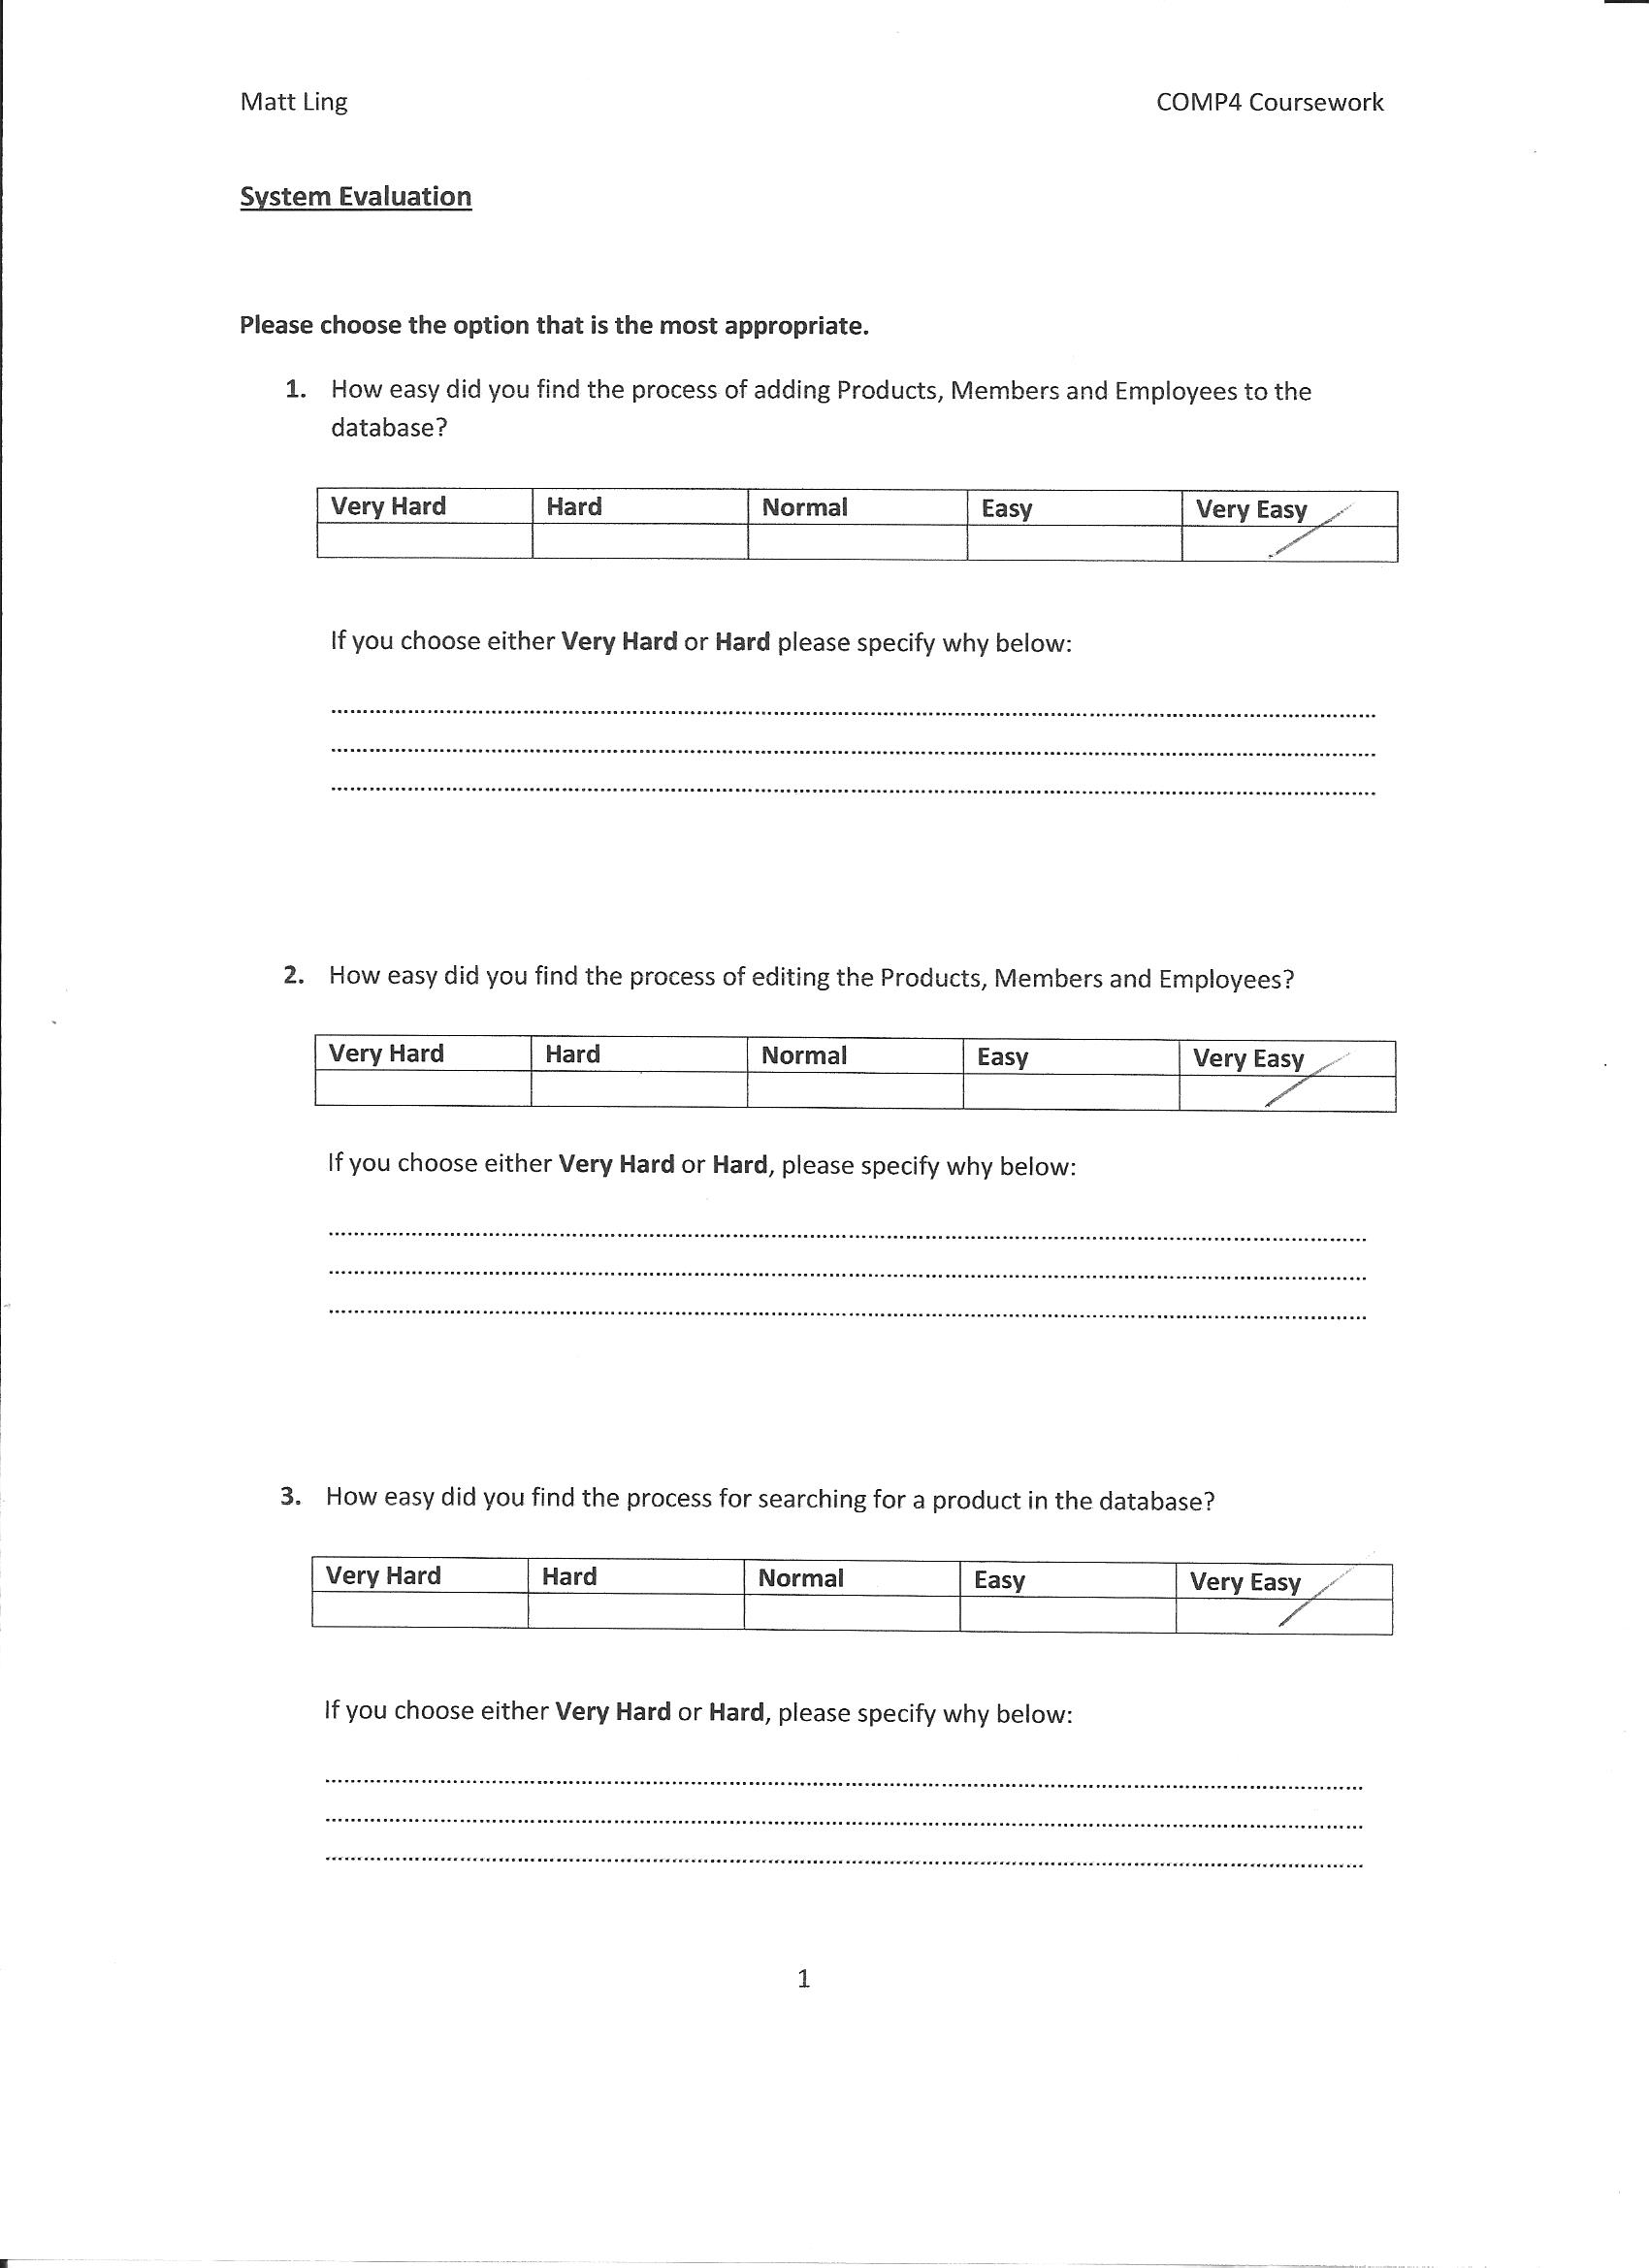
\includepdf{./EvaluationImages/questionaire-4-page-1.jpg}
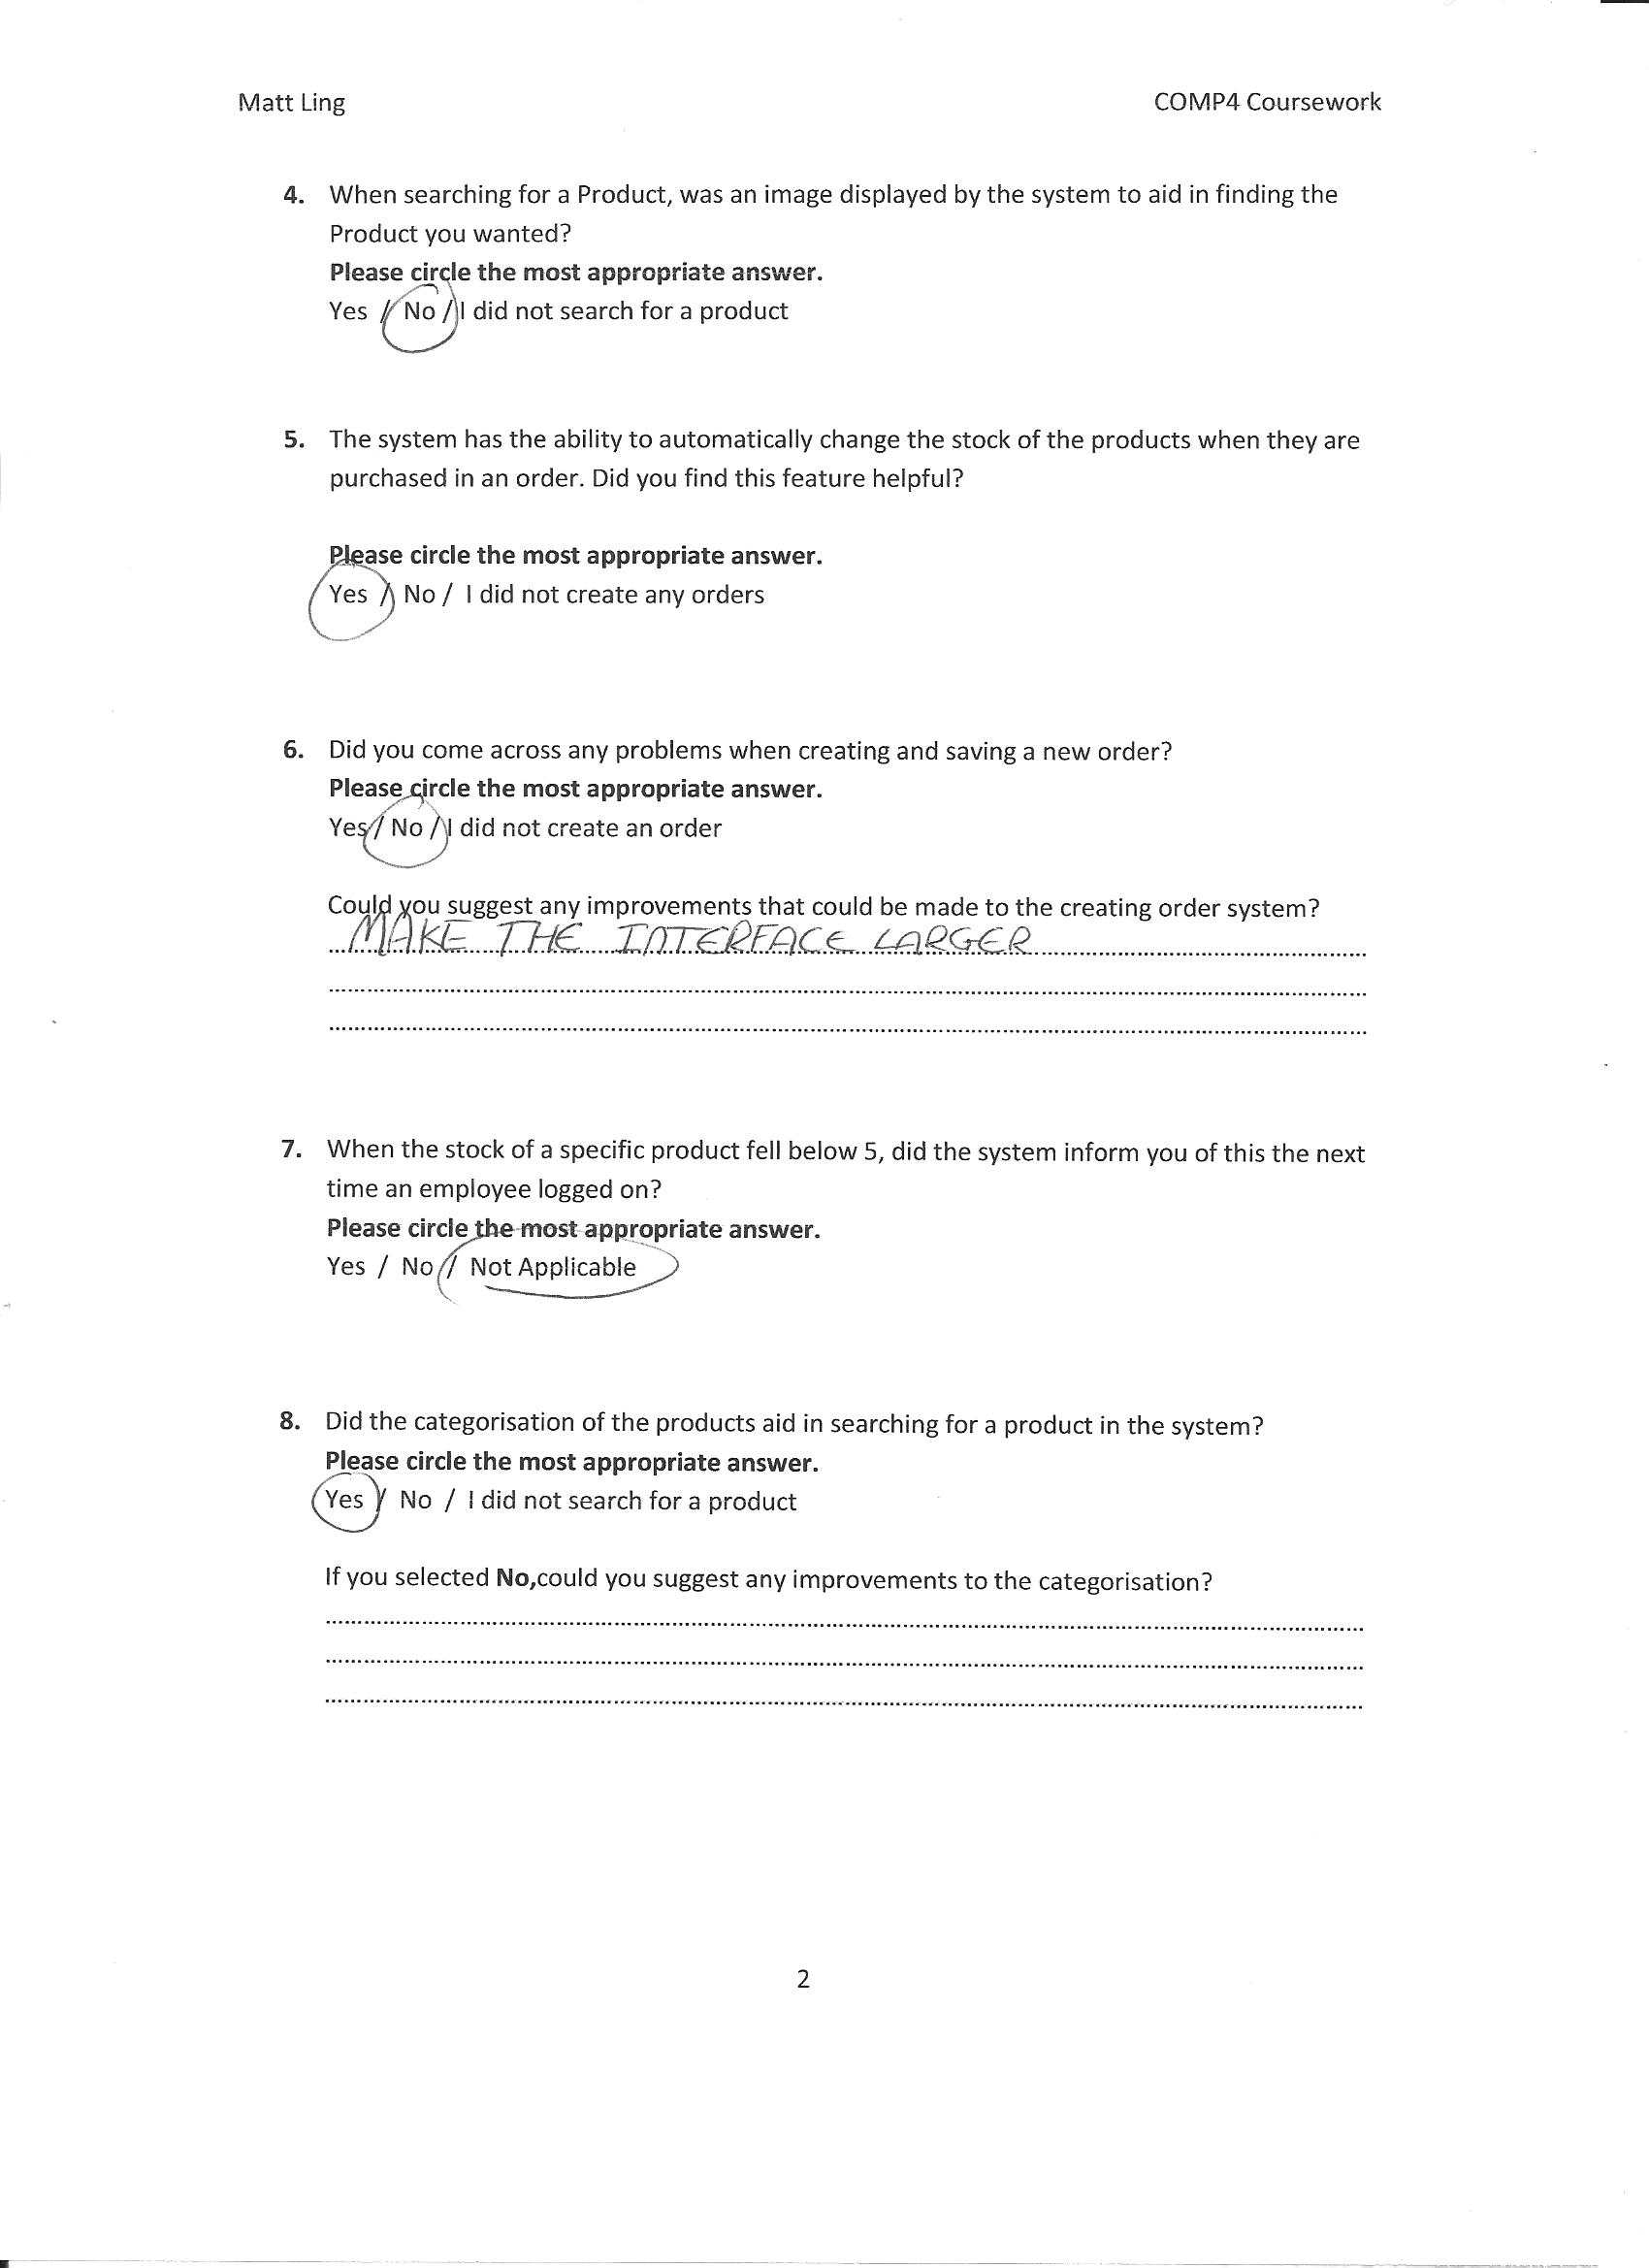
\includepdf{./EvaluationImages/questionaire-4-page-2.jpg}
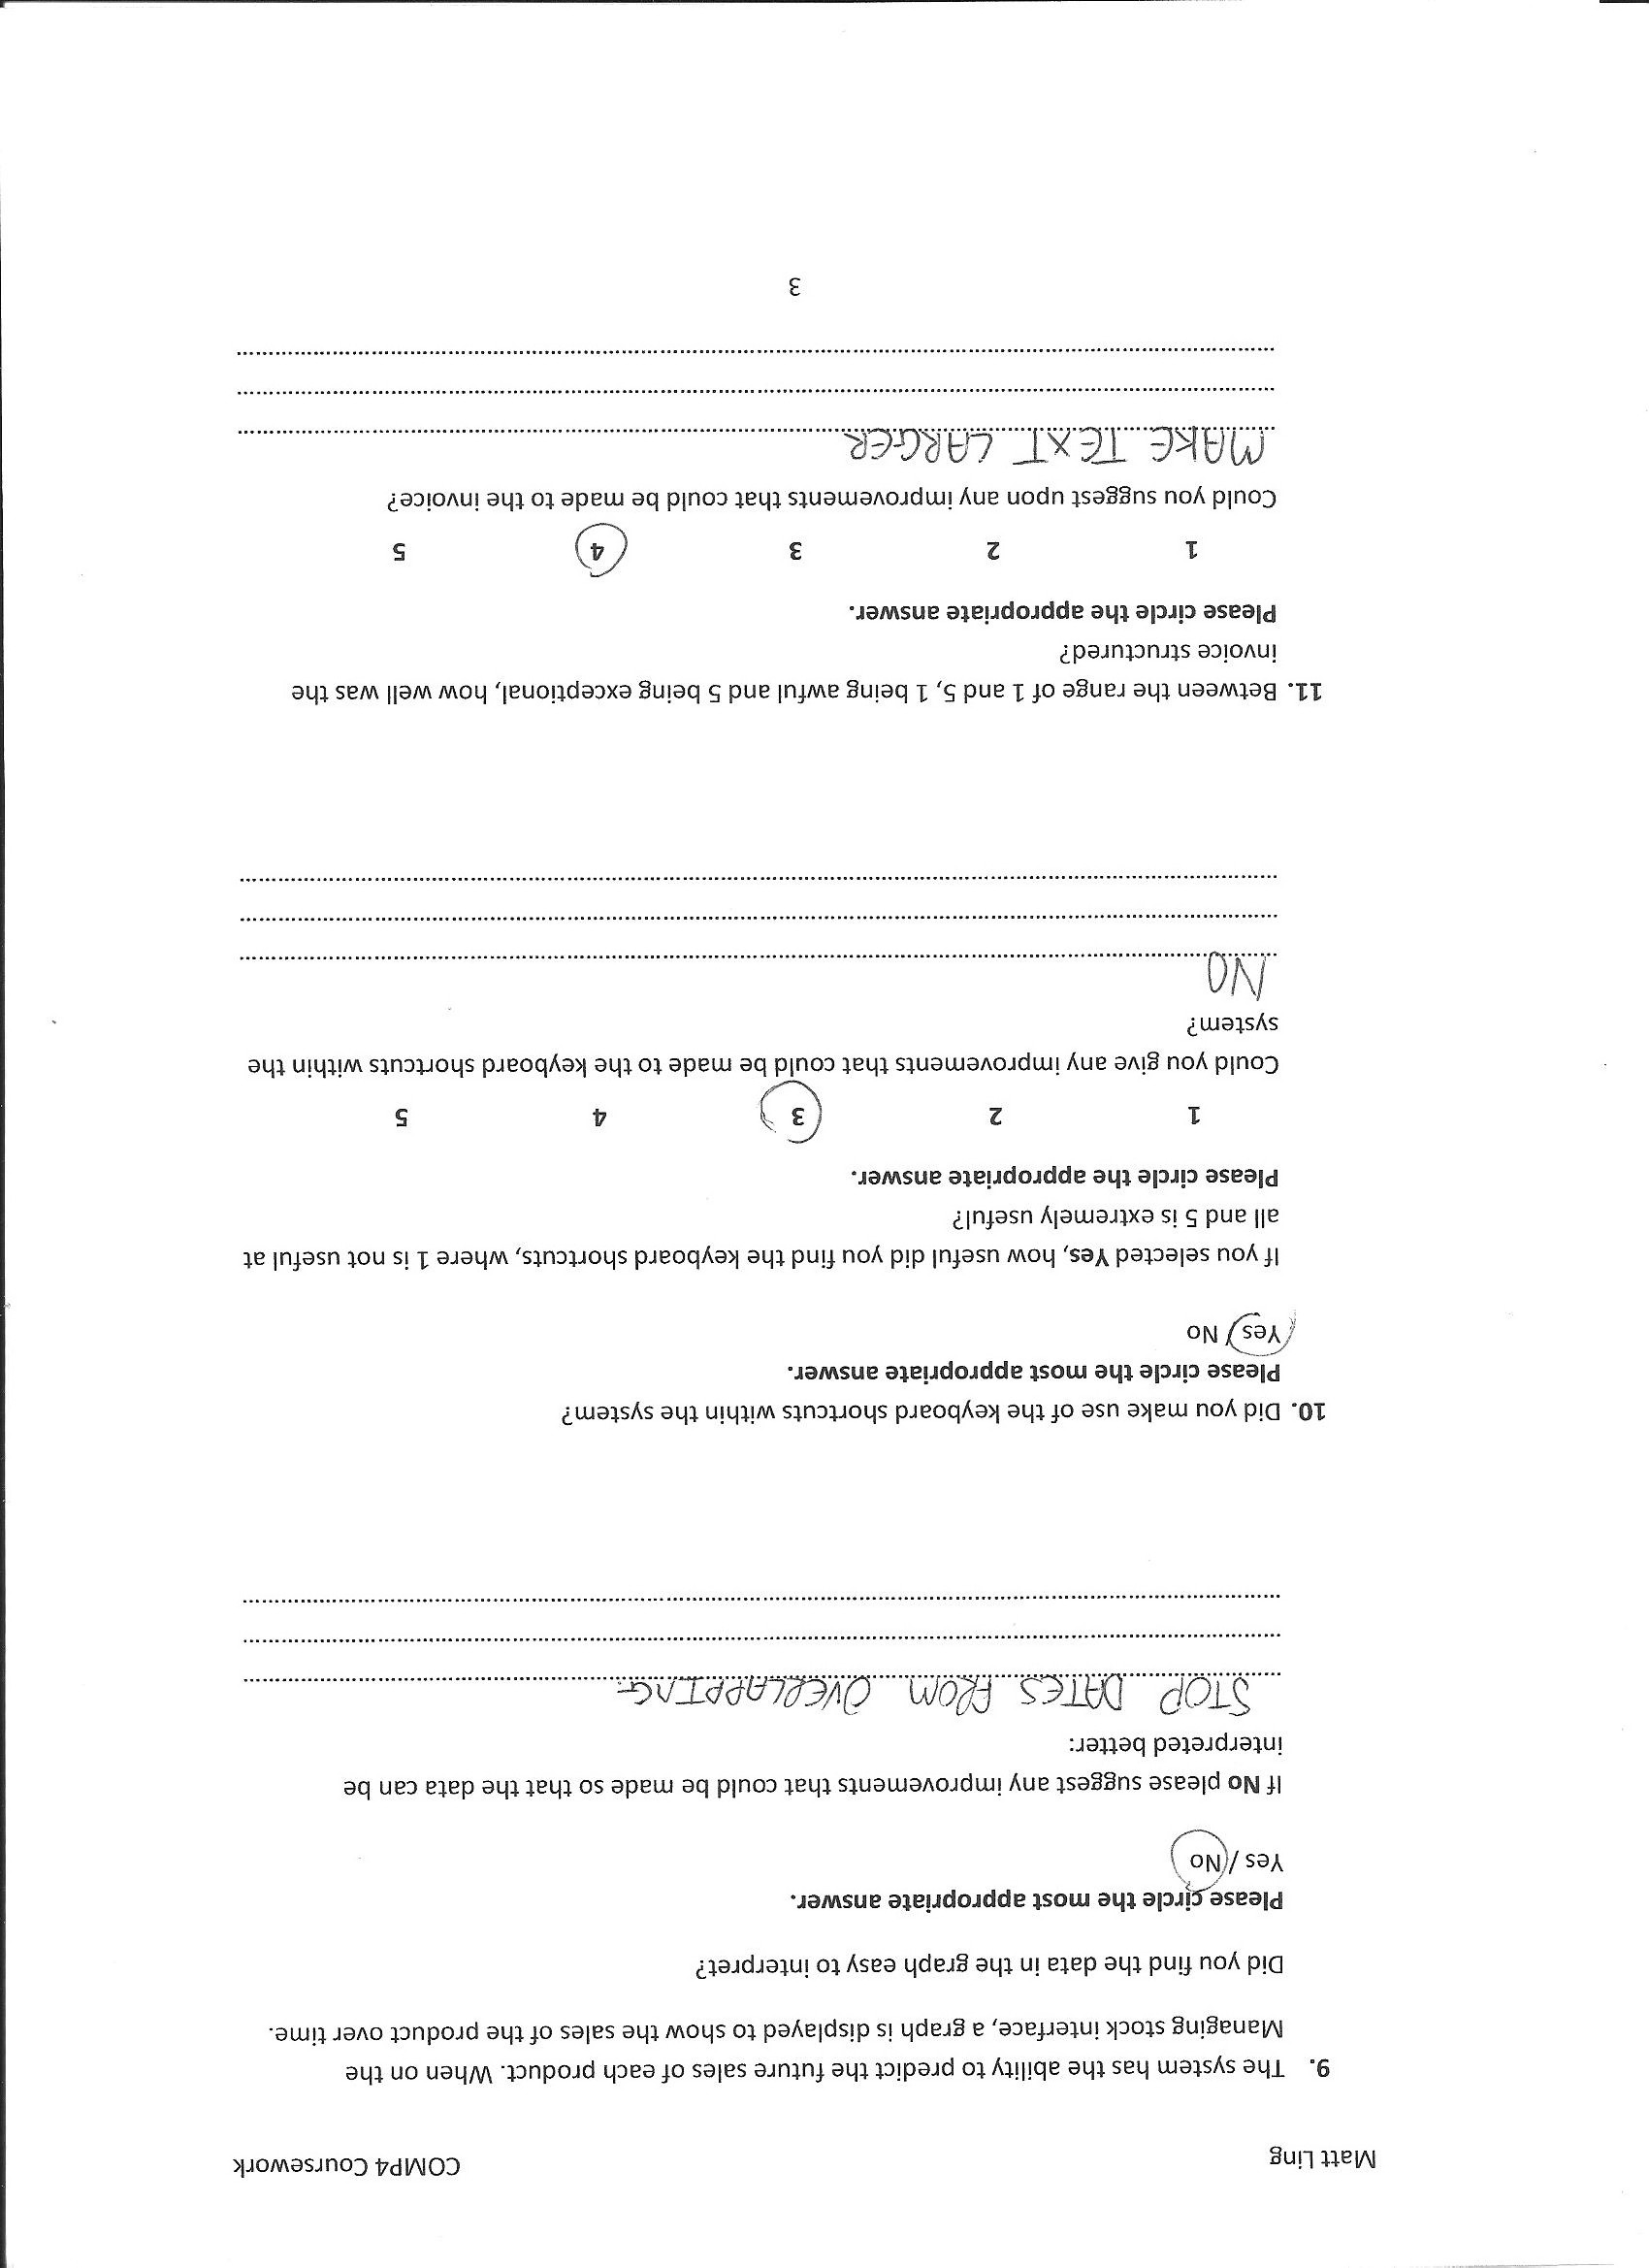
\includepdf{./EvaluationImages/questionaire-4-page-3.jpg}
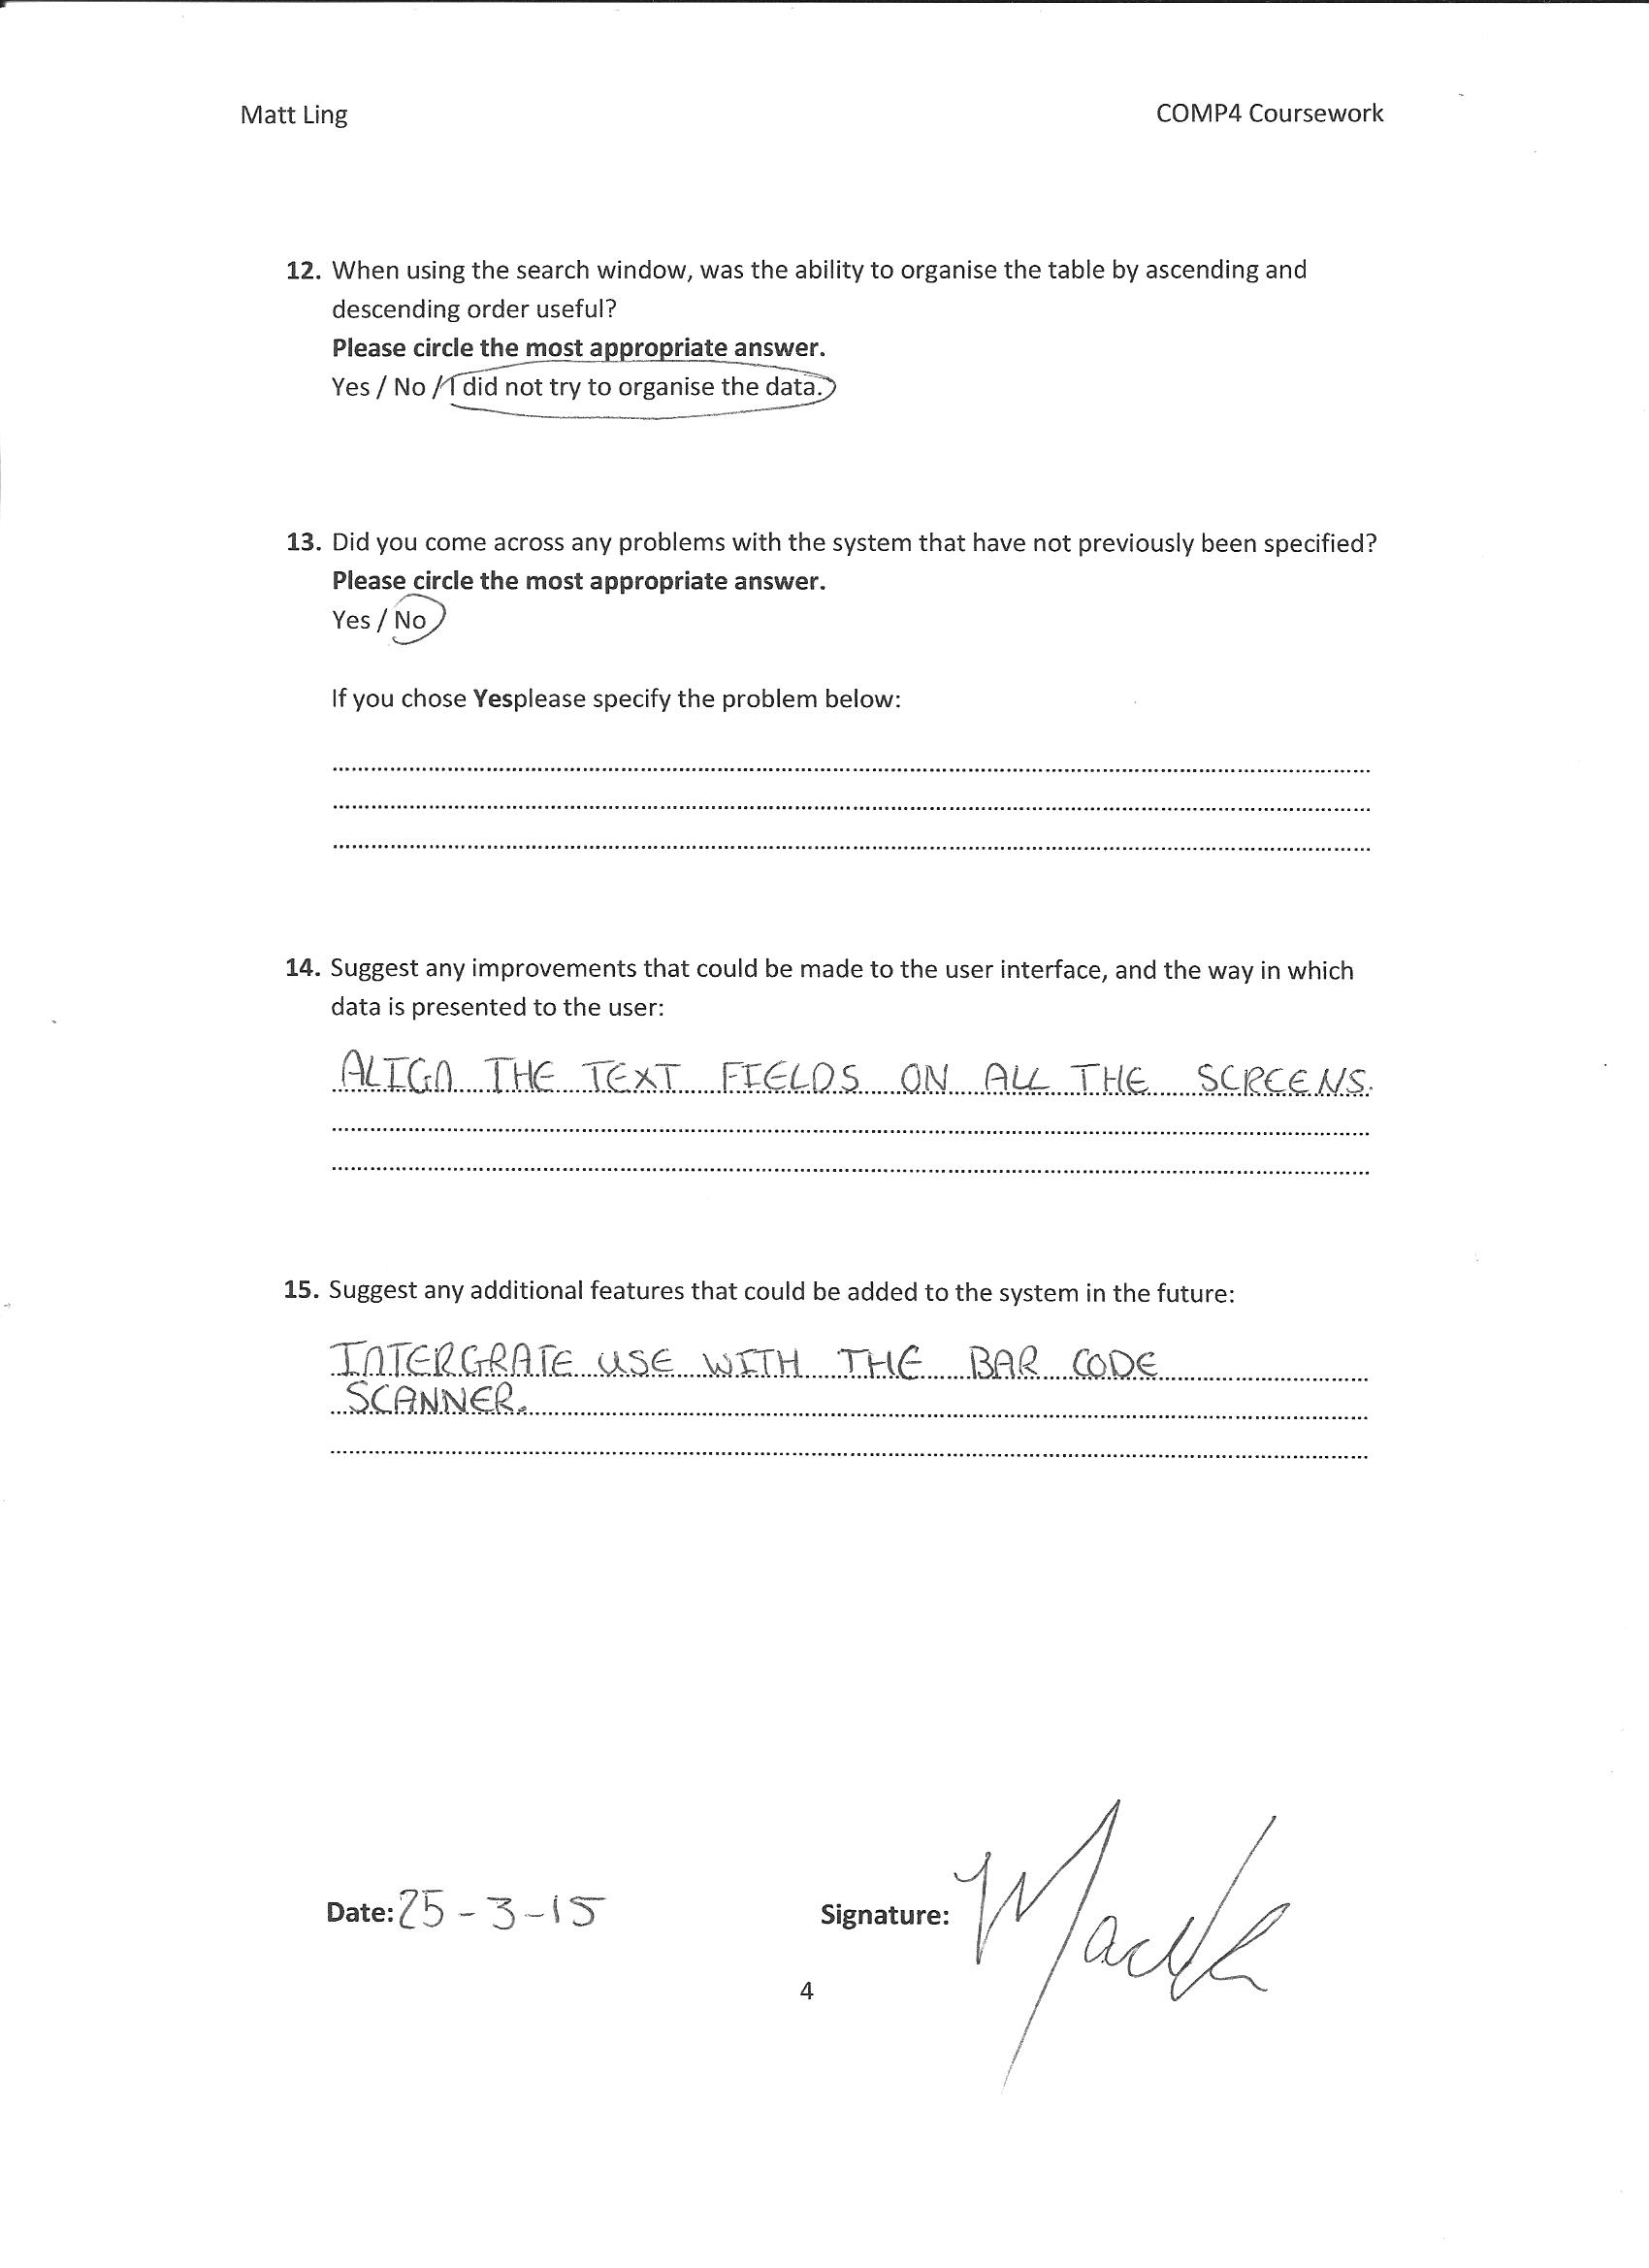
\includepdf{./EvaluationImages/questionaire-4-page-4.jpg}

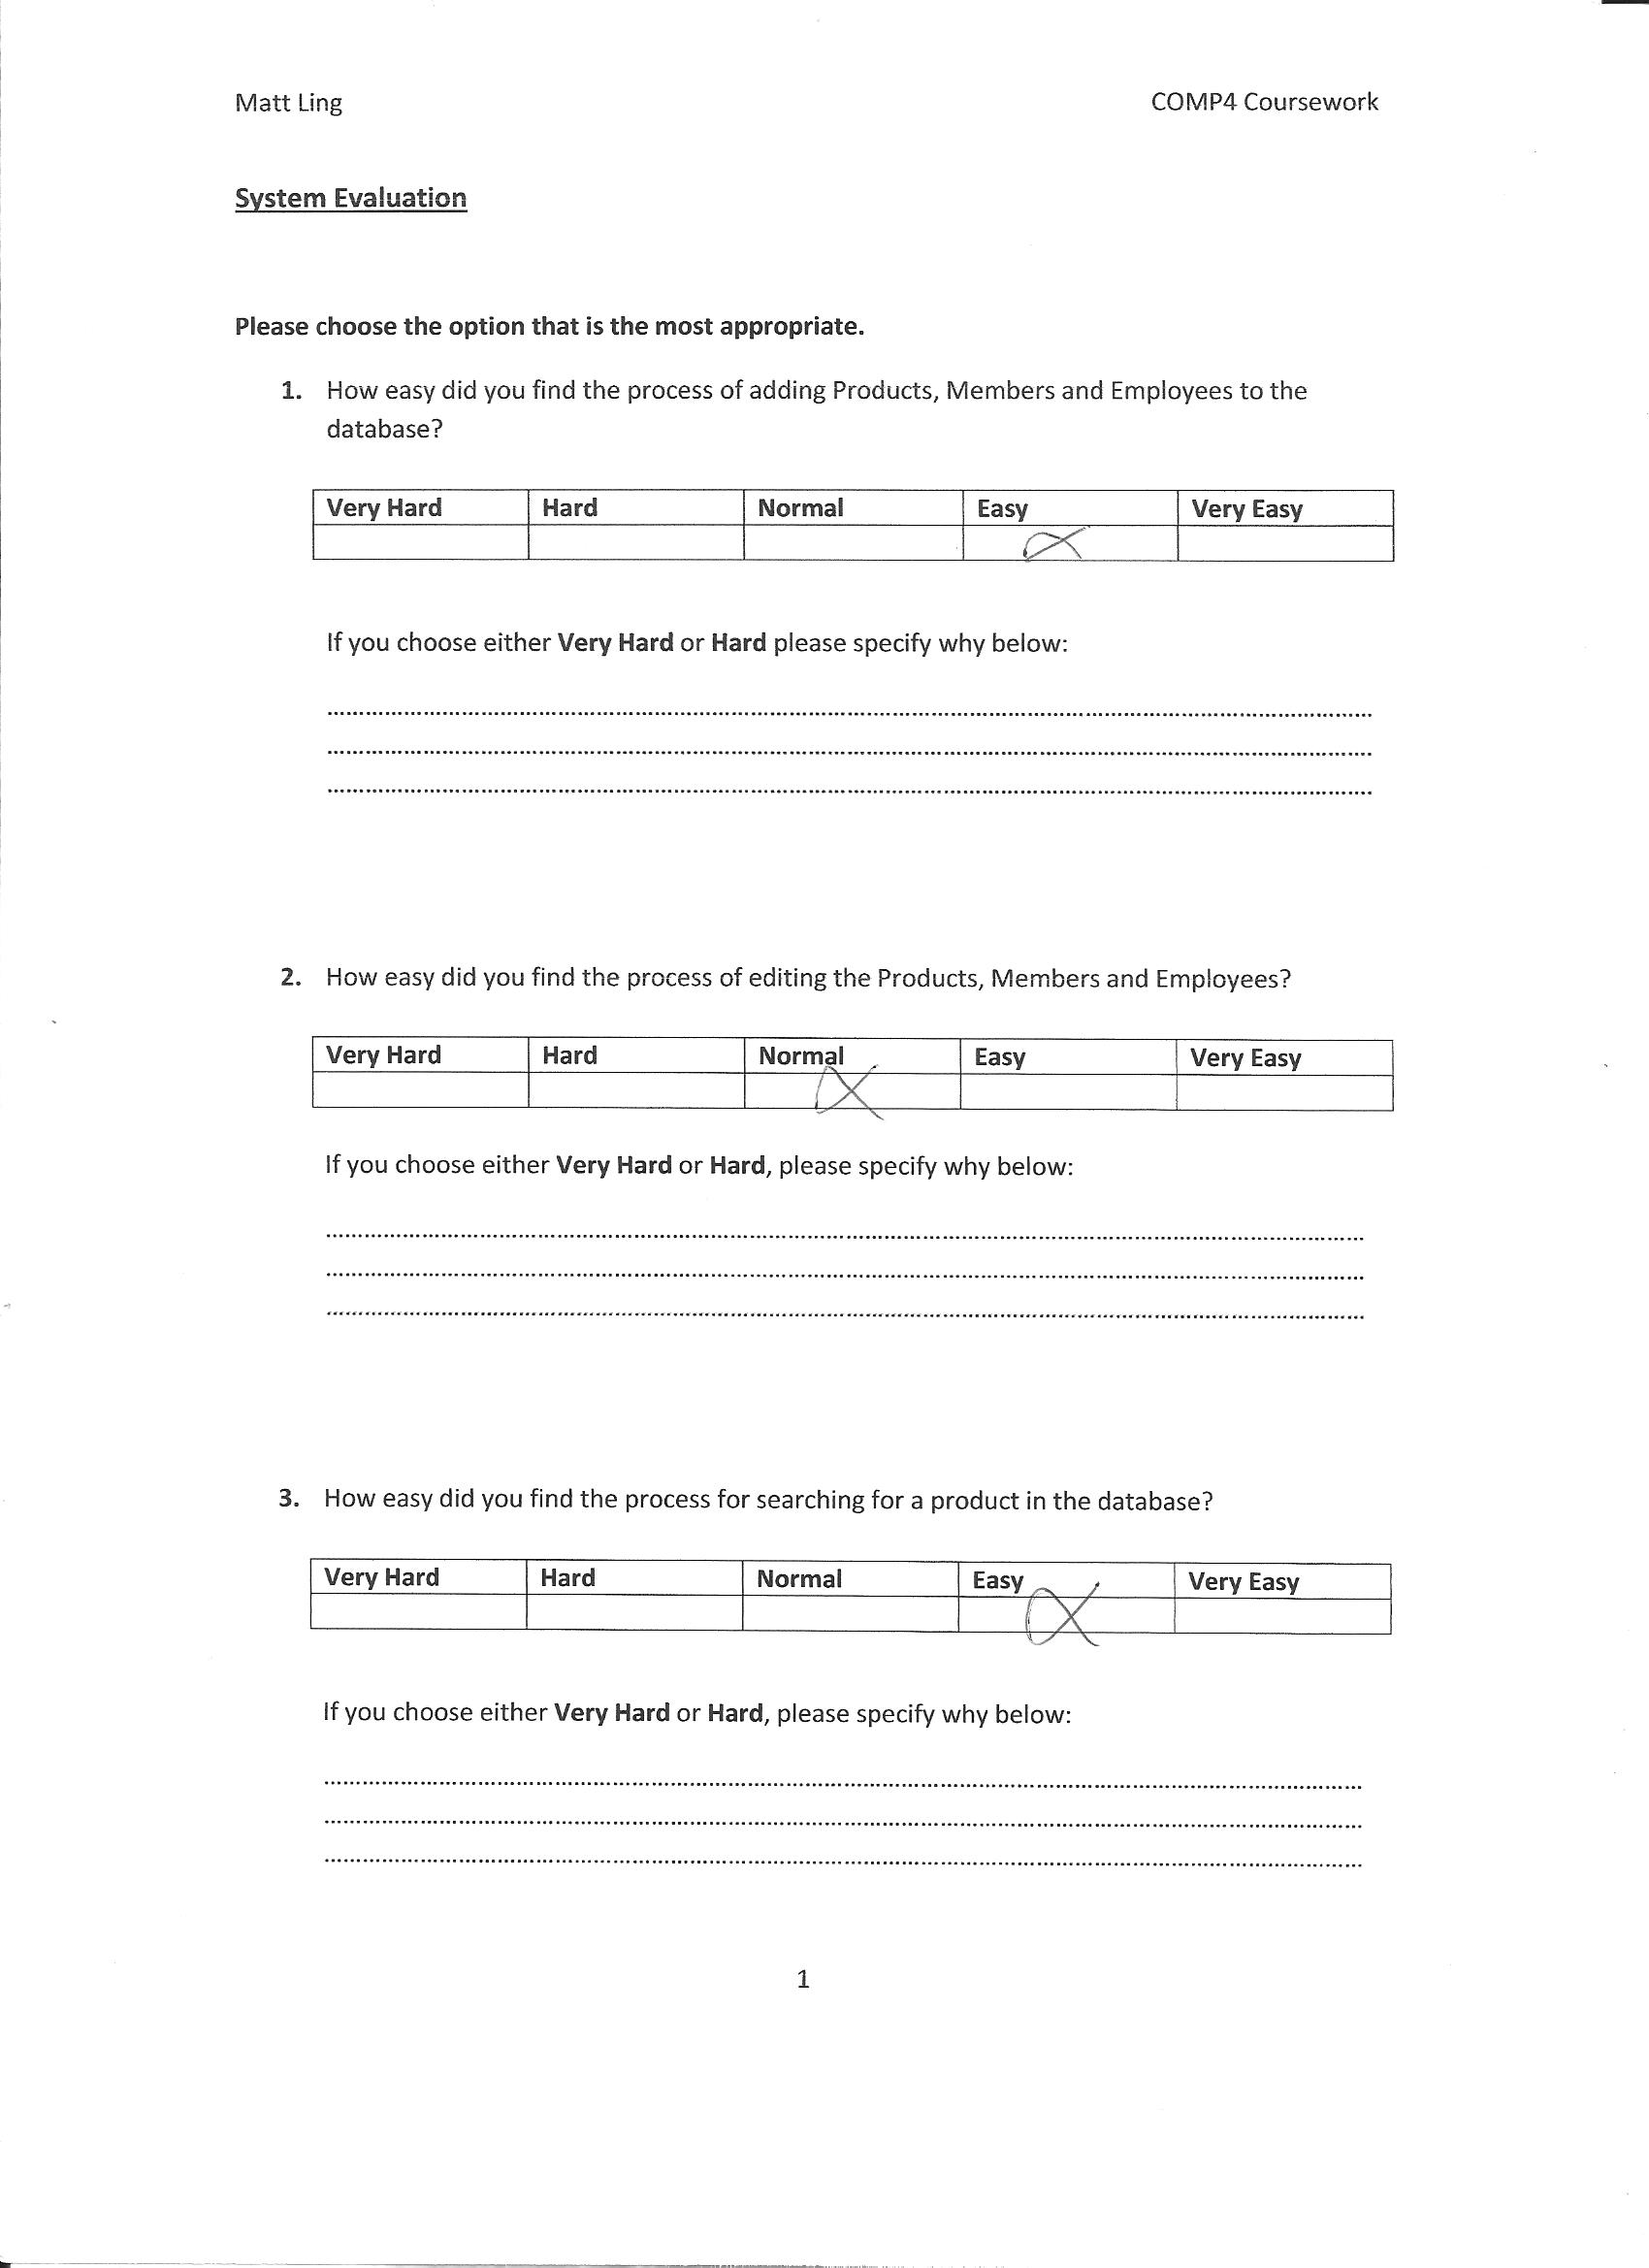
\includepdf{./EvaluationImages/questionaire-5-page-1.jpg}
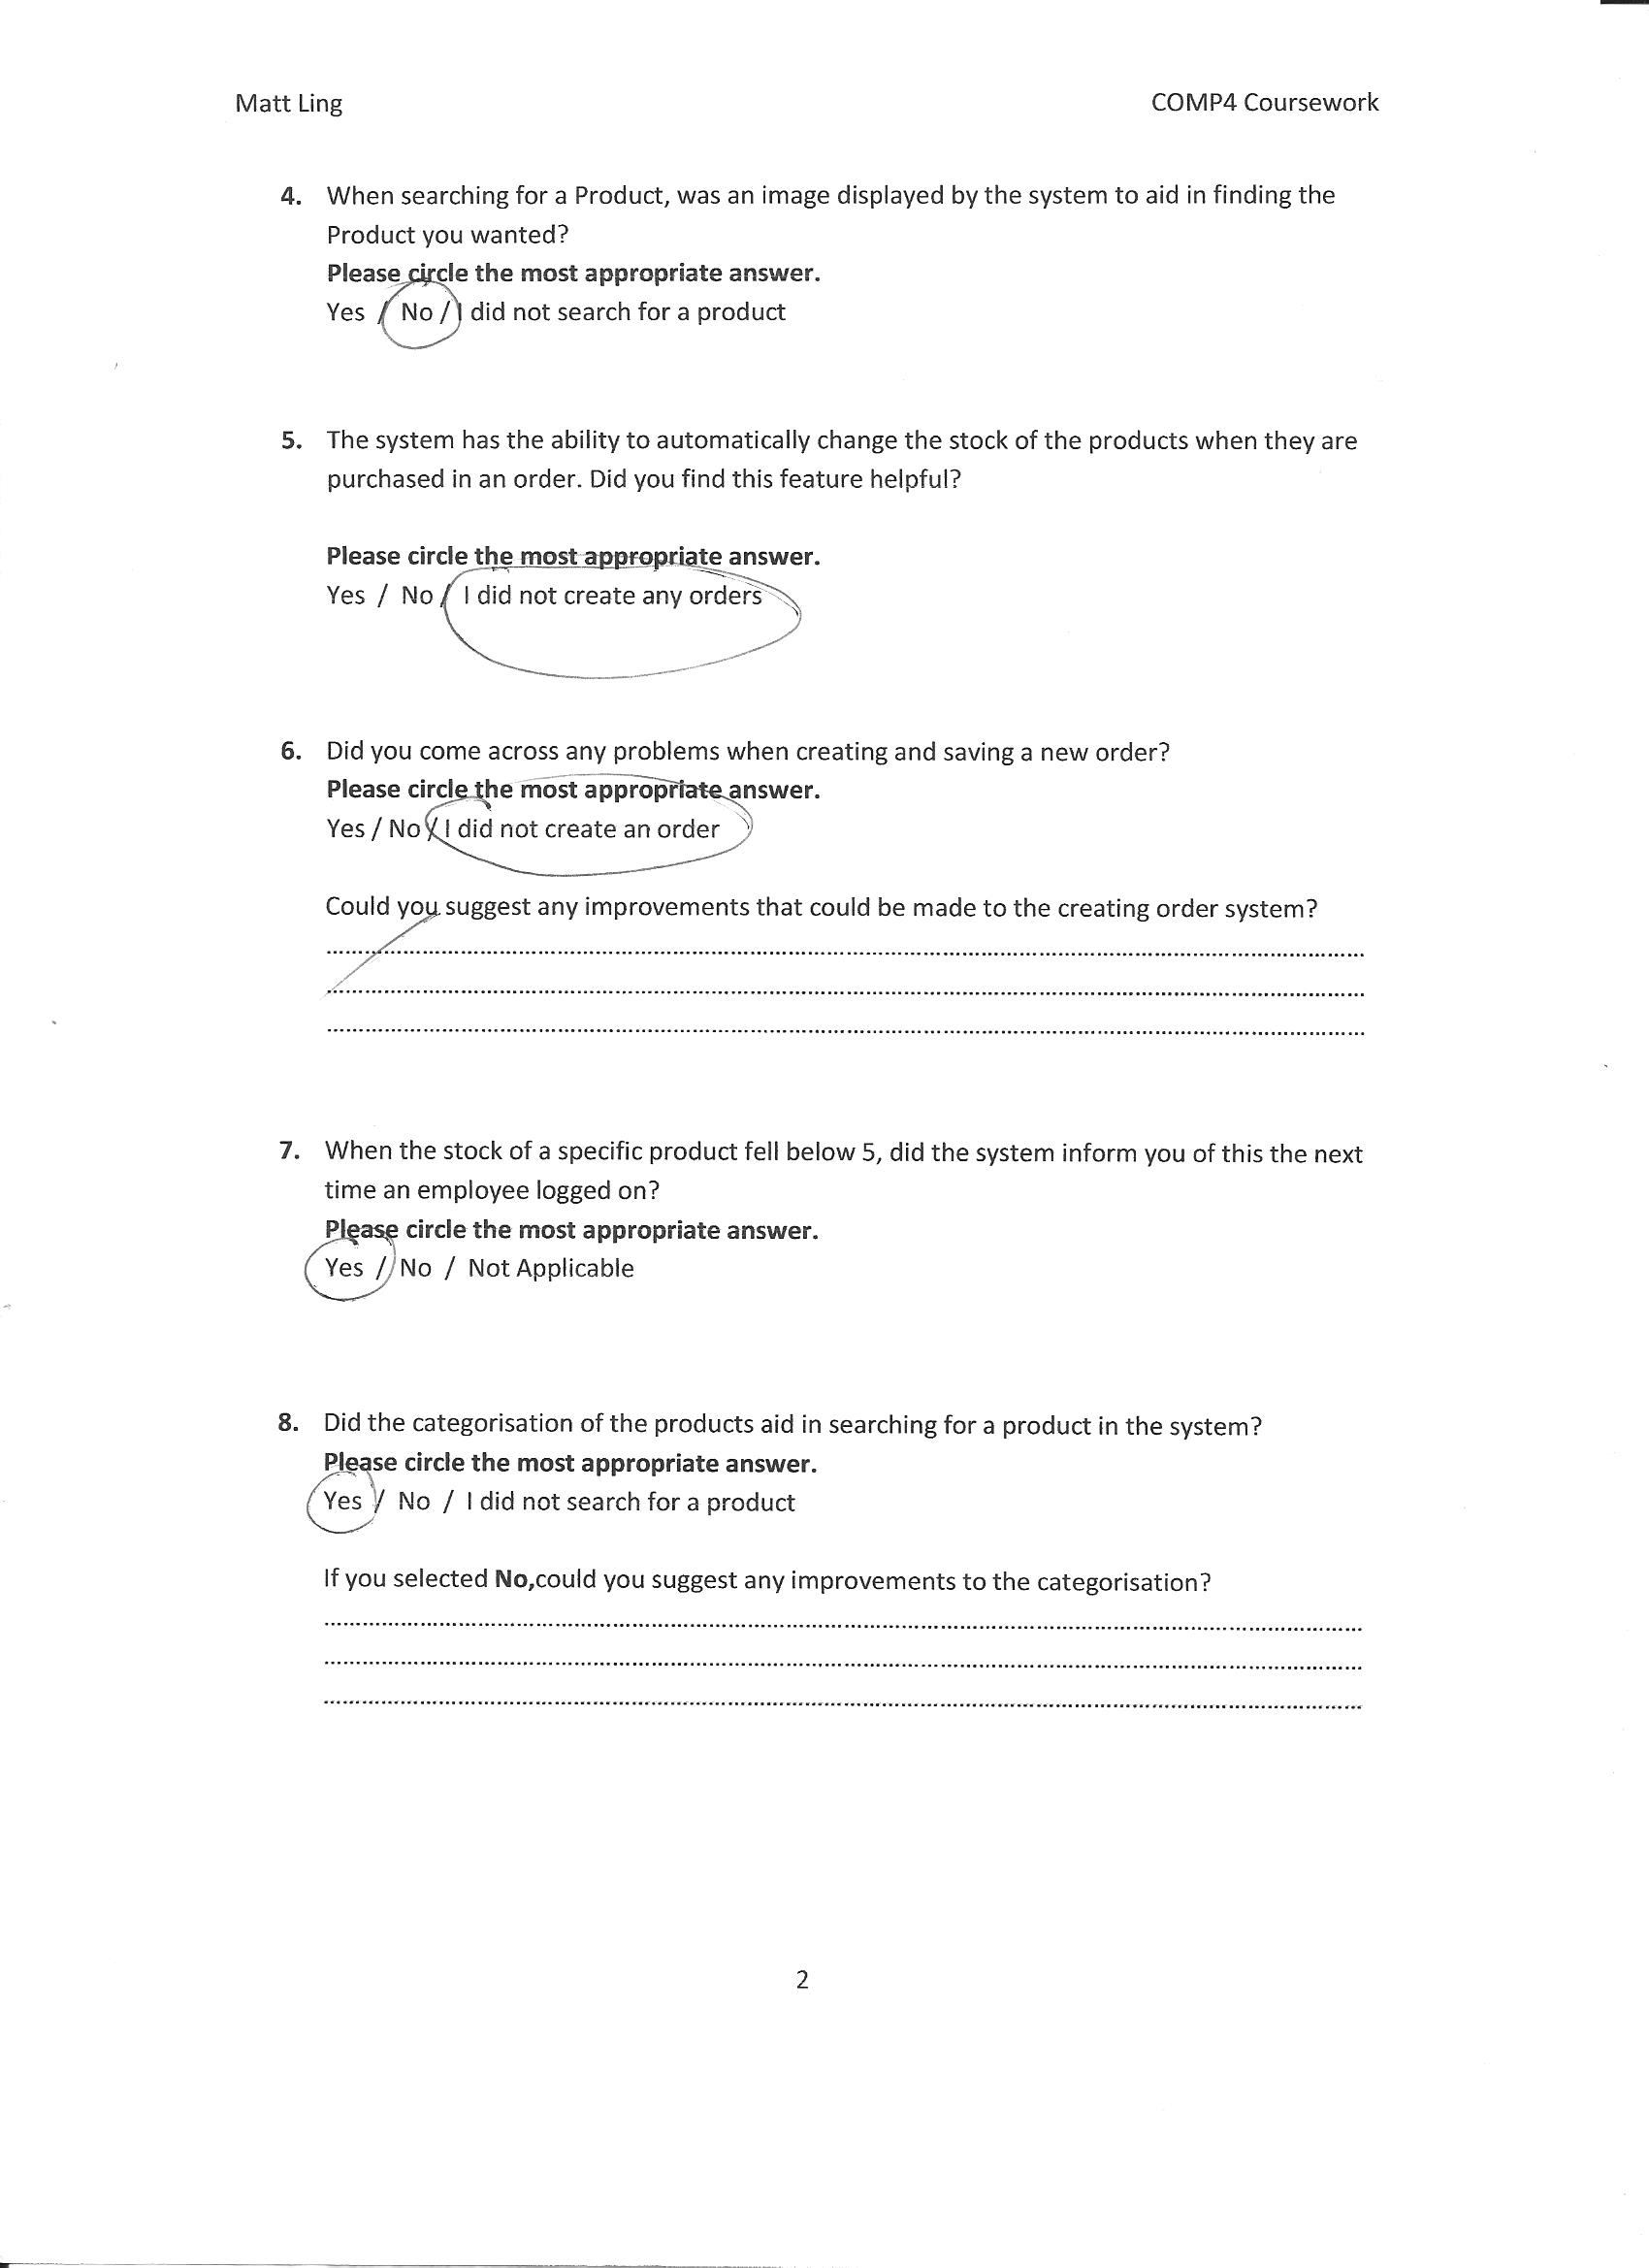
\includepdf{./EvaluationImages/questionaire-5-page-2.jpg}
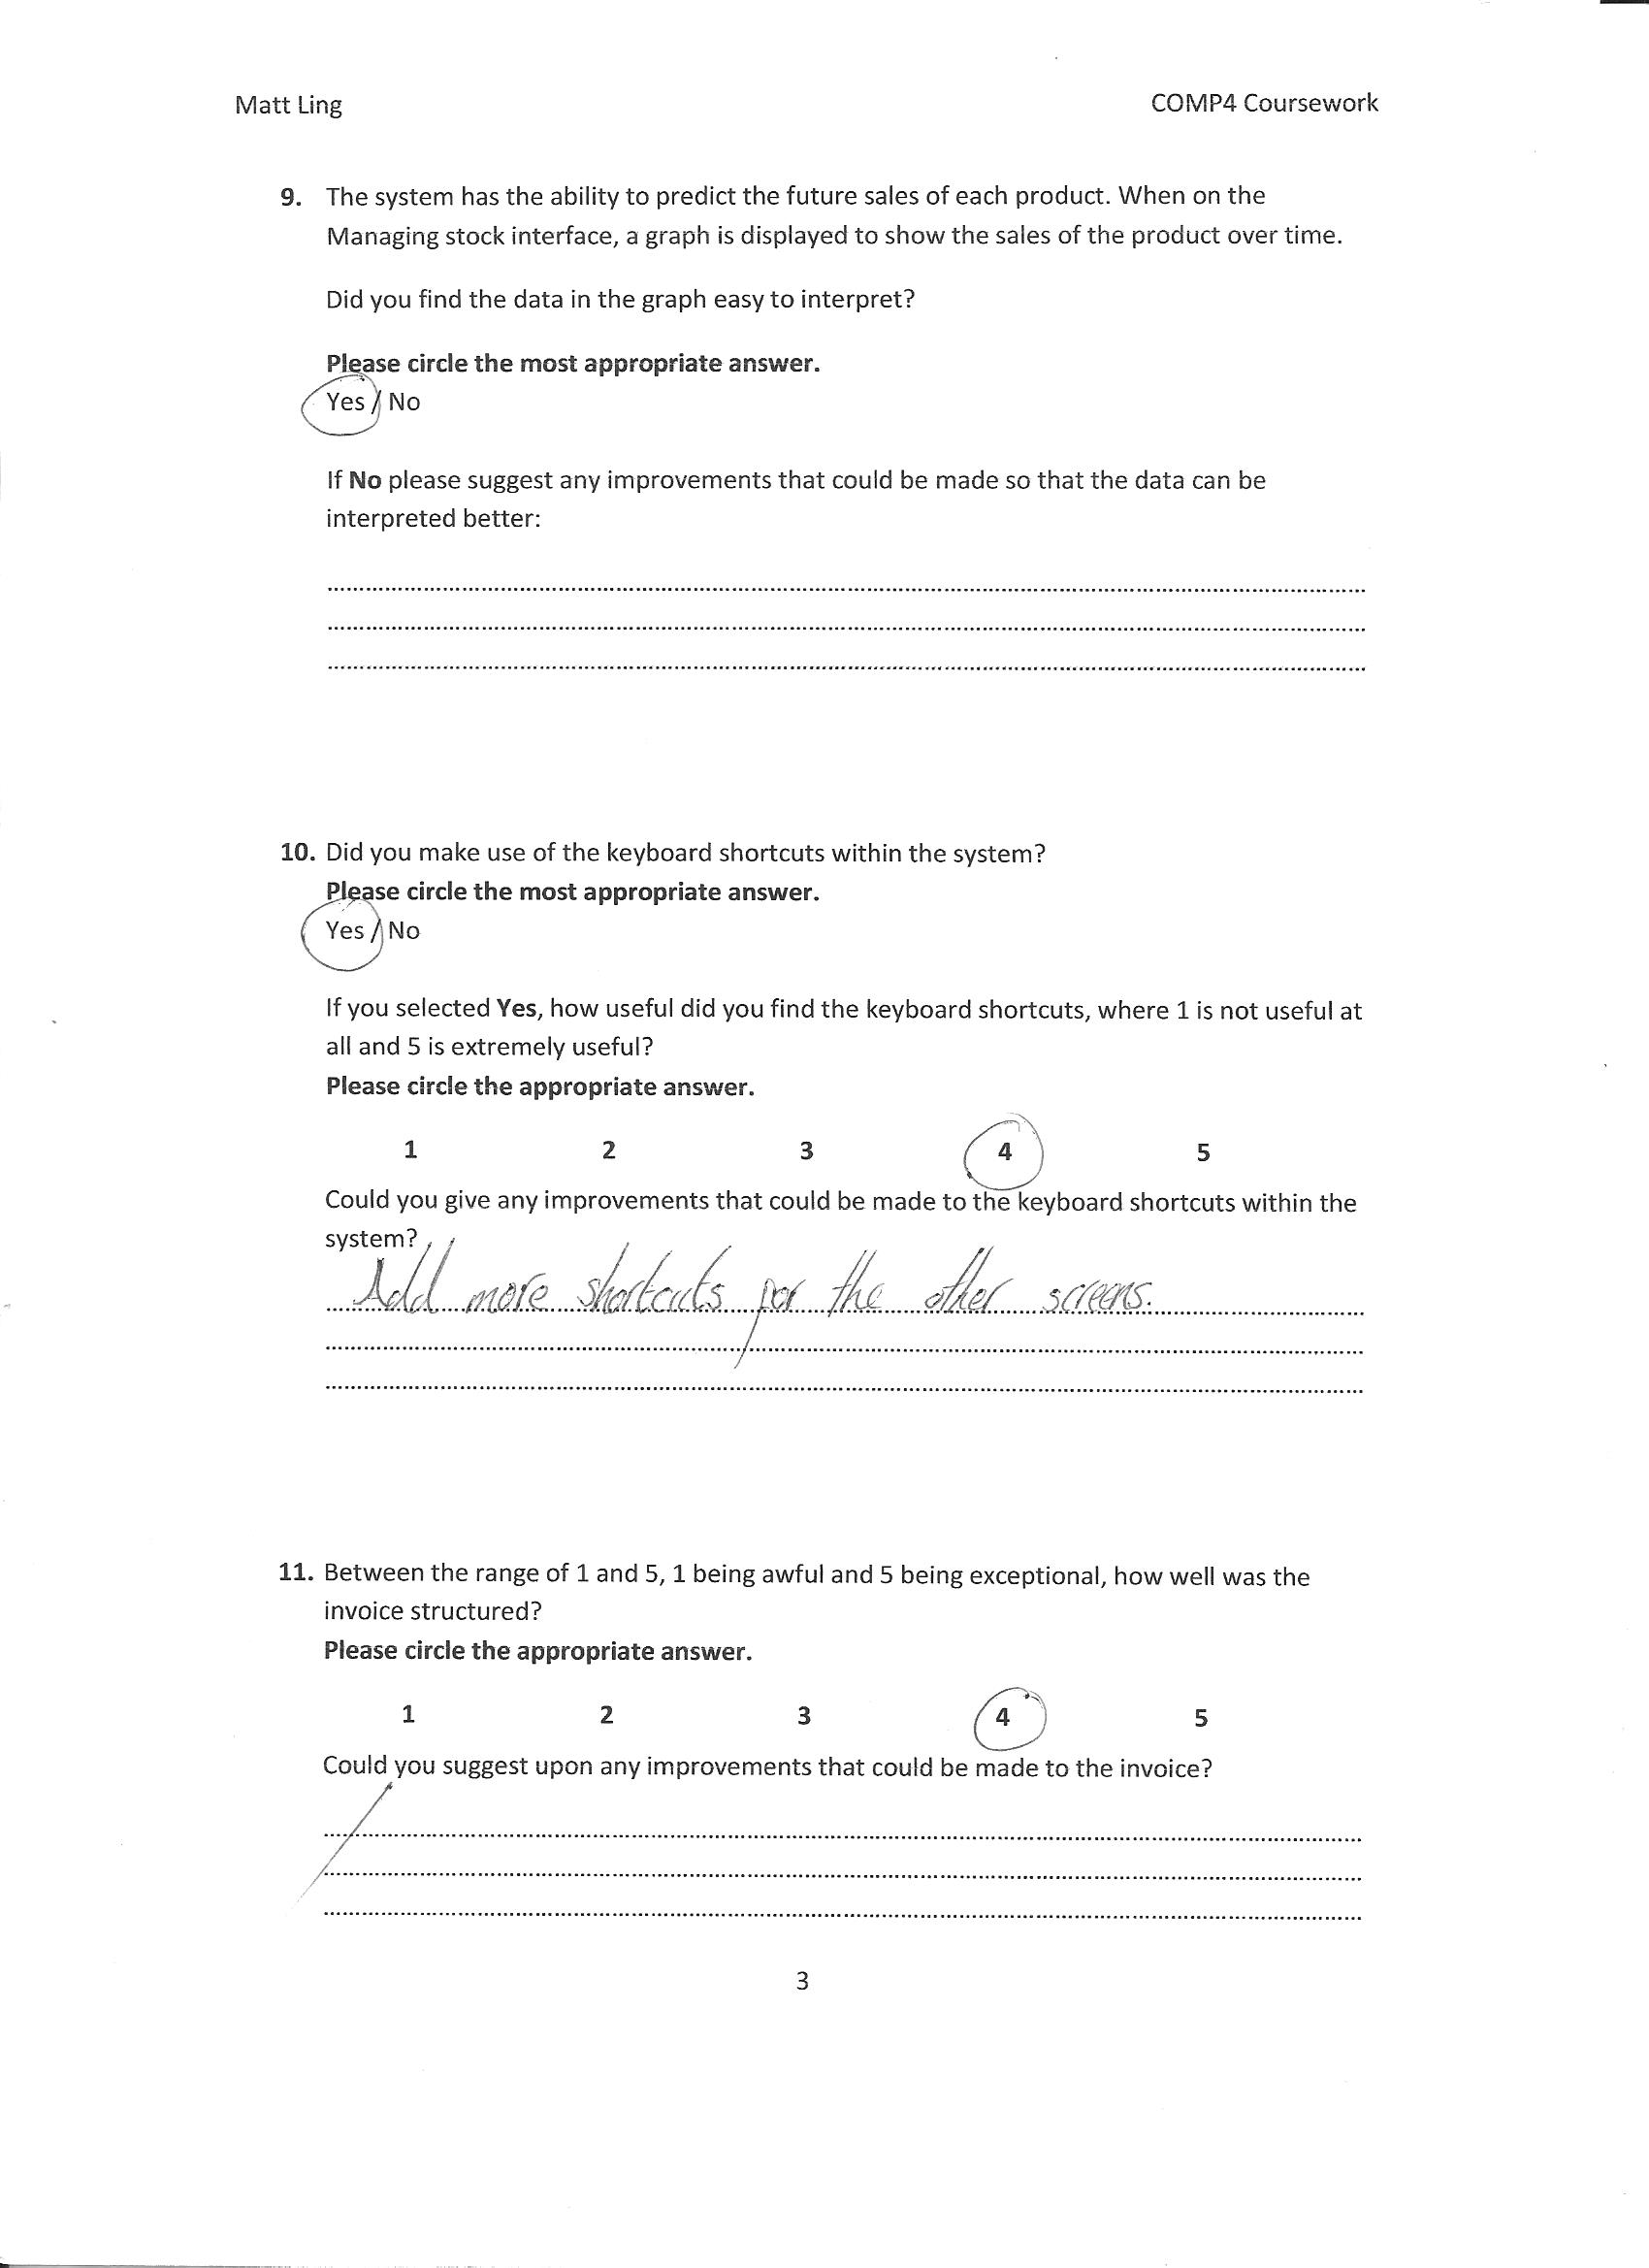
\includepdf{./EvaluationImages/questionaire-5-page-3.jpg}
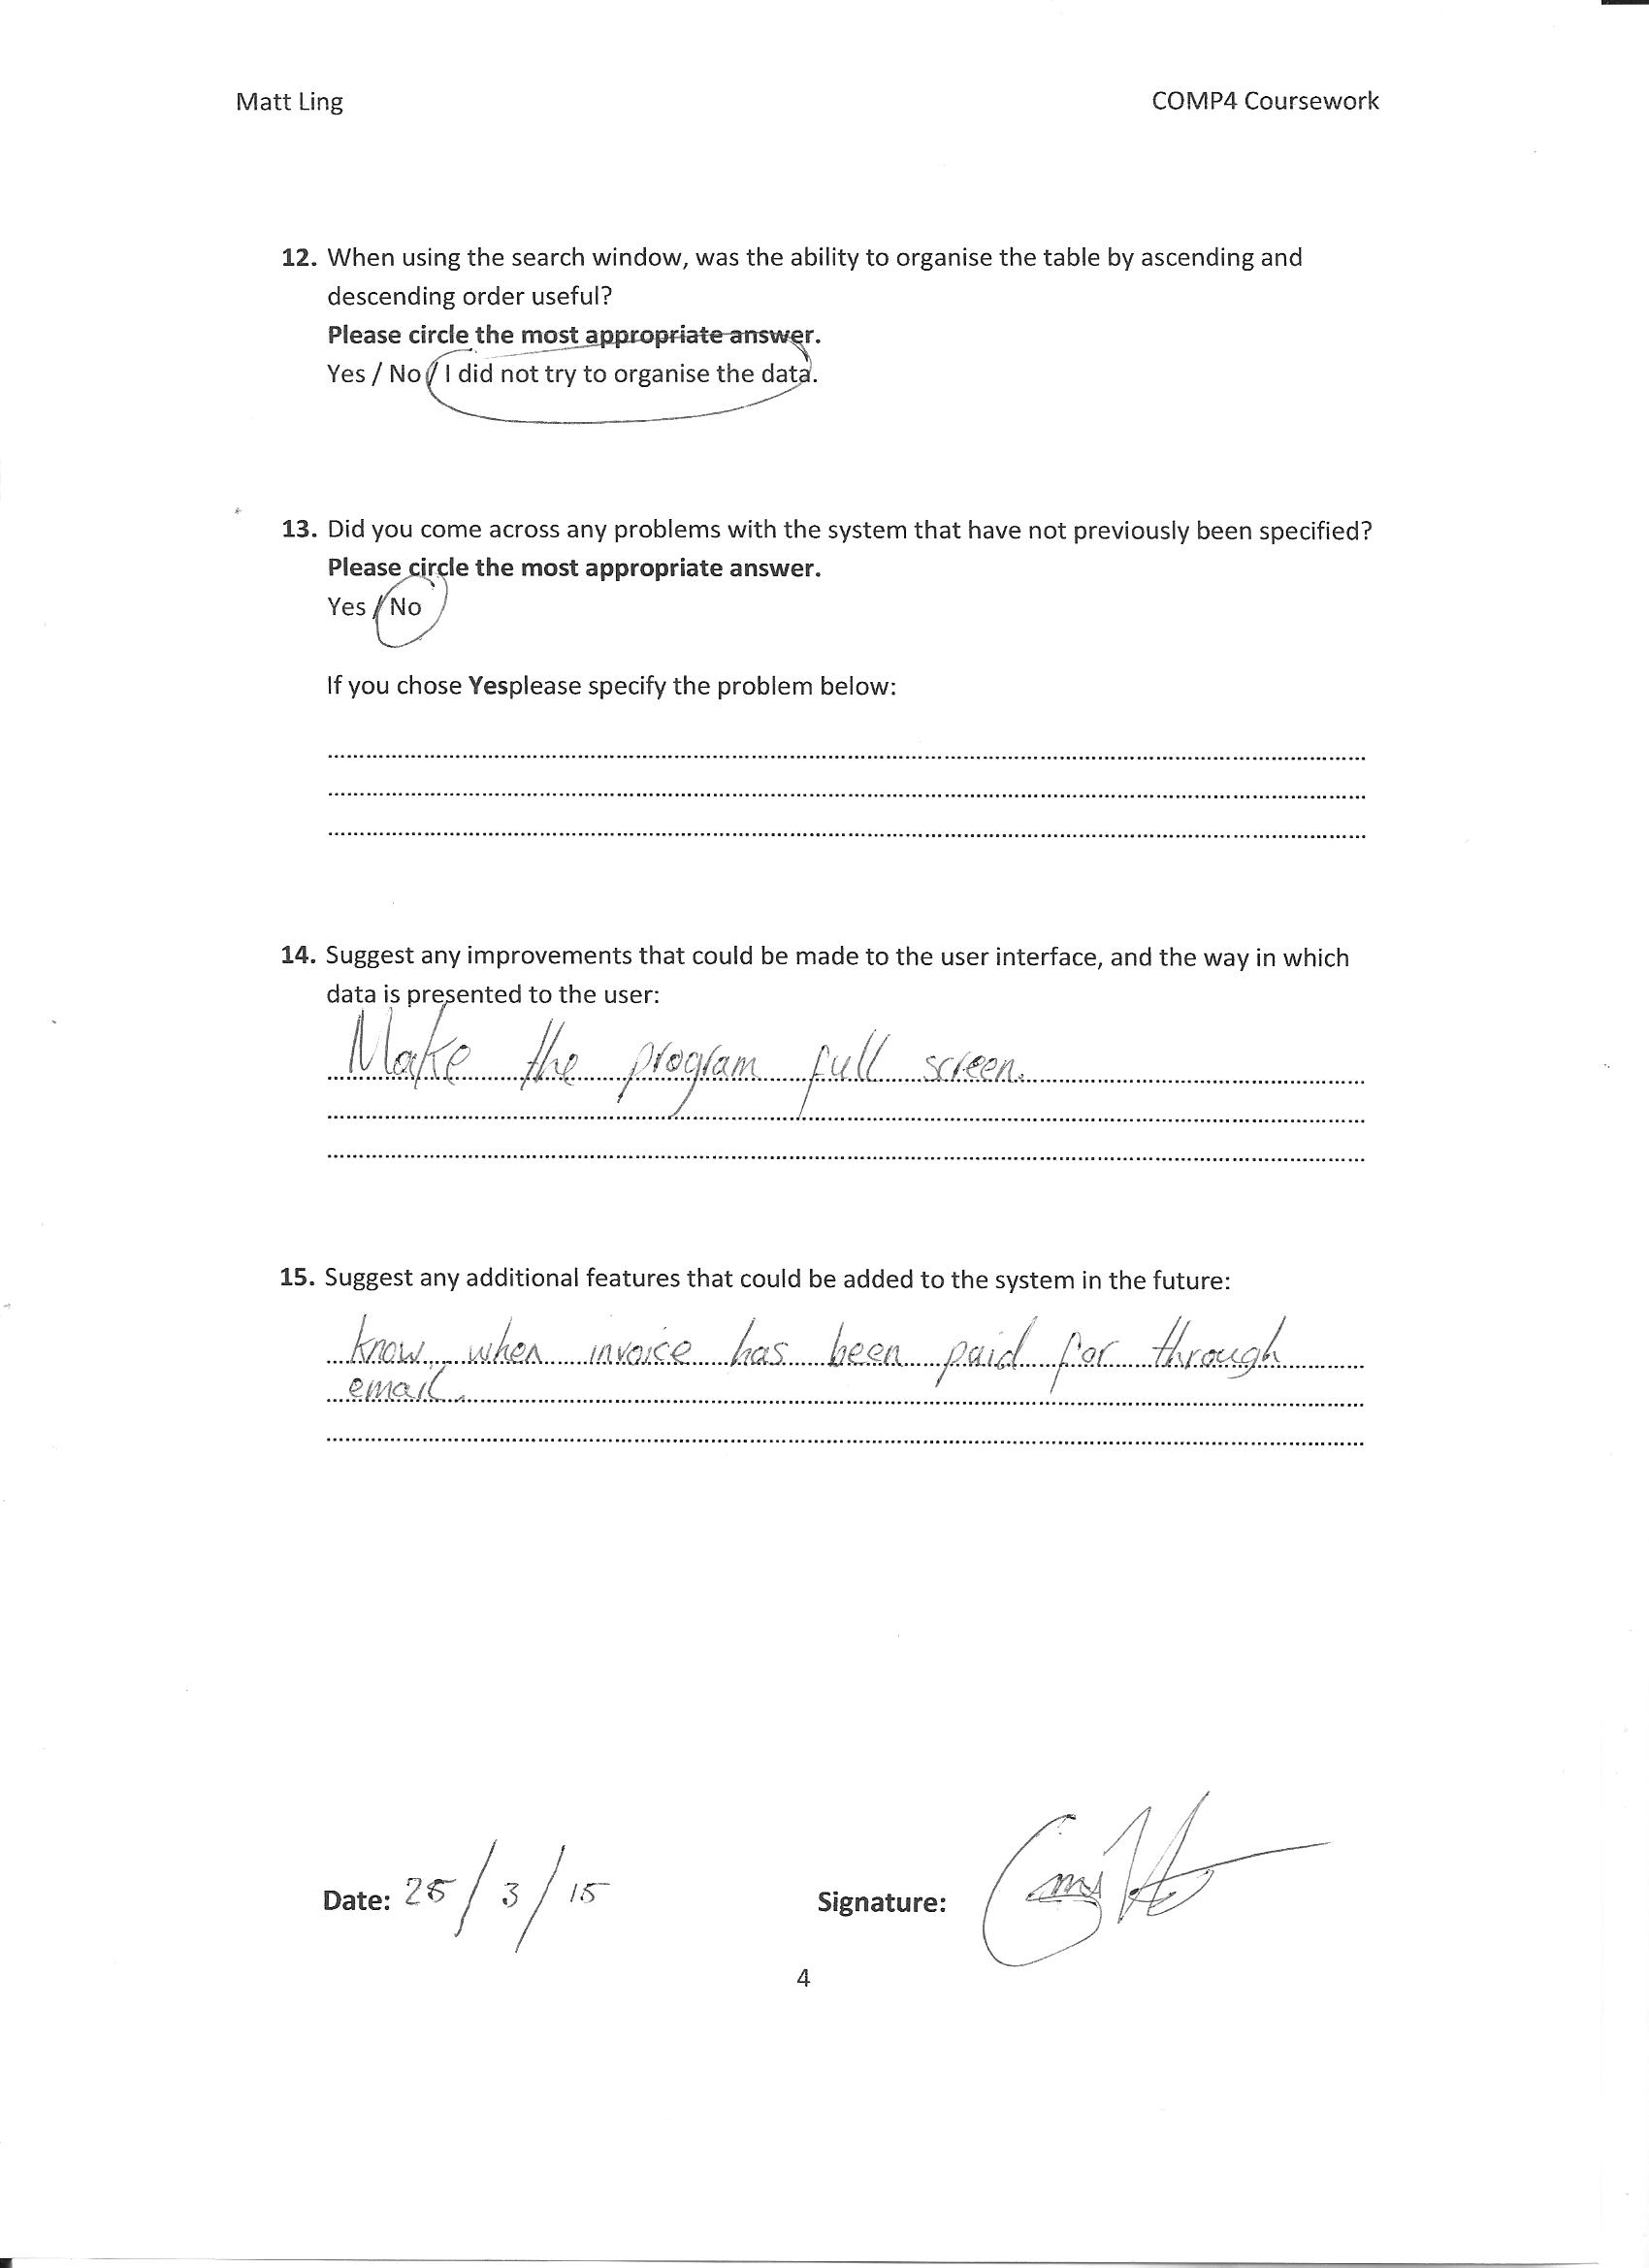
\includepdf{./EvaluationImages/questionaire-5-page-4.jpg}

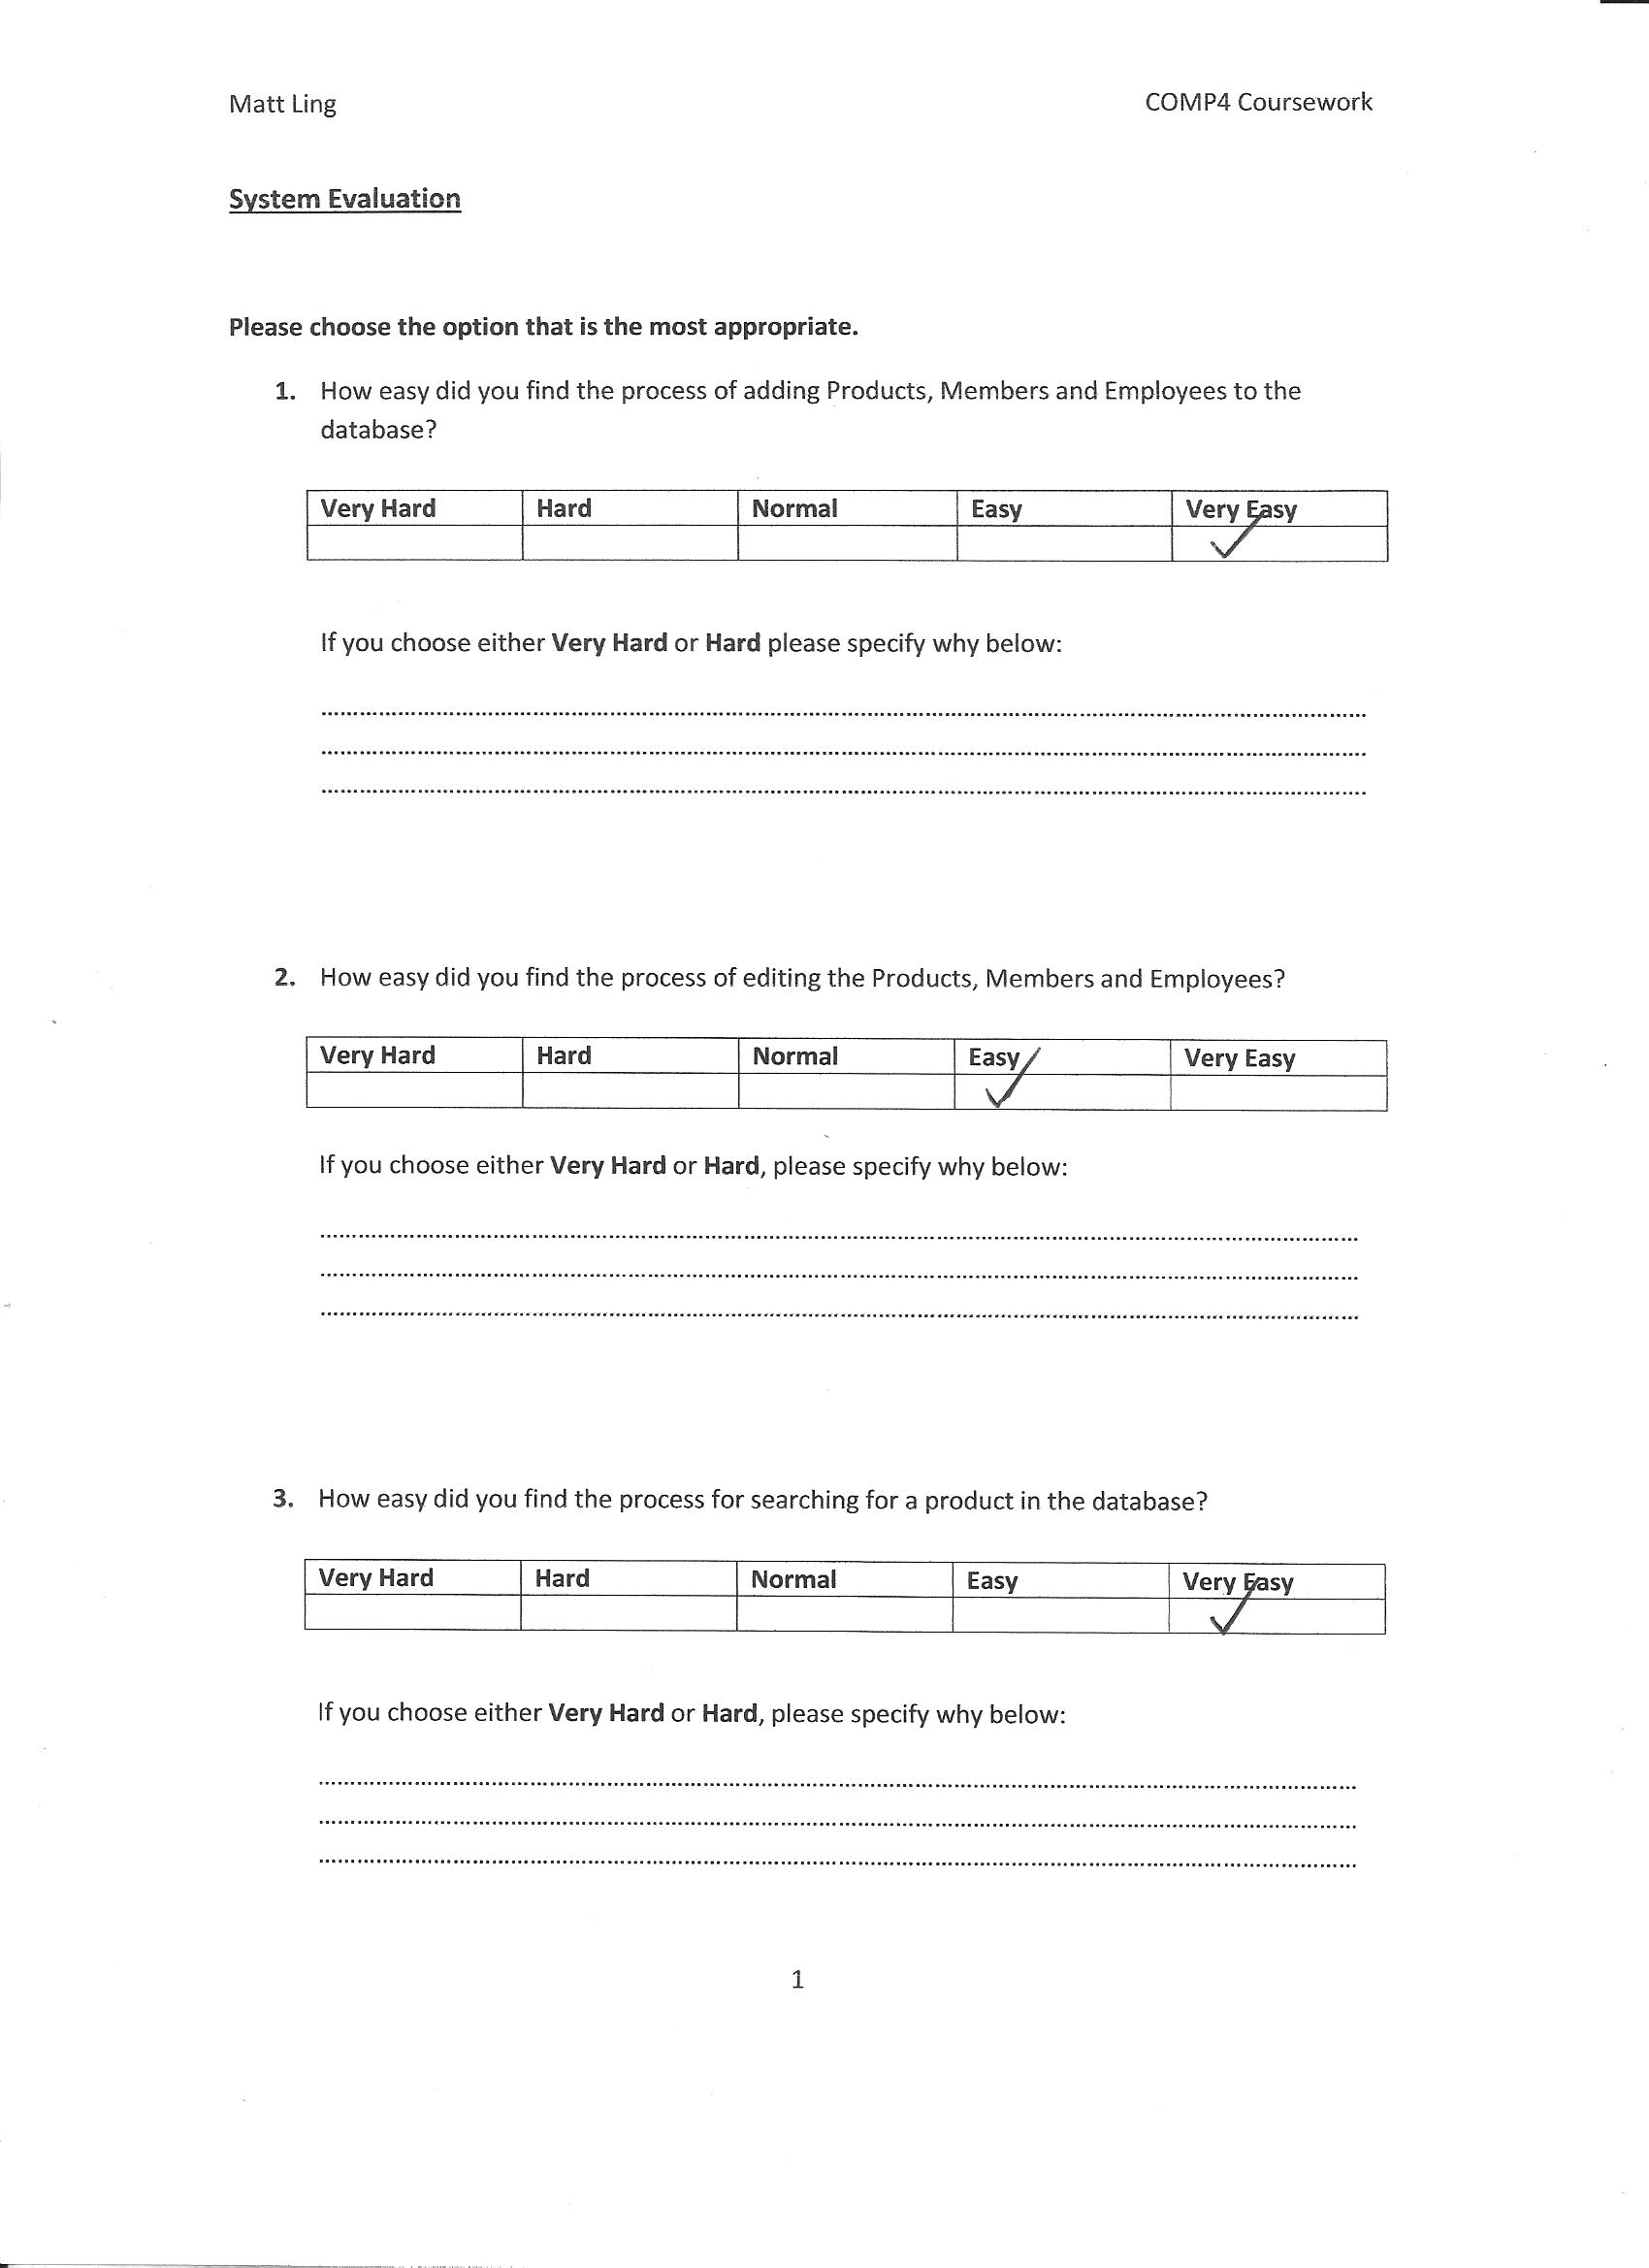
\includepdf{./EvaluationImages/questionaire-6-page-1.jpg}
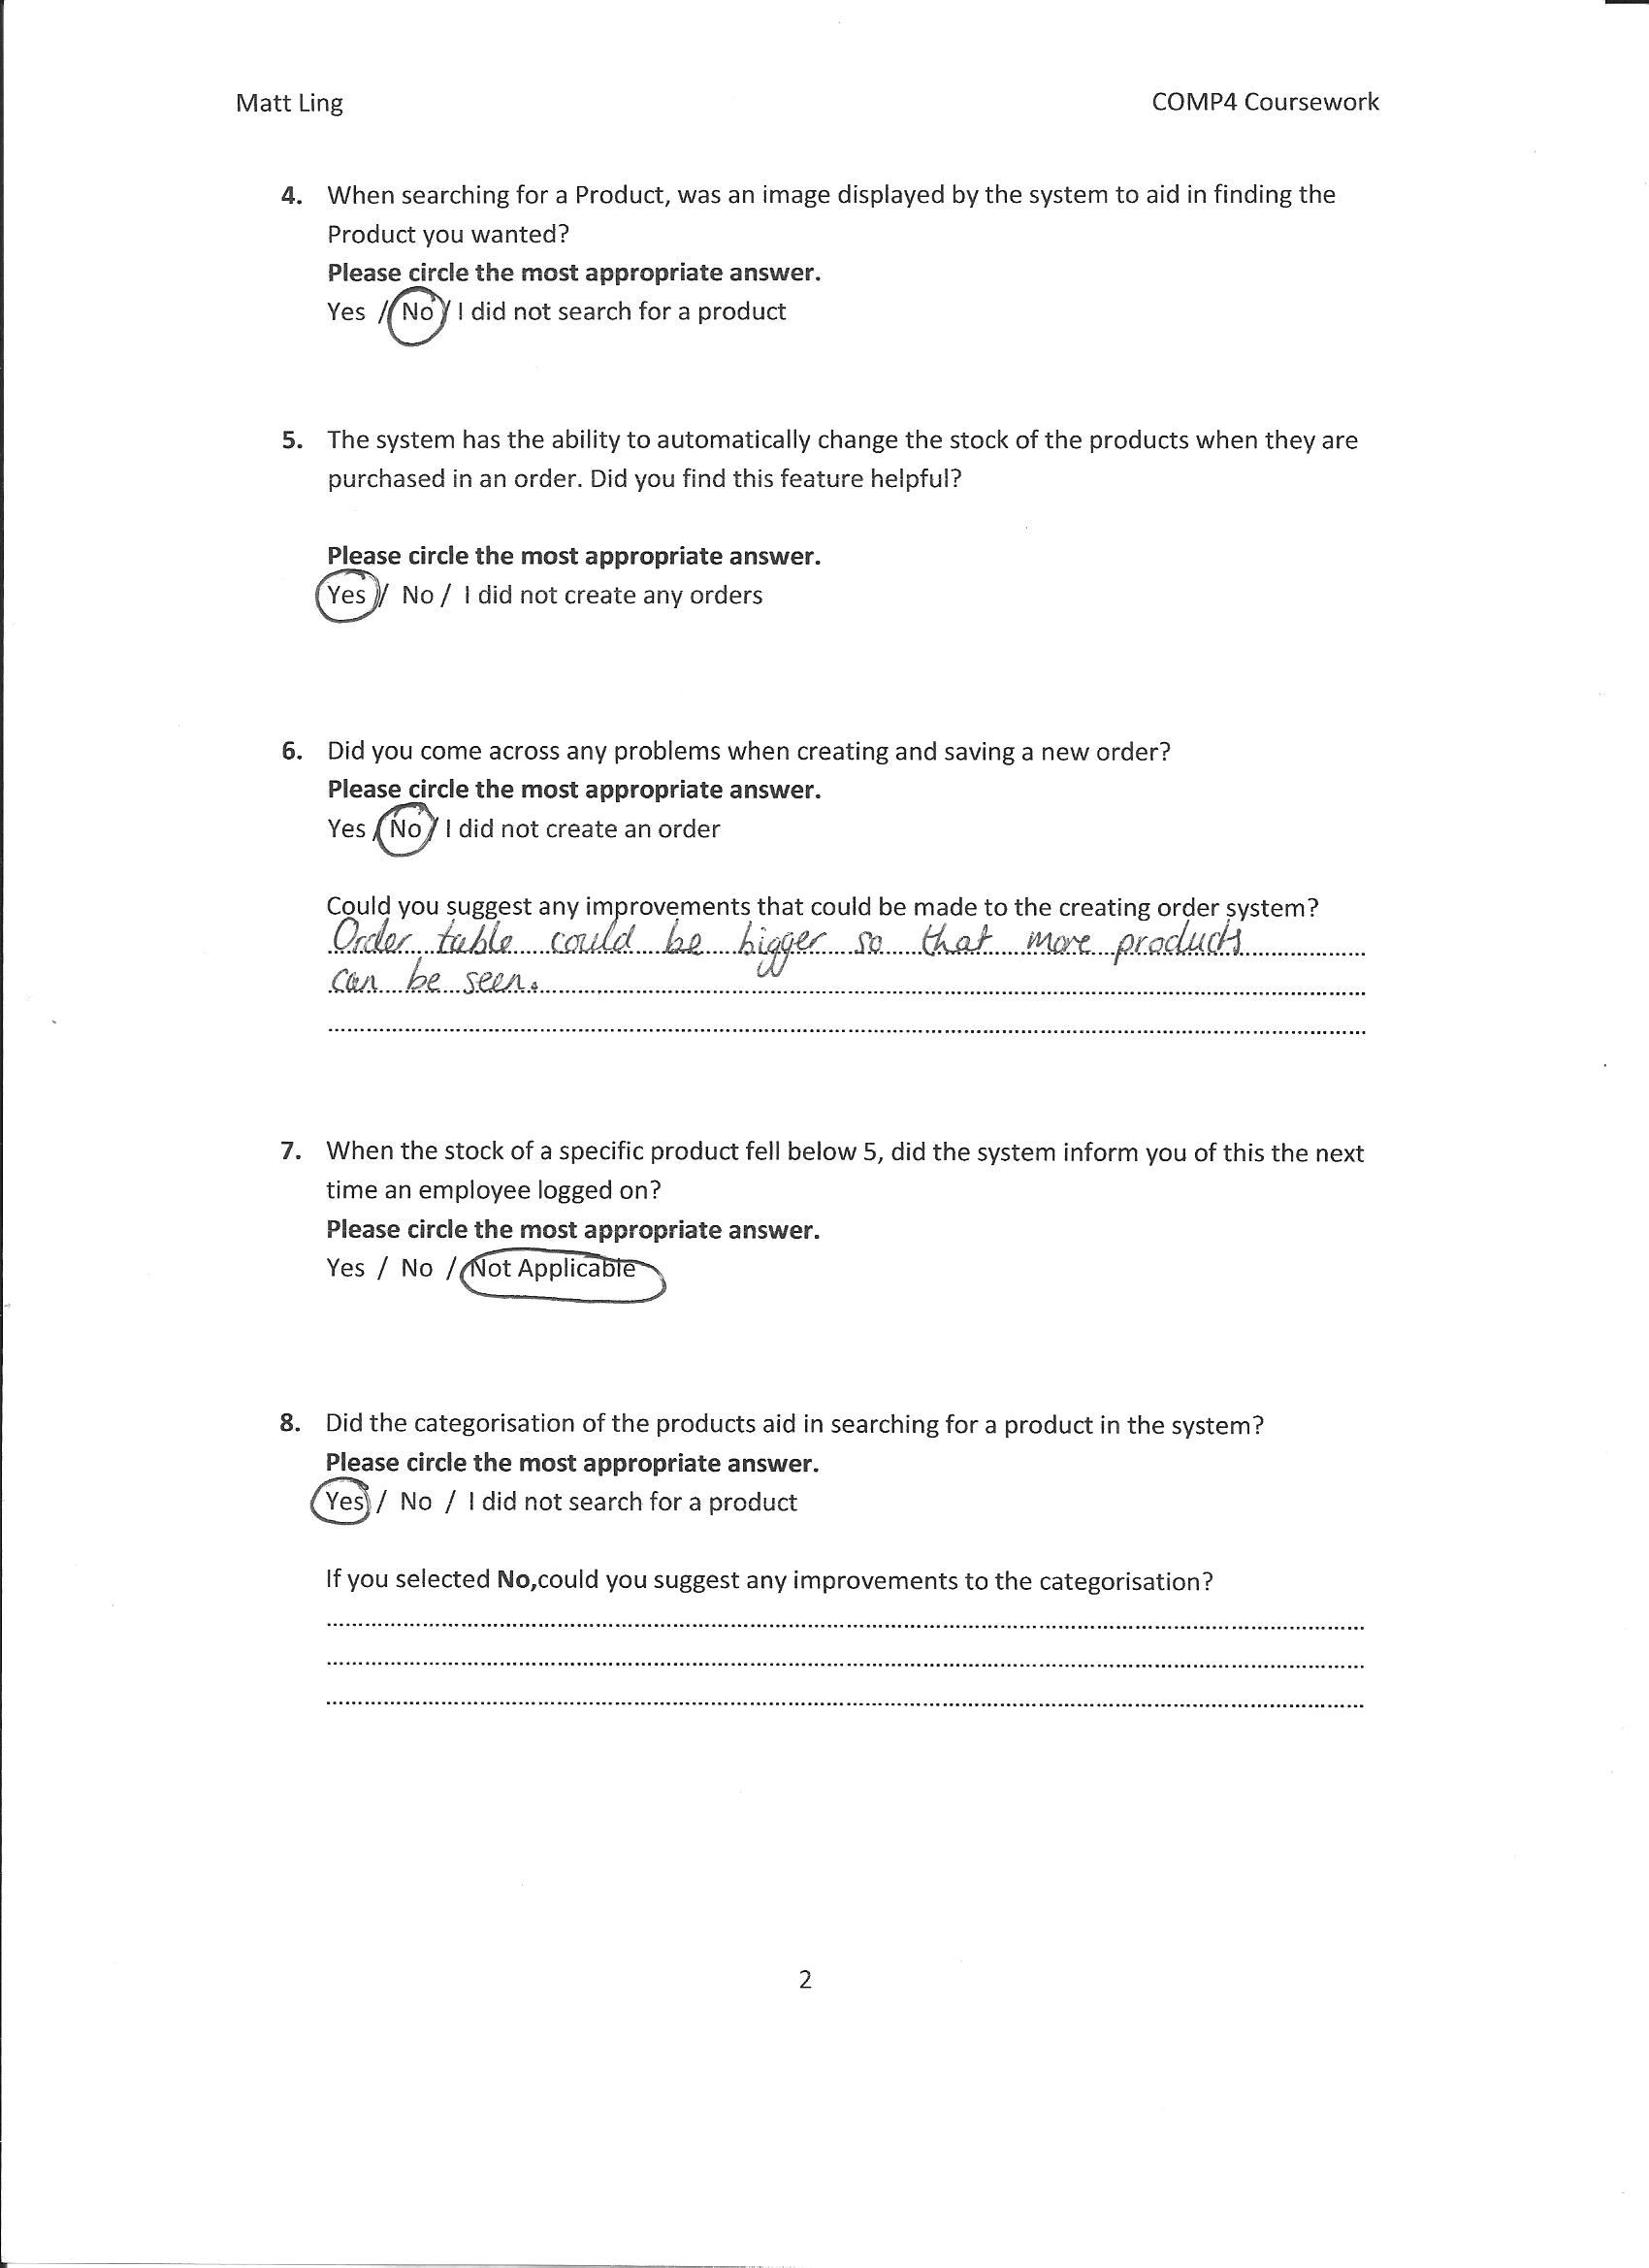
\includepdf{./EvaluationImages/questionaire-6-page-2.jpg}
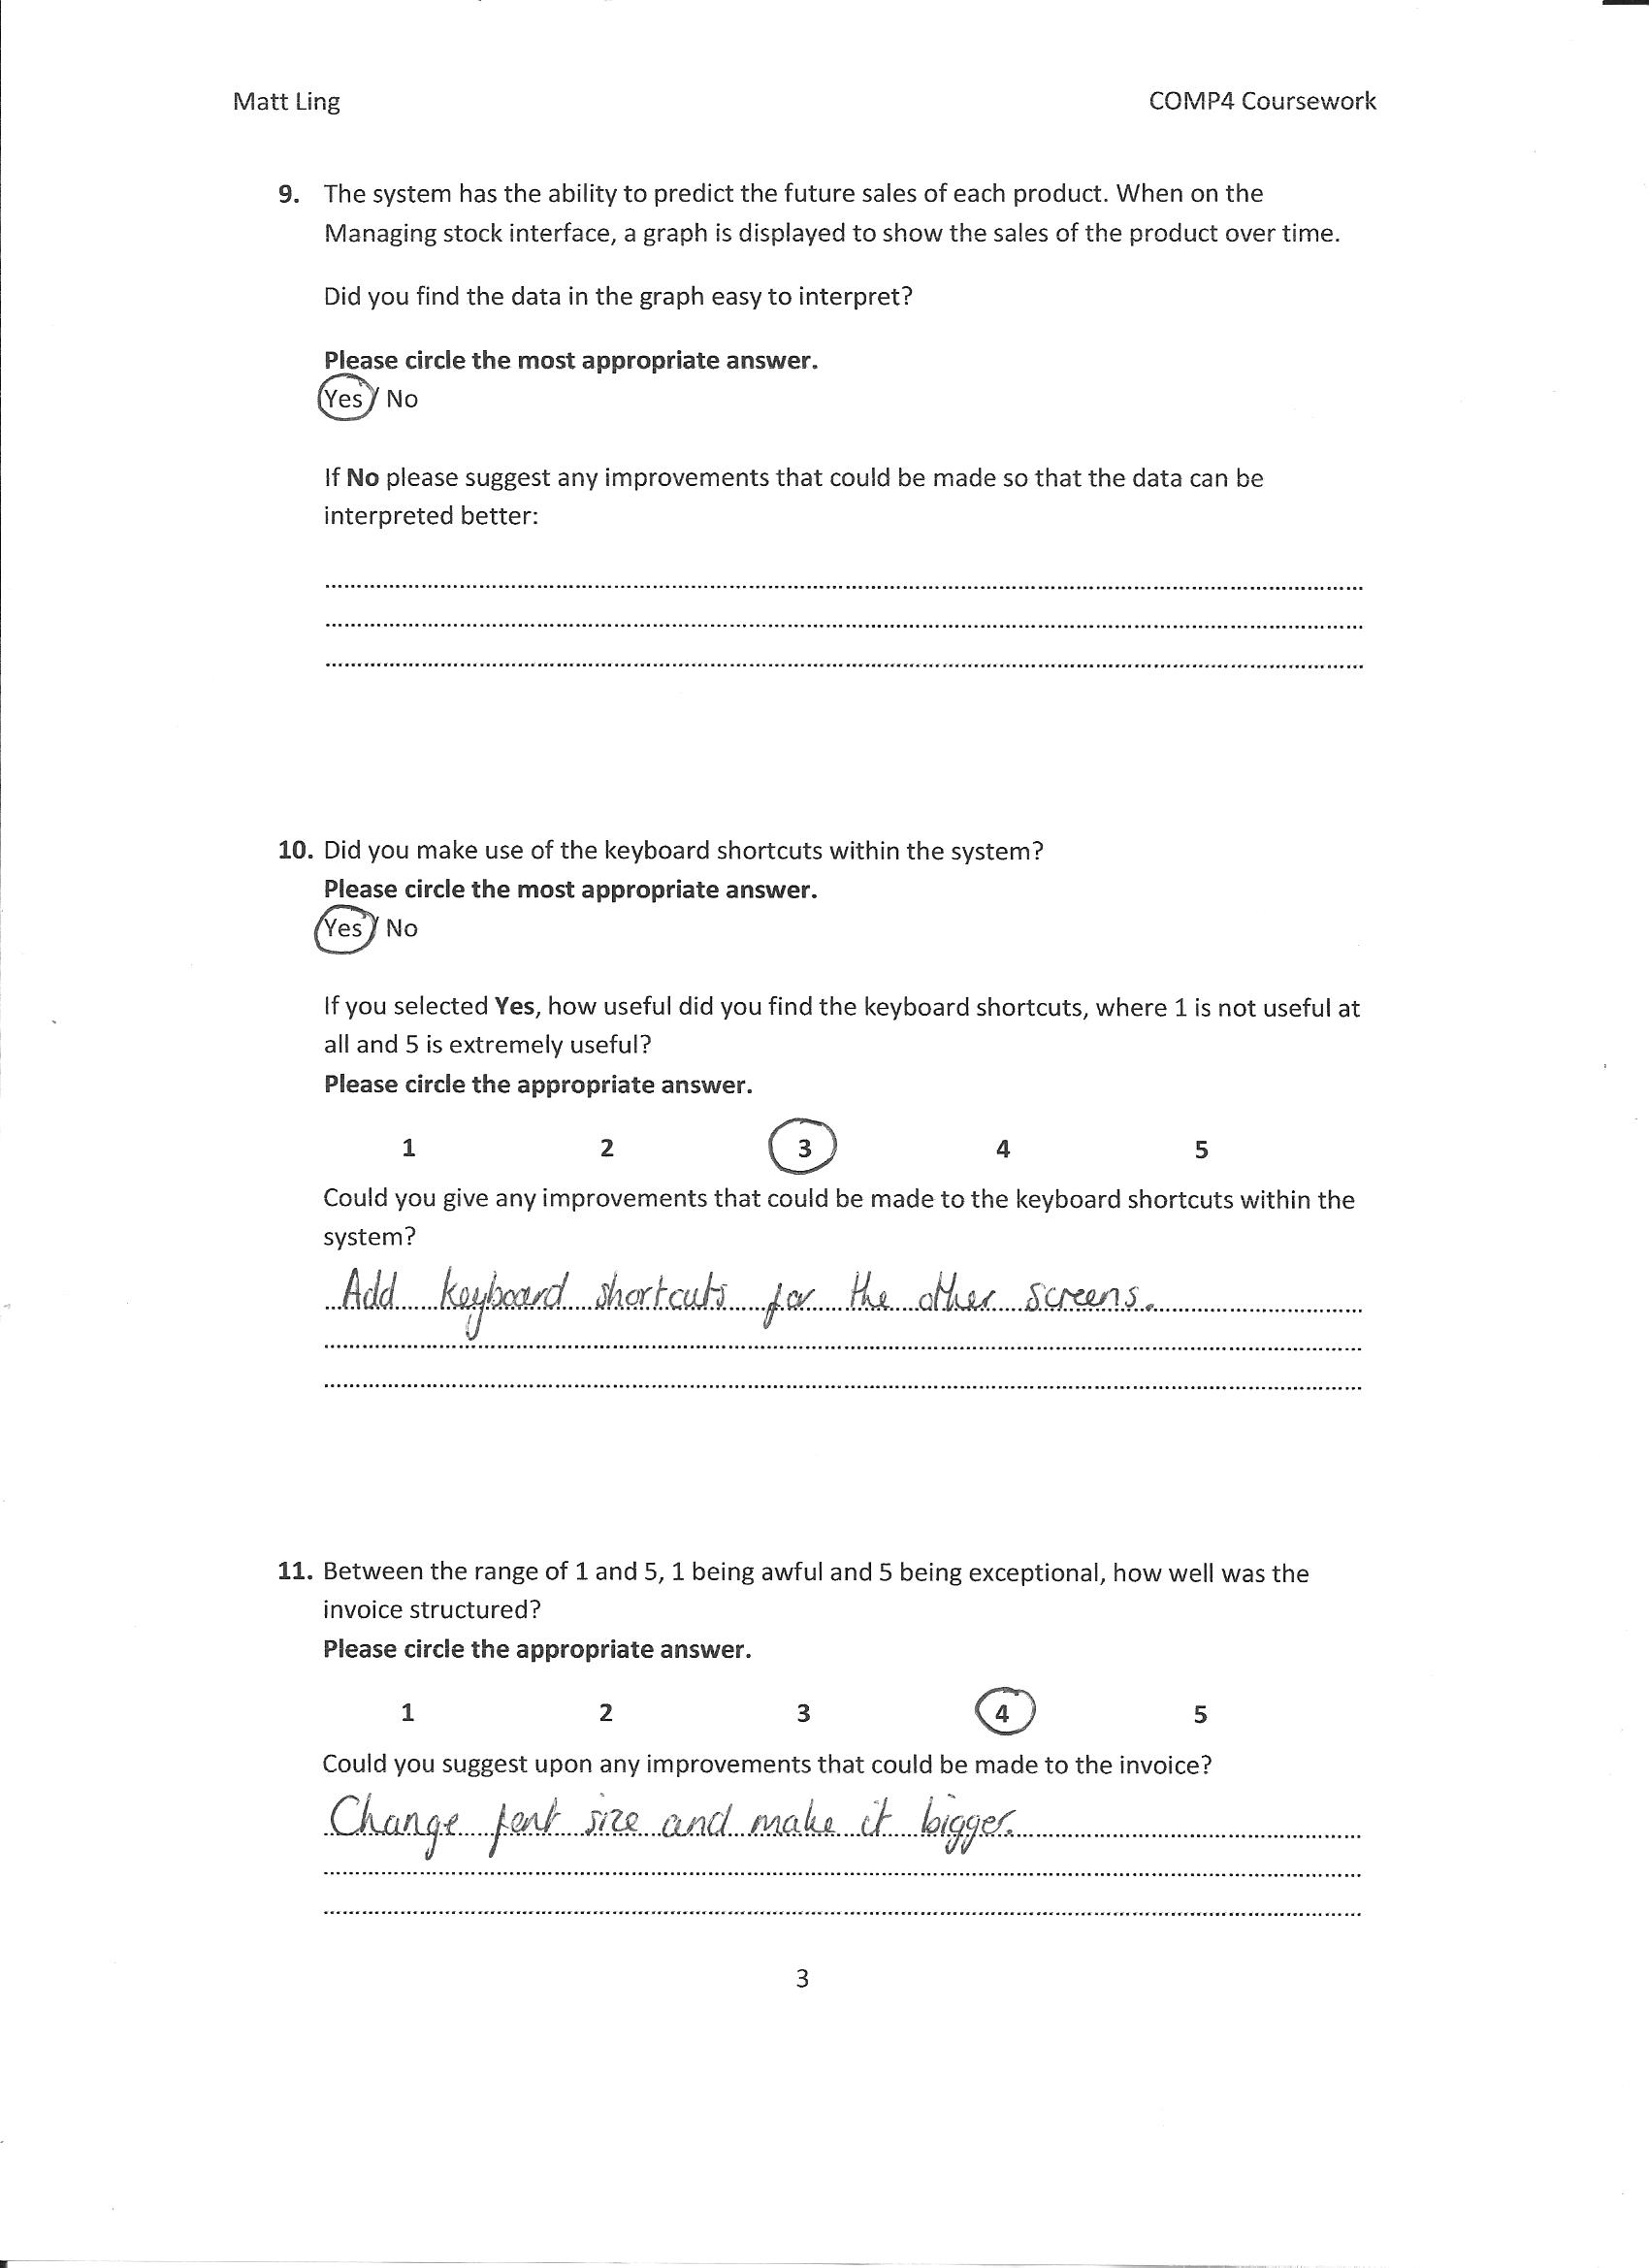
\includepdf{./EvaluationImages/questionaire-6-page-3.jpg}
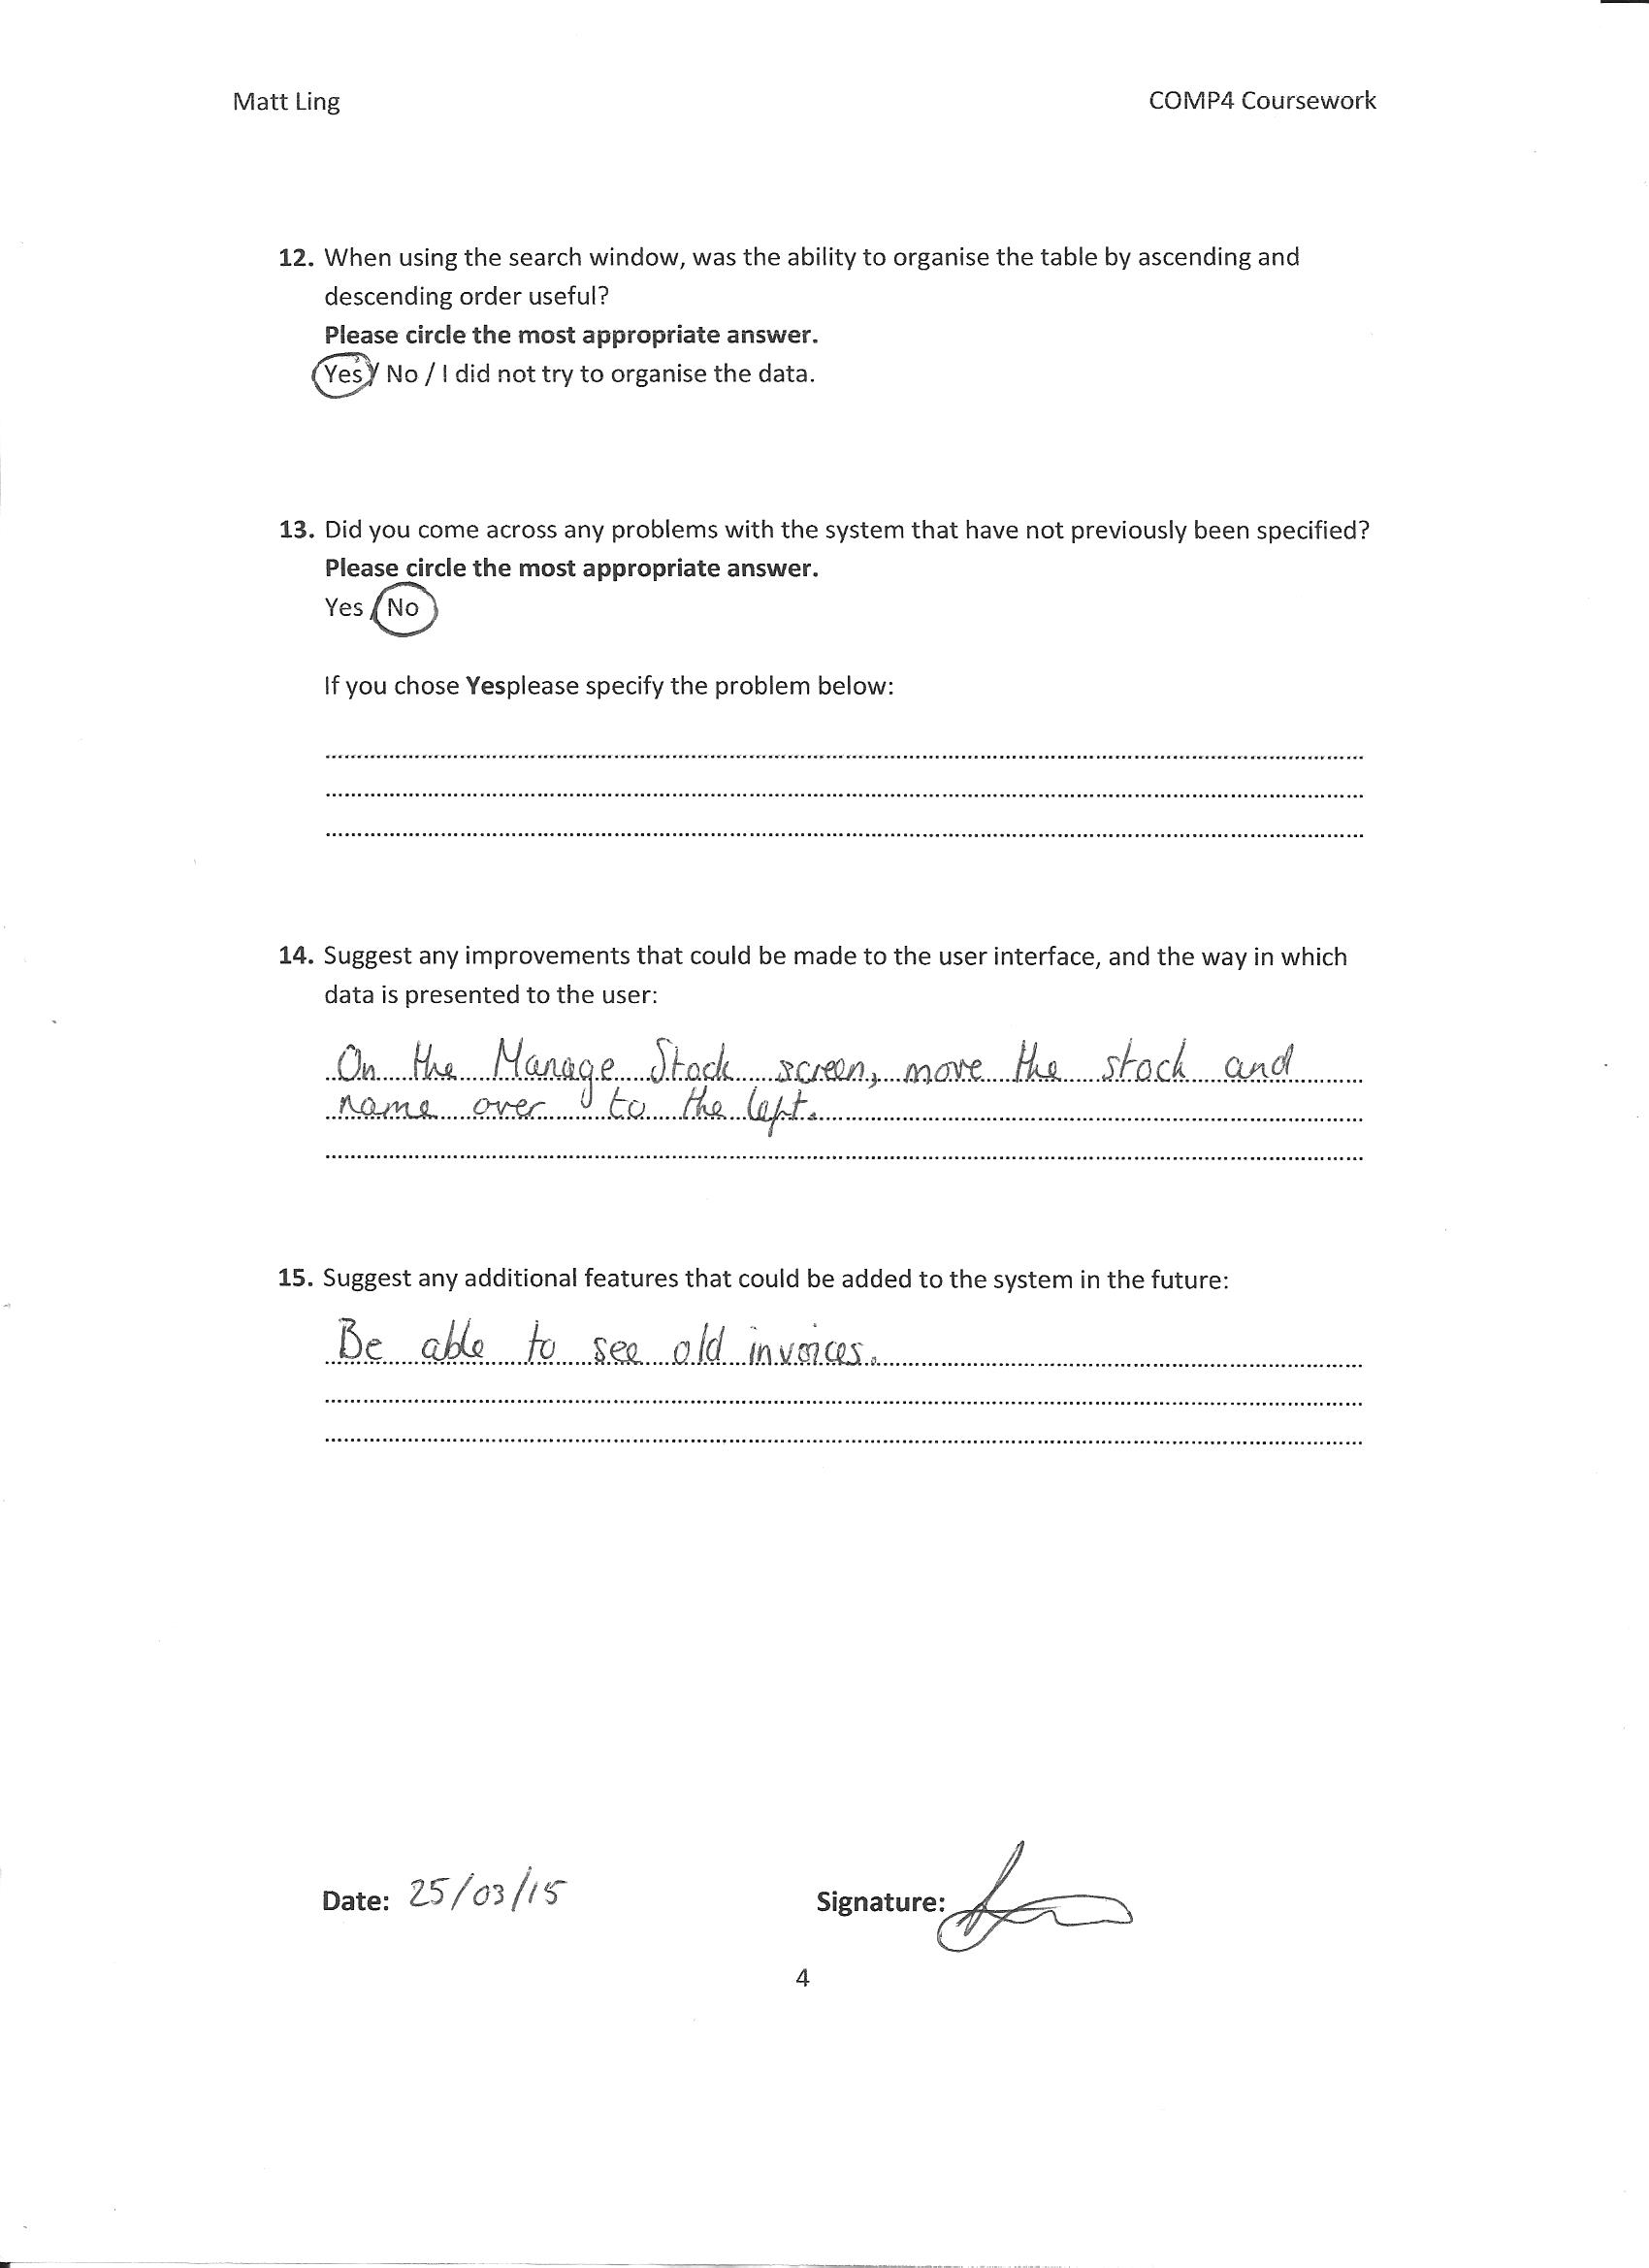
\includepdf{./EvaluationImages/questionaire-6-page-4.jpg}

\subsection{Graphs}

\subsection{Written Statements}
